\documentclass[12pt, oneside]{book}

%Typography and language
\usepackage[utf8]{inputenc}
\usepackage[italian]{babel}
\renewcommand{\familydefault}{\sfdefault}

%Layout
\usepackage[top=1in, bottom=1.25in, left=1.25in, right=1.25in]{geometry}

%Graphics
\usepackage{graphicx}

\usepackage{tabularx}
\usepackage{array}
\usepackage[dvipsnames]{xcolor}
\usepackage{color}
\usepackage{hyperref}
\hypersetup{
    colorlinks,
    linkcolor={blue}, 
    urlcolor={blue}
}

%Math
\usepackage{amsmath}
\usepackage{amssymb}
\usepackage{amsthm}
    \theoremstyle{plain} 
    \newtheorem{thm}{Teorema}[section] 
    \newtheorem{cor}[thm]{Corollario} 
    \newtheorem{lem}[thm]{Lemma} 
    \newtheorem{prop}[thm]{Proposizione} 
    \theoremstyle{definition} 
    \newtheorem{defn}{Definizione}[chapter] 
    \theoremstyle{remark} 
    \newtheorem{oss}{Osservazione} 
\def\ojoin{\setbox0=\hbox{$\bowtie$}%
  \rule[-.02ex]{.25em}{.4pt}\llap{\rule[\ht0]{.25em}{.4pt}}}
\def\leftouterjoin{\mathbin{\ojoin\mkern-5.8mu\bowtie}}
\def\rightouterjoin{\mathbin{\bowtie\mkern-5.8mu\ojoin}}
\def\fullouterjoin{\mathbin{\ojoin\mkern-5.8mu\bowtie\mkern-5.8mu\ojoin}}

%Code
\usepackage{listings}
\lstset{ 
  backgroundcolor=\color{white}, 
  breaklines=true,                 
  captionpos=b,                   
  commentstyle=\color{green},    
  extendedchars=true,  
  mathescape = true,
  frame=single,	                   
  keepspaces=true,                 
  keywordstyle=\color{blue},      
  language=SQL,                 
  morekeywords={*,...},          
  numbers=left,                    
  numbersep=5pt,                   
  numberstyle=\tiny\color{black}, 
  rulecolor=\color{black},        
  showspaces=false,                
  showstringspaces=false,          
  stepnumber=2,                   
  stringstyle=\color{orange},     
  tabsize=2,	                   
  title=\lstname                   
}


\title{Basi di dati}
\author{Elisa Solinas \\
    Corso dei proff. Ruggero Pensa (Teoria)\\
    \large Sara Capecchi (Progettazione)\\
    \large Luca Anselma (SQL)}
\date{A.A. 2016/2017 
    \\Updated on \today}

\begin{document}

\maketitle
\tableofcontents

\part{Teoria}
\chapter{Modello Relazionale}

\section{Relazione}
Una {relazione} è definita da uno {schema} e dalle {istanze} della relazione (dette anche {stato} della relazione)

\section{Attributo}
L'attributo di una relazione (attributo relazionale) è definito come una coppia $A_i:T_i$ dove $T_i$ è il tipo dell'attributo e $A_i$ è il nome dell'attributo.

\subsection{Tipologia}
Un tipo $T_i$ è caratterizzato da:
    \begin{itemize}
        \item{$T_i$: nome \textbf{identitificativo} del tipo}
        \item{$D_i$: \textbf{dominio} di valori}
        \item{Collezione di \textbf{operazioni} abilitate ad agire su $D_i$}
        \item{Operazioni di \textbf{confronto} su $D_i$}
    \end{itemize}
\textbf{Tipi standard}: \texttt{Integer}, \texttt{Real}, \texttt{String}, \texttt{Char}, \texttt{Date}, \texttt{Boolean}\\
\textbf{Tipi utente}: \text{tipo enumerativo}.

\subsection{Dominio}
Un tipo è sempre associato ad un dominio, ovvero a un insieme (potenziale infinito) di valori.\\\\
Possiamo immaginare una funzione
    \begin{equation}\begin{aligned}
        \text{dom}(A_i) = D_i
    \end{aligned}\end{equation}

\subsection{Valore nullo}
Per i casi in cui si riveli necessario inserire delle tuple con attributi mancanti in una relazione, è previsto un \textbf{valore nullo} (\texttt{NULL}), un vero e proprio valore, con la seguente proprietà generale:
    \begin{equation}\begin{aligned}
        \forall T_i, \quad \texttt{NULL} \in D_i
    \end{aligned}\end{equation}
Cioé, il valore \texttt{NULL} appartiene al dominio $D_i$ di qualsiasi tipo $T_i$.

\section{Schema di una relazione}
Lo \textbf{schema di una relazione} è un insieme di attributi, espressi con la seguente notazione:
    \begin{equation}\begin{aligned}
        \{  A_1:T_1, ..., A_n:T_n   \}\\
        R ( A_1:T_1, ..., A_n:T_n   )
    \end{aligned}\end{equation}
Spesso, per semplificare, si sottintende il tipo (che, però, deve sempre essere specificato nei DBMS):
    \begin{equation}\begin{aligned}
        \{  A_1:T_1, ..., A_n:T_n   \}
        \quad \rightarrow \quad
        \{  A_1, ..., A_n   \}\\
        R ( A_1:T_1, ..., A_n:T_n   )
        \quad \rightarrow \quad
        R ( A_1, ..., A_n)
    \end{aligned}\end{equation}  
Definiamo l'insieme di attributi $A$ come:
    \begin{equation}\begin{aligned}
        A: \{  A_1:T_1, ..., A_n:T_n   \}
    \end{aligned}\end{equation}
Possiamo utilizzare la seguente notazione per indicare lo schema $R$:
    \begin{equation}\begin{aligned}
       R(A)
    \end{aligned}\end{equation} 

\section{Grado di una relazione}
La \textbf{cardinalità} $|A|$, anche detta \textbf{grado} della relazione, di uno schema di relazione è data dal numero di attributi dello schema.\\\\
L'insieme di attributi di uno schema di relazione è sempre un insieme non vuoto. Ergo:
    \begin{equation}\begin{aligned}
        |A| \geq 1
    \end{aligned}\end{equation}

\section{Istanza di una relazione}
Dato uno schema:
    \begin{equation}\begin{aligned}
        A: \{   A_1:T_1, ..., A_n:T_n\}
    \end{aligned}\end{equation}
Per semplicità, supponiamo che l'insieme $A$ sia ordinato.\\\\
L'\textbf{istanza}, o \textbf{stato} $r$ di una relazione è definito come un insieme di tuple per cui vale la proprietà:
    \begin{equation}\begin{aligned}
        <v_1, ..., v_n>:\\
        \forall i \quad v_i \in \text{dom}(A_i)
    \end{aligned}\end{equation}

\section{Cardinalità di una relazione}
La \textbf{cardinalità} $|r|$ dell'istanza di una relazione $r$ è data dal numero di tuple appartenenti alla relazione $r$ ed è detta semplicente \textbf{cardinalità della relazione}.\\\\
Contrariamente alla relazione, l'istanza di una relazione può essere vuota:
    \begin{equation}\begin{aligned}
        |r| \geq 0
    \end{aligned}\end{equation}

\section{Notazioni ibride}
Per indicare le relazioni utilizziamo lettere maiuscole:
    \begin{equation}\begin{aligned}
        R \text{ oppure } PAZIENTI
    \end{aligned}\end{equation}
Per indicare l'istanza delle relazioni utilizziamo lettere minuscole:
    \begin{equation}\begin{aligned}
        r \text{ oppure } pazienti
    \end{aligned}\end{equation}
Specifichiamo lo schema anche per le istanze:
    \begin{itemize}
        \item{$r(A_1, ..., A_n)$ o $pazienti(COD, Cognome, Nome, Residenza, AnnoNascita)$}
        \item{$r(R)$ o $pazienti(PAZIENTI)$: poco usate.}
        \item{$r$ o $pazienti$: se lo schema è ben chiaro}
    \end{itemize}
Possiamo usare anche la notazione tabellare:
    \begin{figure}[h!]
        \centering
        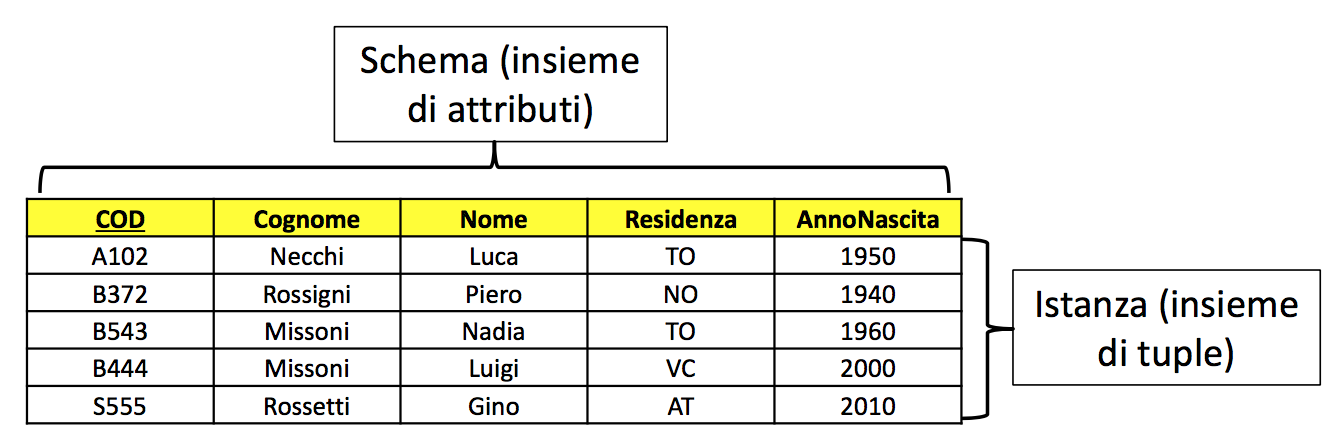
\includegraphics[scale = 0.5]{01/img01}
        \caption{Notazione tabellare}
    \end{figure}
Ciascuna relazione è definita da una coppia:
    \begin{equation}\begin{aligned}
        <R, r>
    \end{aligned}\end{equation}
dove $R$ è lo schema della relazione e $r$ è l'instanza della relazione.

\section{Tupla}
Data la relazione $r(A_1, ..., A_n)$,per indicare una singola \textbf{tupla} si usa la notazione
    \begin{equation}\begin{aligned}
        t = <v_1, ..., v_n>
    \end{aligned}\end{equation}
Poiché $t$ prende valori all'interno della relazione $R$:
    \begin{equation}\begin{aligned}
        t \in r (A_1, ..., A_n)
    \end{aligned}\end{equation}
    
\subsection{Valori di una tupla}
Per indicare il valore di una tupla $t$ in corrispondenza dell'attributo $A_i$ o di un insieme di attributi $A_i, ..., A_k$ si utilizzano le seguenti notazioni:
    \begin{equation}\begin{aligned}
        t[A_i] = v_i\\
        t.A_i = v_i\\
        t[A_i, ..., A_k] = <v_i, ..., v_k>\\
        t.(A_i, ..., A_k) = <v_i, ..., v_k>
    \end{aligned}\end{equation}
Per richiamare la tupla su tutti gli attributi si utilizzano le seguenti notazioni:
    \begin{equation}\begin{aligned}
        t, t[A], t.A
    \end{aligned}\end{equation}
Non essendo importante l'ordine degli attributi, la tupla non è altro che una \textbf{rappresentazione tabellare} che fa corrispondere a ogni attributo un valore del suo dominio:
    \begin{equation}\begin{aligned}
        t: A \rightarrow D
    \end{aligned}\end{equation}
    
\subsubsection{Esempio}
    \begin{center}\begin{tabular}{|c|c|} \hline
        \textbf{A} & \textbf{D}\\ \hline
        COD & A102 \\ \hline
        Cognome & Necchi \\ \hline
        Nome & Luca \\ \hline
        Residenza & TO \\ \hline
        AnnoNascita & 1950 \\ \hline
    \end{tabular}\end{center}
Possiamo adesso definire l'istanza $r$ di una relazione è dunque un insieme di funzioni
    \begin{equation}\begin{aligned}
        \{  t_1, ..., t_n   \}
    \end{aligned}\end{equation}
Ciascuna funzione $t_i$ definisce una particolare corrispondenza tra attributi e valori.\\
Le funzioni $t_i$ sono tutte distinte tra loro: ciò significa che in una relazione non può esistere una tupla identica a un'altra.\\\\
La tupla $t$ è \textbf{compatibile} con lo schema $A$ di una relazione se:
    \begin{itemize}
        \item{$t$ è una \textbf{funzione totale} su $A$.}
        \item{Ogni valore prodotto da $t$ appartiene a $D$.}
        \item{Vale il vincolo:
            \begin{equation}\begin{aligned}
                \forall A_i, \quad t.A_i \in \text{dom}(A_i)
            \end{aligned}\end{equation}}
    \end{itemize}

\section{Vincoli locali}
I \textbf{vincoli locali} sono caratterizzazioni dei valori possibili delle tuple in modo che tali valori rispettino (non siano in contrasto con) la realtà che vogliamo rappresentare.

\subsection{Vincolo locale di dominio}
Per ogni attributo abbiamo un insieme ben definito (anche infinito) di valori possibili.\\
Inoltre:
\begin{itemize}
    \item{Qualsiasi valore $v$ del dominio $D_i$ è atomico}
    \item{Un attributo il cui valore è una relazione non è atomico (solo alcuni DBMS, tra cui Oracle, lo permettono).}
\end{itemize}
Una relazione è \textbf{in prima forma normale} quando tutti gli attributi sono abbinati a domini di \textbf{valori atomici}.

\subsection{Vincolo sui valori nulli}
Un vincolo \texttt{NOT NULL} su un attributo $A_i$ è soddisfatto se, per ogni $t \in r$, il valore $t.A_i$ non è nullo.\\
Il funzionamento \textbf{pratico} è il seguente: al momento del caricamento dei dati in una tabella, il DBMS verifica che la tupla sia compatibile e che i valori degli attributi per cui è attivo il vincolo \texttt{NOT NULL} siano non nulli.

\subsection{Altri vincoli}
I DBMS forniscono la sintassi necessaria per la verifica dei seguenti vincoli:
    \begin{itemize}
        \item{\textbf{Restrizioni sui domini}: specificano i valori che non possono essere assunti da un particolare attributo.\\
            \textbf{ES:} una persona non può avere più di 120 anni, e non può essere nata nel futuro.\\
            \textbf{ES:} la temperatura corporea di un paziente non può superare i 42 gradi ed essere inferiore ai 34.}
        \item{\textbf{Confronti sui domini}: esprimono legami che devono essere rispettati da due o più attributi.\\
            \textbf{ES:} la data d'inizio ricovero dev'essere antecedente alla data di fine ricovero.}
    \end{itemize}

\subsection{Vincolo di identificazione}
Il vincolo di identificazione ci permette di identificare univocamente una tupla all'interno di uno schema, ed è espresso attraverso il vincolo di \textbf{chiave relazionale}.\\\\
Le chiavi relazionali possono essere composte da più valori, come nella tabella $RICOVERI$.\\\\
La nozione di vincolo di chiave relazionale è solitamente definita dal contesto applicativo (es. $COD$ dei $pazienti$ o $MATR$ dei medici).\\\\
Nella relazione di Codd gli elementi (tuple) dell'insieme (istnza) $r$ devono essere tutti distanti tra di loro.

\subsection{Definizione di superchiave}
Per poter definire in maniera formale il vincolo di chiave relazionale dobbiamo introdurre prima la nozione di superchiave.\\\\
Data una relazione $r(A)$, un sottoinsieme di attributi $sk \subseteq A$ è una \textbf{superchiave} 
    \begin{equation}\begin{aligned}
        \forall i,j \quad 
        (t_i[sk] = t_j[sk]) \rightarrow (t_i[A] = t_j[A])
    \end{aligned}\end{equation}
\textbf{ES:} nella tabella $PAZIENTI$, $(COD, Nome)$ è una superchiave.

\subsection{Chiave candidata}
$k \subseteq A$ è \textbf{chiave candidata} se:
    \begin{itemize}
        \item{$k$ è superchiave di $R$}
        \item{$k$ è superchiave \textbf{minimale} di $R$ (ogni sottoinsieme proprio di $k$ non deve soddisfare le condizione di superchiave).}
    \end{itemize}    
\textbf{ES:} $COD$ è superchiave, quindi $\{COD; Cognome\}$ non è chiave candidata.\\\\
Se $sk$ è una superchiave, allora $sk \subseteq w \subseteq A$ è una superchiave, quindi sono valide le seguenti \textbf{proprietà}:
    \begin{itemize}
        \item{$A$ è necessariamente una superchiave (per la definizione stessa di istanza, ogni tupla è distinta).}
        \item{$A$ è superchiave, quindi $A$ deve contenere sempre almneo una chiave candidata.}
    \end{itemize}

\subsection{Chiave principale}
La chiave principale $pk \subseteq A$ è una chiave scelta dal progettista tra tutte le possibili chiavi candidate.\\\\
Tutti gli attributi di una chiave principale devono rispettare in vincolo \texttt{NOT NULL}: una chiave candidata, invece, può ammettere valori nulli.

\section{Correttezza di una relazione}
Un'istanza di relazione $r(A)$ è corretta se ogni tupla $t \in r$ è compatibile con lo schema $A$ e sono soddisfatti tutti i vincoli locali (o intrarelazionali).

\section{Schema di una base dati}
Lo schema di una base dati è un insieme di schemi di relazione tutti con nome:
    \begin{equation}\begin{aligned}
        S = \{  R_1, ..., R_n   \}
    \end{aligned}\end{equation}
$S$ rispetta le seguenti proprietà:
    \begin{itemize}
        \item{I nomi devono essere tutti distinti}
        \item{Ad ogni schema si abbinano i rispettivi vincoli locali}
        \item{Ogni relazione $R_i$ esibisce una chiave principale}
    \end{itemize}

\section{Vincoli globali}
Così come è possibile definire dei vincoli locali (\textbf{intrarelazionali}) su ogni relazione $R$ è altresì possibile definire vincoli globali (\textbf{interrelazionali}) su uno schema di basi di dati $S$.

\subsection{Vincolo di integrità referenziale}
Consideriamo una relazione $R_h(\underline{PK}, ...)$ dove $PK$ è l'insieme di attributi della chiave principale, e una relazione $R_s(..., B, ...)$ dove $B$ è un insieme di attributi qualsiasi.\\\\
Esiste un \textbf{vincolo di integrità referenziale} degli attributi $B$ rispetto alla tavola $R_h$ se:
    \begin{equation}\begin{aligned}
        \forall t_i \\
        (t_i \in r (R_s))
        \quad \rightarrow \quad
        \exists t_j: [(t_j \in r(R_h)) \wedge (t_i[B] = t_j[PK])]
    \end{aligned}\end{equation}
Per poter creare il vincolo è necessario che i domini degli attributi in $PK$ siano compatibili con i domini degli attributi in $B$.    

\subsection{Vincoli globali generali}
I vincoli globali generali sono suggeriti dalle regole imposte dal sistema informativo e sono detti \textbf{regole di business}.\\\\
\textbf{ES:} in un sistema bancario con relazione $CONTOCORRENTE$ e relazione $MUTUO$, tutti i titolari di mutuo devono essere ten

\section{Base dati}
\subsection{Definizione di schema di una base dati}
La definizione dello schema $S$ di una base dati è completata dai vincoli globali.
\subsection{Stato di una base di dati}
Dato uno schema di base dati $S = \{    R_1, ..., R_n   \}$, lo \textbf{stato della base di dati} è definito come:
    \begin{equation}\begin{aligned}
        DB = \{ <R_1,r_1>,  ..., <R_n, r_n>   \}
    \end{aligned}\end{equation}
Dove ogni $r_i$ deve essere corretta e devono essere soddisfatti tutti i vincoli globali.

\section{Considerazione finale sul modello relazionale}
Il modello relazionale è un modello \textbf{orientato ai valori}.\\\\
Quando costruisco informazioni che coinvolgono tuple di relazioni diverse non posso che lavorare sui valori contenuti nelle tuple.\\
L'identificazione (chiave) di una relazione è basata sui valori presenti nella chiave.\\\\
In altri modelli (gerarchico, reticolare) le corrispondenze tra dati avvengono attraverso riferimenti (puntatori).

\chapter{Algebra relazionale}

Il modello relazionale descrive il modello del \textbf{DDL} (Data Definition Language), mentre l'algebra relazionale si occupa del \textbf{DML} (Data Manipulation Language), che manipola le tuple presenti nella base dati.\\\\
Il cuore del DML è il linguaggio di interrogazione.\\
Secondo il modello dell'interrogazione di Codd, ciascuna interrogazione ha come input la base dati e come output una relazione.\\\\
\textbf{ES:} elencare i pazienti ricoverati nel reparto il cui primario è il Dott. Neri; visualizzare cognome, nome e nome del reparto.\\\\
Codd formalizza l'interrogazione utilizzando il paradigma algebrico, cioè una costruzione \textbf{procedurale} dell'interrogazione: ciascuna interrogazione elenca i passi per eseguire l'operazione.\\
La presentazione è però più astratta, in quanto utilizza degli operatori algebrici.\\
Gli operatori dell'algebra relazionale ricevono, come argomenti, relazioni e producono in uscita altre relazioni (dette anche \textbf{relazioni virtuali}).

\section{Operatore selezione}
Data una relazione $r$ su uno schema $A$, l'operatore di selezione viene indicato con
    \begin{equation}\begin{aligned}
        \sigma_{p}(r(A))
    \end{aligned}\end{equation}
Dove $p$ è un predicato e $r(A)$ è l'argomento dell'operatore.\\
La selezione produce una relazione senza nome che ha l'identico schema $A$ della relazione argomento, ma solo le tuple che soddisfano il predicato $p$.

\subsection{Sintassi del predicato di selezione}
Il predicato $p$ è un'espressione booleana di predicati atomici, che possono essere solo di due tipi: confronto tra due attributi, oppure confronto tra un attributo e una costante.

\subsection{Cardinalità della selezione}
La cardinalità della relazione virtuale prodotta dall'operazione di selezione $\sigma_p(r(A))$ è 
    \begin{equation}\begin{aligned}
        0 \leq |\sigma_{p}(r(A))| \leq |r(A)|
    \end{aligned}\end{equation}

\subsubsection{Esempi}
\textbf{ES1:} selezione dei pazienti con residenza a Torino
    \begin{equation}\begin{aligned}
        \sigma_{Residenza = 'TO'}(pazienti)
    \end{aligned}\end{equation}
    \begin{center}\begin{tabular}{|c|c|c|c|c|} \hline
        \textbf{COD} & \textbf{Cognome} & \textbf{Nome} 
        & \textbf{Residenza} & \textbf{AnnoNascita}\\
        \hline
        A102 & Necchi & Luca & TO & 1950\\
        \hline
        B543 & Missoni & Nadia & TO & 1950\\
        \hline
    \end{tabular}\end{center}
\textbf{ES2:} selezione dei pazienti residenti a Torino o a Vercelli
    \begin{equation}\begin{aligned}
        \sigma_{Residenza = 'TO' \wedge Residenza = 'VC'}(pazienti)
    \end{aligned}\end{equation}
    \begin{center}\begin{tabular}{|c|c|c|c|c|} \hline
        \textbf{COD} & \textbf{Cognome} & \textbf{Nome} 
        & \textbf{Residenza} & \textbf{AnnoNascita}\\ \hline
        A102 & Necchi & Luca & TO & 1950\\ \hline
        B543 & Missoni & Nadia & TO & 1950\\ \hline
        B444 & Missoni & Luigi & VC & 2000\\ \hline
    \end{tabular}\end{center}
\textbf{ES3:} selezione dei pazienti non residenti a Torino
    \begin{equation}\begin{aligned}
        \sigma_{\neg Residenza = 'TO'}(pazienti)
    \end{aligned}\end{equation}
    \begin{center}\begin{tabular}{|c|c|c|c|c|} \hline
        \textbf{COD} & \textbf{Cognome} & \textbf{Nome} 
        & \textbf{Residenza} & \textbf{AnnoNascita}\\ \hline
        B372 & Rossigni & Piero & NO & 1940\\ \hline
        B444 & Missoni & Luigi & VC & 2000\\ \hline
        S555 & Rossetti & Gino & AT & 2010\\ \hline
     \end{tabular}\end{center}
     
\section{Operatore proiezione}
Data una relazione $r(A)$ e un insieme di attributi $A_i, ..., A_k$ tutti appartenenti ad $A$, l'operatore di proiezione
    \begin{equation}\begin{aligned}
        \Pi_{A_i, ..., A_k}(r(A))
    \end{aligned}\end{equation}
produce come risultato una relazione avente:
    \begin{itemize}
        \item{Schema: $\{   A_i, ..., A_k   \}$}
        \item{Istanza: tutte le tuple della relazione argomento, ma solo rispetto ai campi $A_i, ..., A_k$}
    \end{itemize}

\subsection{Cardinalità della proiezione}
A prima vista sembrerebbe che la cardinalità della proiezione sia uguale alla cardinalità della relazione argomento, ovvero
    \begin{equation}\begin{aligned}
        |\Pi_{A_i, ..., A_k}(r(A))| = |r(A)|
    \end{aligned}\end{equation}
Invece la cardinalità della proiezione è data da:
    \begin{equation}\begin{aligned}
        |\Pi_{A_i, ..., A_k}(r(A))| \leq |r(A)|
    \end{aligned}\end{equation}
Per capire il perché, vedere l'ES2.\\
Se, però, gli attributi proiettati $A_i, ..., A_k$ formano una \textbf{superchiave} della relazione argomento, allora:
    \begin{equation}\begin{aligned}
        |\Pi_{A_i, ..., A_k}(r(A))| = |r(A)|
    \end{aligned}\end{equation}

\subsubsection{Esempi}
\textbf{ES1:} proiezione della relazione $pazienti$ sull'attributo $COD$ e sull'attributo $Cognome$:
    \begin{equation}\begin{aligned}
        \Pi_{COD, Cognome}(pazienti)
    \end{aligned}\end{equation}
    \begin{center}\begin{tabular}{|c|c|}\hline
        \textbf{COD} & \textbf{Cognome}\\
        \hline
        A102 & Necchi\\ \hline
        B372 & Rossigni\\ \hline
        B543 & Missoni\\ \hline
        B444 & Missoni\\ \hline
        S555 & Rossetti\\ \hline
     \end{tabular}\end{center}
\textbf{ES2:} proiezione della relazione $pazienti$ sull'attributo $Cognome$:
    \begin{center}\begin{tabular}{|c|}\hline
        \textbf{Cognome}\\ \hline
        Necchi\\ \hline
        Rossigni\\ \hline
        Missoni\\ \hline
        Missoni\\ \hline
        Rossetti\\ \hline
     \end{tabular}\end{center}
Questa non è più una relazione valida nel modello relazionale teorico di Codd (non è più un insieme).\\
Dunque, il risultato è un'istanza di relazione senza ripetizioni:
    \begin{center}\begin{tabular}{|c|}\hline
        \textbf{Cognome}\\ \hline
        Necchi\\ \hline
        Rossigni\\ \hline
        Missoni\\ \hline
        Rossetti\\ \hline
     \end{tabular}\end{center}
    
\section{Composizione di operatori}
L'algebra relazionale è \textbf{composizionale}, ovvero si possono costruire espressioni di algebra relazionale componendo insieme operatori.\\
Bisogna fare attenzione a che l'espressione algebrica sia sintatticamente corretta, verificando che gli operatori siano consistenti e coerenti con gli argomenti

\subsubsection{Esempio}
\textbf{ES1:} Elencare codice e nome dei pazienti residenti a Torino o a Vercelli.
\begin{enumerate}
    \item{Selezione dei pazienti residenti a Torino o Vecelli.
        \begin{equation}\begin{aligned}
            \sigma_{Residenza = 'To' \wedge Residenza = 'VC'}(pazienti)
        \end{aligned}\end{equation}}
    \item{La relazione virtuale prodotta dalla selezione può essere usata come argomento per la proiezione.
        \begin{equation}\begin{aligned}
            \Pi_{COD, Nome}(\sigma_{Residenza = 'To' \wedge Residenza = 'VC'}(pazienti))
        \end{aligned}\end{equation}}
\end{enumerate}
Il risultato è una relazione che ha come schema quello della proiezione, e come istanza solo le tuple che soddisfano il predicato della selezione.\\\\
\textbf{ES2:} La relazione 
    \begin{equation}\begin{aligned}
        \sigma_{Residenza = 'To' \wedge Residenza = 'VC'}(\Pi_{COD; Nome}(pazienti))
    \end{aligned}\end{equation}
diventa sintatticamente scorretta perché la relazione virtuale prodotta da $\Pi_{COD; Nome}(pazienti)$ non contiene l'attributo $Residenza$.

\section{Operatori insiemistici: unione e differenza}
Per definizione, gli operatori insiemistici richiedono che gli schemi delle relazioni argomento siano identici.\\\\
Il risultato dell'operatore insiemistico sulle relazioni argomento $r_1(A)$ e $r_2(A)$ è una relazione che ha come schema lo stesso schema $A$ delle relazioni argomento e come istanza:
    \begin{itemize}
        \item{Unione $r_1 \cup r_2$: l'unione delle tuple di $r_1$ e $r_2$}
        \item{Differenza $r_1 - r_2$:  tutte le tuple di $r_1$ che non sono contenute in $r_2$}
    \end{itemize}

\subsection{Cardinalità dell'unione}
La cardinalità dell'unione $r_1(A) \cup r_2(A)$ è data da:
    \begin{equation}\begin{aligned}
        0 \leq |r_1(A) \cup r_2(A)| \leq |r_1(A)| + |r_2(A)|
    \end{aligned}\end{equation}
La cardinalità può essere minore della somma delle cardinalità delle due relazioni se ci sono delle tuple ripetute.

\subsection{Cardinalità della differenza}
La cardinalità della differenza $r_1(A) - r_2(A)$ è:
    \begin{equation}\begin{aligned}
        0 \leq |r_1(A) - r_2(A)| \leq |r_1(A)|
    \end{aligned}\end{equation}

\subsubsection{Esempi}
\textbf{ES1}: elencare cognomi e nomi di tutte le persone coinvolte nel database "Ricoveri Ospedalieri" (quindi, medici e pazienti):
    \begin{equation}\begin{aligned}
        \Pi_{Cognome, Nome} (pazienti) \cup
        \Pi_{Cognome, Nome} (medici)
    \end{aligned}\end{equation}
    \begin{center}\begin{tabular}{|c|c|}\hline
        \textbf{Cognome} & \textbf{Nome}\\ \hline
        Necchi & Lucca \\ \hline
        Rossigni & Piero\\ \hline
        Missoni & Nadia\\ \hline
        Missoni & Luigi\\ \hline 
        Rossetti & Gino\\ \hline
        Neri & Piero\\ \hline
        Bisi & Mario\\ \hline
        Bargio & Sergio\\ \hline
        Belli & Nicola\\ \hline
        Mizzi & Nicola\\ \hline
        Monti & Mario\\ \hline
    \end{tabular}\end{center}
\textbf{ES2}: elencare le province di residenza dei medici in cui non risiede alcun paziente
    \begin{equation}\begin{aligned}
        \Pi_{Residenza} (medici) -
        \Pi_{Residenza} (pazienti)
    \end{aligned}\end{equation}
    \begin{center}\begin{tabular}{|c|}\hline
        \textbf{Residenza} \\ \hline
        NO \\ \hline
    \end{tabular}\end{center}
    
\section{Operatore intersezione}
Esattamente come gli altri due operatori insiemistici, l'operatore intersezione è definito su relazioni aventi lo stesso schema.\\
Il risultato dell'intersezione $r_1(A) \cap r_2(A)$ è una relazione che ha come schema lo stesso schema $A$ delle relazioni argomento e istanza tutte le tuple di $r_1$ contenute anche in $r_2$.\\\\
L'operatore di intersezione insiemistica può essere reso con l'operatore di differenza insiemistica:
    \begin{equation}\begin{aligned}
        r_1(A) \cap r_2(A) = r_1(A) - (r_1(A) - r_2(A))
    \end{aligned}\end{equation}
    
\subsection{Cardinalità dell'intersezione}
La cardinalità dell'intersezione soddisfa la seguente relazione:
    \begin{equation}\begin{aligned}
        0 \leq |r_1(A) \cap r_2(A)| \leq \min{|r_1(A)|, |r_2(A)|}
    \end{aligned}\end{equation}

\section{Operatore ridenominazione}
Data una relazione $r(A)$ con $A = \{   A_1, ..., A_i, ..., A_k, ... A_n   \}$ il risultato della ridenominazione
    \begin{equation}\begin{aligned}
        \rho_{B_i, ..., B_k \leftarrow
        A_i, ..., A_k}(r)
    \end{aligned}\end{equation}
è una relazione virtuale, che non modifica la relazione della base dati $r'(A')$ avente:
    \begin{itemize}
        \item{Schema:
            \begin{equation}\begin{aligned}
                A' = \{ A_1, ..., A_i, ..., A_k, ..., A_n   \}
            \end{aligned}\end{equation}}
        \item{Istanza:
            \begin{equation}\begin{aligned}
                r' = r (\text{stesse tuple})
            \end{aligned}\end{equation}}
    \end{itemize}

\subsubsection{Esempio}
\textbf{ES1:} Elencare i medici che non sono primari:
    \begin{equation}\begin{aligned}
        \Pi_{MATR} (medici) - 
        \rho_{MATR \leftarrow Primario}(\Pi_{Primario} (reparti))
    \end{aligned}\end{equation}
    
\section{Uso corretto degli operatori insiemistici}
Nell'utilizzo degli operatori insiemistici abbinati all'operatore di ridenominazione, bisogna assicurarsi sempre che gli attributi delle relazioni siano definiti su domini omogenei (coerenti).\\\\
\textbf{ES1:} i seguenti sono insiemi con domini omogenei:
    \begin{equation}\begin{aligned}
        \Pi_{MATR}(medici) - \rho_{MATR \leftarrow Primario}
        (\Pi_{Primario}(reparti))
    \end{aligned}\end{equation}
\textbf{ES2:} i seguenti sono insiemi con domini non omogenei (anche se gli attributi sono dello stesso tipo):
    \begin{equation}\begin{aligned}
        \Pi_{Nome}(medici) - \rho_{Nome \leftarrow Nome-Rep}
        (\Pi_{Nome-Rep}(pazienti))
    \end{aligned}\end{equation}

\section{Ridenominazione schema}
Data una relazione $r$ con schema:
    \begin{equation}\begin{aligned}
        R(A) \qquad A = \{  A_1, ..., A_i, ..., A_k, ..., A_n   \}
    \end{aligned}\end{equation}
Il risultato della ridenominazione dello schema 
    \begin{equation}\begin{aligned}
        \rho_{R'(B_i, ..., B_k) \leftarrow R(A_i, ..., A_k)} (r)
    \end{aligned}\end{equation}
è una relazione virtuale (che non modifica la relazione della base dati) con schema:
    \begin{equation}\begin{aligned}
        R'(A_1, ..., B_i, ..., B_k, ..., A_n)
    \end{aligned}\end{equation}
\textbf{ES:} 
    \begin{equation}\begin{aligned}
        \rho_{UTENTI(CF, Provincia) \leftarrow PAZIENTI(COD, Residenza)}(pazienti)\\
        UTENTI(CF, Cognome, Nome, Provincia, AnnoNascita)
    \end{aligned}\end{equation}

\section{Prodotto cartesiano}
Date due relazioni $r_1(A)$ e $r_2(B)$, con $A \cap B = \emptyset$ (i due schemi non hanno attributi in comune), il prodotto cartesiano:
    \begin{equation}\begin{aligned}
        r_1(A) \times r_2(B)
    \end{aligned}\end{equation}
Produce come risultato una relazione $r'$ avente come risultato:
    \begin{itemize}
        \item{Schema: $R'$ composto dall'unione degli schemi $A \cup B$}
        \item{Istanza: giustapposizione (combinazione) di tutte le tuple di $r_1(A)$ con tutte le tuple di $r_2(B)$}
    \end{itemize}
A differenza della sua controparte matematica, nel modello di Codd il prodotto cartesiano gode della proprietà commutativa:
    \begin{equation}\begin{aligned}
        r_1(A) \times r_2(B) = r_2(A) \times r_2(B)
    \end{aligned}\end{equation}
Infatti, nella relazione di Codd:
    \begin{itemize}
        \item{Nello schema di una relazione non è importante l'ordine degli attributi.}
        \item{Nell'istanza di una relazione non è importante l'ordine delle tuple.}
    \end{itemize}
\subsubsection{Esempi}
\textbf{ES1:}
    \begin{equation}\begin{aligned}
        ABC \times DE
    \end{aligned}\end{equation}
    \begin{center}\begin{tabular}{|c|c|c|}\hline
        \textbf{A} & \textbf{B} & \textbf{C} \\ \hline
        a1 & b1 & c1 \\ \hline
        a2 & b2 & c2 \\ \hline
    \end{tabular}\quad
    \begin{tabular}{|c|c|}\hline
        \textbf{D} & \textbf{E} \\ \hline
        d1 & e1 \\ \hline
        d2 & e2 \\ \hline
        d3 & e3 \\ \hline
    \end{tabular}\quad
    \begin{tabular}{|c|c|c|c|c|}\hline
        \textbf{A} & \textbf{B} & \textbf{C} & 
        \textbf{D}  & \textbf{E} \\ \hline
        a1 & b1 & c1 & d1 & e1\\ \hline
        a1 & b1 & c1 & d2 & e2\\ \hline
        a1 & b1 & c1 & d3 & e3\\ \hline
        a2 & b2 & c2 & d1 & e1\\ \hline
        a2 & b2 & c2 & d2 & e2\\ \hline
        a2 & b2 & c2 & d3 & e3\\ \hline
    \end{tabular}\end{center}
\textbf{ES2:}
    \begin{equation}\begin{aligned}
        DE \times ABC
    \end{aligned}\end{equation}
    \begin{center}\begin{tabular}{|c|c|}\hline
        \textbf{D} & \textbf{E} \\ \hline
        d1 & e1 \\ \hline
        d2 & e2 \\ \hline
        d3 & e3 \\ \hline
    \end{tabular}\quad
    \begin{tabular}{|c|c|c|}\hline
        \textbf{A} & \textbf{B} & \textbf{C} \\ \hline
        a1 & b1 & c1 \\ \hline
        a2 & b2 & c2 \\ \hline
    \end{tabular} \quad
    \begin{tabular}{|c|c|c|c|c|}\hline
        \textbf{D} & \textbf{E} &
        \textbf{A} & \textbf{B} & \textbf{C} \\ \hline
        d1 & e1 & a1 & b1 & c1  \\ \hline
        d1 & e1 & a2 & b2 & c2  \\ \hline
        d2 & e2 & a1 & b1 & c1  \\ \hline
        d2 & e2 & a2 & b2 & c2  \\ \hline
        d3 & e3 & a1 & b1 & c1  \\ \hline
        d3 & e3 & a2 & b2 & c2  \\ \hline
    \end{tabular}\end{center}
    
\subsection{Cardinalità del prodotto cartesiano}
La cardinalità del prodotto cartesiano $r_1(A) \times r_2(B)$ rispetta la seguente relazione:
    \begin{equation}\begin{aligned}
        0 \leq |r_1(A) \times r_2(B)| = |r_1(A)| \cdot |r_2(B)|
    \end{aligned}\end{equation}
Infatti: 
    \begin{itemize}
        \item{$r_1$ e $r_2$ sono insiemi di tuple, quindi le tuple sono tutte disgiunte}
        \item{giustapponendo tuple disgiunte con le altre tuple disgiunte ottengo una relazione di tuple disgiunte}
    \end{itemize}

\section{Operatore $\bowtie_{\theta}$}
L'operatore di $\bowtie_{\theta}$ serve a costruire informazioni estratte da più relazioni e a mettere in correlazione informazioni di una relazione con informazioni di un'altra relazione.\\\\
Prendendo in input:
    \begin{itemize}
        \item{Due relazioni $r_1(A)$ e $r_2(B)$ con $A \cap B = \emptyset$}
        \item{Una condizione (predicato) di join $\theta$ da intendersi come una congiunzione di confronti tra attributi del tipo $A_i \phi B_j$, dove $\phi$ è un operatore di confronto}
    \end{itemize}
Il $\theta$-join è definito come:
    \begin{equation}\begin{aligned}
        r_1(A) \bowtie_{\theta} r_2(B) = 
        \sigma_{\theta} (r_1(A) \times r_2(B))
    \end{aligned}\end{equation}

\subsubsection{Esempi}
\textbf{ES1:} Elencare tutte le informazioni sui pazienti ricoverati.
    \begin{equation}\begin{aligned}
        ricoveri \bowtie_{PAZ = COD} pazienti\\
        \sigma_{PAZ = COD} (ricoverati \times pazienti)
    \end{aligned}\end{equation}
Il prodotto cartesiano produce tutte le combinazioni di tutte le tuple di $ricoveri$ con tutte le tuple di $pazienti$.\\
A questo punto selezioniamo soltanto quelle che soddisfano la condizione di join: $PAZ = COD$.\\\\
\textbf{ES2:} Elencare le informazioni dei primari di ogni reparto.
    \begin{equation}\begin{aligned}
        reparti \bowtie_{Primario = MATR} medici
    \end{aligned}\end{equation}
\textbf{ES3:} Elencare i reparti con le informazioni del primario solo nel caso in cui il primario afferisce al reparto che dirige.
    \begin{equation}\begin{aligned}
        reparti 
        \bowtie_{(Primario = MATR) \wedge (COD = Reparto)} 
        medici
    \end{aligned}\end{equation}
\textbf{ES4:} Elenco dei reparti abbinati ai dati dei rispettivi primari solo nel caso in cui il primario non vi afferisca.
    \begin{equation}\begin{aligned}
        reparti 
        \bowtie_{(Primario = MATR) \wedge (COD \neq Reparto)} 
        medici
    \end{aligned}\end{equation}
    
\subsection{Cardinalità del $\bowtie_{\theta}$}
La cardinalità di del $\bowtie_{\theta}$ si calcola sfruttando la cardinalità della selezione, e soddisfa la seguente relazione:
    \begin{equation}\begin{aligned}
        0 \leq |\sigma_{\theta}(r_1(A) \times r_2(B))| \leq |r_1(A) \times r_2(B)|
    \end{aligned}\end{equation}
Sappiamo, però, che $|r_1(A) \times r_2(B)| = |r_1(A)| \cdot |r_2(B)|$, quindi:
    \begin{equation}\begin{aligned}
        0 \leq |r_1(A) \times r_2(B)| \leq |r_1(A)| \cdot |r_2(B)|
    \end{aligned}\end{equation}
La cardinalità del $\theta$-join ha un range molto ampio.

\subsection{Join con schemi non disgiunti}
Quando effettuiamo il join tra schemi non disgiunti (che hanno quindi degli attributi in comune), dobbiamo rinominare gli attributi che causano ambiguità almeno in uno dei due schemi.\\\\
\textbf{ES1:} elencare i pazienti abbinati ai medici che risiedono nella stessa città.
    \begin{equation}\begin{aligned}
        \rho_{CognomeM, NomeM, ResidenzaM \leftarrow Cognome, Nome, Residenza}(pazienti)\\ 
        \bowtie_{ResidenzaP = ResidenzaM}\\
        \rho_{CognomeP, NomeP, ResidenzaP \leftarrow Cognome, Nome, Residenza}(medici)
    \end{aligned}\end{equation}

\subsubsection{Esempio}
Quali medici hanno avuto in cura il paziente Missoni Luigi?\\\\
    \begin{enumerate}
        \item{Per sapere dov'è stato ricoverato ho bisogno di combinare i dati della relazione pazienti con la relazione ricoveri
            \begin{equation}\begin{aligned}
                \sigma_{Cognome = 'Missoni' \wedge Nome = 'Luigi'} (pazienti) \bowtie_{COD = PAZ} (ricoveri)
            \end{aligned}\end{equation}}
        \item{Per conoscere i medici afferenti al reparto ho bisogno della relazione medici, che però, ha molti attributi omonimi ad attributi della relazione virtuale prodotta al punto precedente}
        \item{Ridenomino gli attributi di medici
            \begin{equation}\begin{aligned}
                \rho_{CM, NM, RM, Rep \leftarrow
                Cognome, Nome, Residenza, Reparto} (medici) 
            \end{aligned}\end{equation}}
        \item{Metto in join le due espressioni:
            \begin{equation}\begin{aligned}
                [\sigma_{Cognome = 'Missoni' \wedge Nome = 'Luigi'} (pazienti) \bowtie_{COD = PAZ} (ricoveri)]\\
                \bowtie_{Reparto = Rep}\\
                \rho_{CM, NM, RM, Rep \leftarrow
                Cognome, Nome, Residenza, Reparto} (medici) 
            \end{aligned}\end{equation}}
        \item{Infine proietto sui dati che mi interessano:
            \begin{equation}\begin{aligned}
                \Pi_{COD, AnnoNascita, CM, NM}\\
                [\sigma_{Cognome = 'Missoni' \wedge Nome = 'Luigi'} (pazienti) \bowtie_{COD = PAZ} (ricoveri)\\
                \bowtie_{Reparto = Rep}\\
                \rho_{CM, NM, RM, Rep \leftarrow
                Cognome, Nome, Residenza, Reparto} (medici)]
            \end{aligned}\end{equation}}
    \end{enumerate}
    
\subsection{Semplificazione della ridenominazione}
L'operatore di ridenominazione appesantisce la lettura delle espressioni algebriche.\\
Quando ho attributi con lo stesso nome su relazioni diverse, posso considerare il nome dell'attributo specificando la tavola a cui appartiente, usando la \textbf{dot-notation}.\\\\
Facendo riferimento all'esempio precedente, l'interrogazione diventa:
    \begin{equation}\begin{aligned}
        \Pi_{COD, AnnoNascita, medici.Cognome, medici.Nome}\\
        [\sigma_{Cognome = 'Missoni' \wedge Nome = 'Luigi'} (pazienti) \bowtie_{COD = PAZ} (ricoveri)]\\
        \bowtie_{Reparto = Rep} (medici) 
    \end{aligned}\end{equation}
    
\section{Operatore Natural-Join}
Date due relazioni $r_1(A)$ e $r_2(B)$, con 
$A = \{\textbf{X}, Y \}$ e 
$B = \{\textbf{X}, Z \}$ (X, Y e Z sono insiemi disgiunti di attributi) e $Y \cap Z = \emptyset$.\\\\
Il natural-join è definito come
    \begin{equation}\begin{aligned}
        r_1(A) \bowtie r_2(B) = \\
        \Pi_{X, Y, Z} (r_1 \bowtie_{\theta} 
        \rho_{X' \leftarrow X}(r_2))
    \end{aligned}\end{equation}
dove $\theta = (X_i = X_i') \wedge ... \wedge (X_k = X_k')$\\\\
\textbf{Informalmente}: \textit{il natural join tra due relazioni che hanno almeno un attributo in comune ha come condizione (sottintesa) l'uguaglianza tra gli attributi che hanno lo stesso nome.}

\section{Operatore Semi-Join}
Date due relazioni $r_1(A)$ e $r_2(B)$ definiamo il semi-join come:
    \begin{equation}\begin{aligned}
        r_1(A) \ltimes_{\theta} r_2(B) = \\
        \Pi_{A} (r_1(A) \bowtie{\theta} r_2(B))
    \end{aligned}\end{equation}
L'operatore di semi-join funziona da selettore sulla prima tabella sfruttando la seconda.

\subsubsection{Esempi}
\textbf{ES1:} elencare tutti i dati dei primari.\\
Per risolvere l'interrogazione selezioniamo solo i medici che sono anche primari:
    \begin{equation}\begin{aligned}
        medici \ltimes_{MATR = Primario} reparti
    \end{aligned}\end{equation}
\textbf{ES2:} elencare tutti i dati dei pazienti ricoverati in chirurgia:
    \begin{equation}\begin{aligned}
        pazienti \ltimes_{COD = PAZ}\\
        (ricoveri \ltimes_{Reparto = reparti.COD}\\
        (\sigma_{Nome-Rep = 'Chirurgia'}(reparti)))
    \end{aligned}\end{equation}
    
\subsection{Cardinalità del semi-join}
La cardinalità del semi-join è uguale alla cardinalità della proiezione sullo schema $A$, quindi al massimo alla cardinalità della relazione costruita su $A$
    \begin{equation}\begin{aligned}
        |r_1(A) \ltimes_{\theta} r_2(B)| = 
        |\Pi_A((r_1(A) \bowtie_{\theta} r_2(B))|\\
        0 \leq |\Pi_A((r_1(A) \bowtie_{\theta} r_2(B))| \leq |r_1(A)|\\
        0 \leq |r_1(A) \ltimes_{\theta} r_2(B)| \leq |r_1(A)|
    \end{aligned}\end{equation}
    
\section{Join esterni}
Chiamiamo $L$ la tabella a sinistra del join e $R$ la tabella a destra.

\subsection{Left Join}
Il left join viene indicato con $L \leftouterjoin R$, ed consiste nel seguente procedimento:
    \begin{enumerate}
        \item{Vengono prese in considerazione tutte le tuple della tavola $L$, nessuna escluse.}
        \item{Si verifica se le tuple della tabella $L$ sono in join con tuple della tabella $R$.}
        \item{Qualora una tupla di $L$ non faccia join con nessuna tupla della tavola $R$, si inseriscono valori nulli in corrispondenza degli attributi della seconda tavola.}
    \end{enumerate}

\subsection{Right Join}
Il left join viene indicato con $L \rightouterjoin R$, ed consiste nel seguente procedimento:
    \begin{enumerate}
        \item{Vengono prese in considerazione tutte le tuple della tavola $R$, nessuna escluse.}
        \item{Si verifica se le tuple della tabella $R$ sono in join con tuple della tabella $L$.}
        \item{Qualora una tupla di agenzie non faccia join con nessuna tupla della tavola $L$, si inseriscono valori nulli in corrispondenza degli attributi della prima tavola.}
    \end{enumerate}

\subsection{Full Join}
Il full join è l'unione del left join e del right join:
    \begin{equation}\begin{aligned}
        L \fullouterjoin R = (L \leftouterjoin R) \cup (L \rightouterjoin R)
    \end{aligned}\end{equation}

\chapter{Tipologie di interrogazioni}
\section{Interrogazioni con negazione}
La negazione all'interno di un'interrogazione può essere di due tipi: essenziale o non essenziale, a seconda della possibilità o meno di riscrivere l'interrogazione senza usare la negazione.\\\\
\textbf{ES1:} l'interrogazione \textit{"elencare i pazienti non residenti a Torino"} può essere riformulata come \textit{"elencare i pazienti con residenza diversa da Torino"}. Questa è interrogazione con negazione non essenziale.\\\\
\textbf{ES2:} l'interrogazione \textit{"elencare i medici non primari"} non può essere riformulata senza utilizzare la negazione. Quindi, questa interrogazione contiene una negazione non essenziale.

\subsection{Negazione esssenziale}
Lo schema generale di risoluzione di un'interrogazione con negazione essenziale consta dei passi seguenti:
    \begin{enumerate}
        \item{Definire l'universo del discorso $U$}
        \item{Rispondere alla domanda in forma positiva $P$}
        \item{Trovo la risposta $R$ all'interrogazione usando l'operatore differenza: $R = U-P$}
    \end{enumerate}
Ovviamente, per poter utilizzare la differenza, gli schemi di $U$ e $P$ devono essere uguali (e, ovviamente, compatibili).

\subsection{Esempi}
\textbf{ES1:} elencare i medici non primari
    \begin{equation}\begin{aligned}
        U = medici \\
        P = \Pi_{MATR, Cognome, Nome, Residenza, Reparto} (medici \bowtie_{MATR = Primario} reparti)\\
        R  = medici - \Pi_{MATR, Cognome, Nome, Residenza, Reparto} (medici \bowtie_{MATR = Primario} reparti)
    \end{aligned}\end{equation}
\textbf{ES2:}
    \begin{equation}\begin{aligned}
        U = \Pi_{COD, Cognome, Nome, Residenza}(pazienti)\\\\
        P = \Pi_{COD, pazienti.Cognome, pazienti.Nome,      pazienti.Residenza} \\
        (pazienti \bowtie_{pazienti.Residenza = medici.Residenza} medici)\\\\
        R = \Pi_{COD, Cognome, Nome, Residenza} (pazienti) -\\
        \Pi_{COD, pazienti.Cognome, pazienti.Nome,     pazienti.Residenza}\\
        (pazienti \bowtie_{pazienti.Residenza = medici.Residenza} medici)
    \end{aligned}\end{equation}

\section{Interrogazioni con quantificazione universale}
Tutti gli esempi visti finora ricadono nella casistica della quantificazione esistenziale.\\\\
\textbf{Esiste un medico non primario}\\
\textbf{Esiste un paziente non residente a Torino}\\
Quando, invece troviamo le parole \textbf{"tutti", "ogni", "sempre"} nell'interrogazione, ci troviamo davanti a casi di quantificazione universale.\\
Possiamo risolvere questo tipo di interrogazioni riconducendoci alla quantificazione esistenziale, ricordandoci che la quantificazione universale è la negazione di una quantificazione esistenziale.

\subsection{Operatore deerivato quoziente}
Dati due insiemi disgiunti di attributi $A$ e $B$, l'operatore derivato quoziente si definisce come:
    \begin{equation}\begin{aligned}
        r(A, B) \div s(B) = \Pi_A (r) - \Pi_A ((\Pi_A(r) \times s) - r)
    \end{aligned}\end{equation}
\subsubsection{Esempio1}

Consideriamo le seguenti tabelle $E$ = esami, e $P$ = piano di studi.
    \begin{center}\begin{tabular}{|c|c|}\hline
        \textbf{MATR} & \textbf{Corso} \\ \hline
        2 & Programmazione \\ \hline
        3 & Algebra \\ \hline
        2 & Basi di dati \\ \hline
        3 & Programmazione \\ \hline
        2 & Algebra \\ \hline
    \end{tabular} \quad \begin{tabular}{|c|}\hline
        \textbf{Corso}\\ \hline
        Programmazione\\ \hline
        Basi di dati\\ \hline
        Algebra\\ \hline
    \end{tabular}\end{center}
Elencare le matricole abbinate a tutti i corsi previsti dal piano di studi.\\\\
\textbf{1}: Individuo l'universo di riferimento
    \begin{equation}\begin{aligned}
        U = \Pi_{MATR} (e)
    \end{aligned}\end{equation}
\textbf{2}: Analizzo tutte le combinazioni possibili di matricola con i corsi previsti:
    \begin{equation}\begin{aligned}
        \Pi_{MATR}(e) \times p
    \end{aligned}\end{equation}
    \begin{center}\begin{tabular}{|c|c|}\hline
        \textbf{MATR} & \textbf{Corso} \\ \hline
        2 & Programmazione \\ \hline
        2 & Basi di dati \\ \hline
        2 & Algebra \\ \hline
        3 & Programmazione \\ \hline
        3 & Basi di dati \\ \hline
        3 & Algebra \\ \hline
    \end{tabular}\end{center}
\textbf{3}: Trovo la differenza con $e$ (hanno lo stesso schema)
    \begin{equation}\begin{aligned}
        (\Pi_{MATR}(e) \times p) - e
    \end{aligned}\end{equation}
    \begin{center}\begin{tabular}{|c|c|} \hline
        \textbf{MATR} & \textbf{Corso} \\ \hline
        3 & Basi di dati \\ \hline
    \end{tabular}\end{center}
\textbf{4}: Proiettando questo risultato su $MATR$, otteniamo l'elenco delle matricole che non hanno ancora superato qualche corso.
    \begin{equation}\begin{aligned}
        \Pi_{MATR}((\Pi_{MATR}(e) \times p) - e)
    \end{aligned}\end{equation}
\textbf{5}: A questo punto possiamo riconsiderare l'universo di partenza, e sottrarre ad esso il risultato ottenuto: 
    \begin{equation}\begin{aligned}
        \Pi_{MATR}(e) - \Pi_{MATR}((\Pi_{MATR}(e) \times p) - e)
    \end{aligned}\end{equation}
    
\subsubsection{Esempio 2}
Elencare i pazienti che hanno subito ricovero in ogni reparto.\\\\
Espandiamo l'operatore quoziente:
    \begin{equation}\begin{aligned}
        \Pi_{PAZ, Reparto}(ricoveri) \div \Pi_{Reparto}(ricoveri) = \\\\
        \Pi_{PAZ}(\Pi_{PAZ, Reparto}(ricoveri)) -\\
        \Pi_{PAZ}((\Pi_{PAZ}(\Pi_{PAZ, Reparto}(ricoveri)) 
        \times \Pi_{Reparto}(ricoveri)) - \\
        \Pi_{PAZ, Reparto}(ricoveri))
    \end{aligned}\end{equation}

\section{Semantica di Codd del valore nullo}
Fin qui abbiamo ipotizzato l'assenza di valori nulli.\\
In realtà, però, il modello di Codd ne prevede l'esistenza. Il valore nullo è un valore vero e proprio, che appartiene a ogni dominio.\\\\
Il valore nullo può avere differenti significati:
    \begin{itemize}
        \item{Informazione esistente, ma mancante.}
        \item{Informazione inesistente}
        \item{Assenza di informazione}
    \end{itemize}
La semantica di Codd del valore nullo è il comportamento frontale di una interrogazione a fronte di tuple che contengono valori nulli.\\\\
In particolare, ci riferiamo alla selezione $\sigma_p$ con predicato $p$, che è una combinazione di confronti.\\
Il problema che si pone è: che valore di verità assume il confronto quando una tupla ha valore nullo in corrispondenza dell'attributo oggetto del confronto?\\
Quando il valore della tupla in corrispondenza dell'attributo $A_i$ è nullo, il valore di verità del confronto di un attributo con la costante è \textbf{sconosciuto}.

\section{Logica a tre valori}
Codd propone di collocarsi in una logica a tre valori: $Falso(F), Vero(V), Sconosciuto(U)$.\\
Quindi, se $t.A_i$ è nullo, il valore di verità del confronto   
    \begin{equation}\begin{aligned}
        t.A_i \theta \text{costante}
    \end{aligned}\end{equation}
sarà $U$.

\subsection{Operatori e logica a tre valori}
Poiché i predicati $\theta$ sono spesso formati da una composizione di AND, OR, NOT, vediamo le \textbf{tavole di verità} dei tre operatori nella logica a tre valori:
    \begin{center}
        \begin{tabular}{|c|c|c|c|}\hline
            \textbf{AND} & \textbf{F} & \textbf{U} & \textbf{T} \\ \hline
            \textbf{F} & F & F & F \\ \hline
            \textbf{U} & F & U & U \\ \hline
            \textbf{T} & F & U & T \\ \hline
        \end{tabular} \quad
        \begin{tabular}{|c|c|c|c|}\hline
            \textbf{OR} & \textbf{F} & \textbf{U} & \textbf{T} \\ \hline
            \textbf{F} & F & U & T \\ \hline
            \textbf{U} & U & U & T \\ \hline
            \textbf{T} & T & T & T \\ \hline
        \end{tabular} \quad
        \begin{tabular}{|c|c|}\hline
            \textbf{NOT} & \\ \hline
            \textbf{F} & T \\ \hline
            \textbf{U} & U \\ \hline
            \textbf{T} & F \\ \hline
        \end{tabular} 
    \end{center}

\subsection{Espressioni e logica a tre valori}
Date le tabelle di verità a tre valori, ogni tupla presa in considerazione genera un valore di verità dell'intera espressione che può essere F, T o U.\\
Ma quando eseguo una selezione e trovo una tupla che ha valore di verità sconosciuto, seleziono o no la tupla?\\\\
Considerando una tupla $t$, per sapere se questa è selezionata o meno, usiamo la \textbf{funzione di collasso} del predicato $p(t)$:   
    \begin{center}\begin{tabular}{|c|c|}\hline
        \textbf{p(t)} & \textbf{c(p(t))} \\ \hline
        F & F \\ \hline
        U & F \\ \hline
        T & T \\ \hline
    \end{tabular}\end{center}
La tupla viene considerata solo se la funzione di collasso è T.\\\\
Tutte le volte che una tupla presenta valore nullo, in corrispondenza della selezione dà sempre valore di verità sconosciuto.\\
Per poter cercare una tupla che ha (o non ha) un valore nullo in corrispondenza dell'attributo $A_i$ scrivo un predicato con le clausole:
    \begin{equation}\begin{aligned}
        A_i \texttt{ IS NULL} \quad\text{ se mi interessa il valore nullo}\\
        A_i \texttt{ IS NOT NULL} \quad \text{ se mi interessano i valori non nulli}
    \end{aligned}\end{equation}
\textbf{ES1:} 
    \begin{equation}\begin{aligned}
        \sigma_{Residenza \texttt{ IS NULL}} (clienti)
    \end{aligned}\end{equation}
    \begin{center}\begin{tabular}{|c|c|} \hline
        \textbf{COD} & \textbf{Residenza} \\ \hline
        200 & NULL \\ \hline
        400 & NULL \\ \hline
    \end{tabular}\end{center}
\textbf{ES2:}
    \begin{equation}\begin{aligned}
        \sigma_{Residenza \texttt{ IS NOT NULL}} (clienti)
    \end{aligned}\end{equation}
    \begin{center}\begin{tabular}{|c|c|} \hline
        \textbf{COD} & \textbf{Residenza} \\ \hline
        100 & TO \\ \hline
        300 & TO \\ \hline
    \end{tabular}\end{center}

\subsection{Limiti della logica a tre valori}
La logica a tre valori viola il \textbf{principio di non contraddizione} per cui vale:
    \begin{equation}\begin{aligned}
        (p \wedge \neg p) = F 
    \end{aligned}\end{equation}
Se però, $p = U$, abbiamo 
    \begin{equation}\begin{aligned}
        (p \wedge \neg p) = U
    \end{aligned}\end{equation}
La logica a tre valori, inoltre, viola il \textbf{principio del terzo escluso}:
    \begin{equation}\begin{aligned}
        (p \vee \neg p) = T
    \end{aligned}\end{equation}
Se però, $p = U$, abbiamo 
    \begin{equation}\begin{aligned}
        (p \vee \neg p) = U
    \end{aligned}\end{equation}

\subsubsection{Esempio}
Ipotizziamo che $pazienti$ ammetta valore nullo in corrispondenza dell'attributo $AnnoNascita$, la selezione
    \begin{equation}\begin{aligned}
        \sigma_{AnnoNascita < 1980 \vee AnnoNascita \geq 1980} (pazienti)
    \end{aligned}\end{equation}
contiene un predicato della forma $(p \vee \neg p)$, ma la funzione collasso dà falso, per cui:
    \begin{equation}\begin{aligned}
        |\sigma_{AnnoNascita < 1980 \vee AnnoNascita \geq 1980} (pazienti)| \leq|pazienti|
    \end{aligned}\end{equation}
L'interrogazione 
    \begin{equation}\begin{aligned}
        \sigma_{AnnoNascita < 1980 \vee AnnoNascita \geq 1980} (pazienti)
    \end{aligned}\end{equation}
è equivalente a 
    \begin{equation}\begin{aligned}
        \sigma_{AnnoNascita \texttt{ IS NOT NULL}} (pazienti)
    \end{aligned}\end{equation}

\subsection{Perché la logica a tre valori}
Immaginiamo un confronto $\neg(A_i = \text{ costante})$:
    \begin{itemize}
        \item{Quando arriva una tupla che ha valore nullo in corrispondenza di $A_i$ l'uguaglianza con la costante genera sconosciuto}
        \item{La funzione \texttt{NOT} applicata ad $A_i$ genera sconosciuto}
        \item{La funzione collasso non fa selezionare la tupla}
    \end{itemize}
Se il confronto tra un valore nullo e una costante avesse assunto il valore F, la negazione avrebbe resituito il valore T!

\section{Proprietà degli operatori algebrici}
Le proprietà degli operatori ci permettono di semplificare espressioni complesse o per determinare l'equivalenza tra due espressioni.\\
Inoltre, le proprietà sono effettivamente utilizzate dai DBMS per ottimizzare le interrogazioni.

\subsection{Proprietà commutativa del prodotto cartesiano}
Ricordando che lo schema risultato del prodotto cartesiano è l'unione dello schema, e che l'ordine degli attributi in una relazione di Codd non è rilevante, possiamo concludere che il prodotto cartesiano è commutativo, cioè:
    \begin{equation}\begin{aligned}
        r(A) \times s(B) = s(B) \times r(A)
    \end{aligned}\end{equation}
    
\subsection{Proprietà commutativa del $\theta$-join}
Ricordando che il prodotto cartesiano è commutativo e che possiamo esprimere il $\theta$-join come una selezione sul prodotto cartesiano, concludiamo che il $\theta$-join è commutativo:
    \begin{equation}\begin{aligned}
        r(A) \bowtie_{\theta} s(B) = s(B) \bowtie_{\theta} r(A)
    \end{aligned}\end{equation}

\subsection{Proprietà associativa del prodotto cartesiano}
Consideriamo le due espressioni :
    \begin{equation}\begin{aligned}
        (r(A) \times s(B)) \times u(C)\\
        r(A) \times (s(B) \times u(C))
    \end{aligned}\end{equation}
Ricordando che:
    \begin{itemize}
        \item{Lo schema di $r(A) \times s(B)$ è $A \cup B$}
        \item{Lo schema di $(r(A) \times s(B)) \times u(C)$ è $(A \cup B) \cup C$}
        \item{Lo schema di $(A \cup B) \cup C)$ è uguale a $A \cup (B \cup C)$}
    \end{itemize}
Possiamo concludere, di conseguenza, che i due schemi coincidono, e che, quindi il prodotto cartesiano è associativo:
    \begin{equation}\begin{aligned}
        (r(A) \times s(B)) \times u(C) = r(A) \times (s(B) \times u(C))
    \end{aligned}\end{equation}

\subsection{Proprietà associativa del $\theta$-join}
Ricordando che il prodotto cartesiano è associativo e che possiamo esprimere il $\theta$-join come una selezione sul prodotto cartesiano, concludiamo che il $\theta$-join è associativo:
    \begin{equation}\begin{aligned}
        (r(A) \bowtie_{\theta_1} s(B))  \bowtie_{\theta_2} u(C) = 
        r(A) \bowtie_{\theta_1} (s(B)  \bowtie_{\theta_2} u(C))
    \end{aligned}\end{equation}
    
\subsection{Proprietà della selezione multipla}
    \begin{equation}\begin{aligned}
        \sigma_{p \wedge q} (r(A))= \sigma_p(\sigma_q(r(A)))
    \end{aligned}\end{equation}
La selezione $p \wedge q$ sceglie le tuple che soddisfano sia il predicato $p$ che il predicato $q$.\\
La selezione di $p$ applicata alle tuple selezionate da $q$, seleziona le tuple che soddisfano contemporanamente $p$ e $q$.

\subsection{Proprietà della sostituzione di operatori}
    \begin{equation}\begin{aligned}
        \sigma_{p \wedge q} (r(A))(r(A))= 
        \sigma_p (r(A)) \cap \sigma_q (r(A))
    \end{aligned}\end{equation}
    \begin{equation}\begin{aligned}
        \sigma_{p \vee q} (r(A))= 
        \sigma_p (r(A)) \cup \sigma_q (r(A))
    \end{aligned}\end{equation}
    \begin{equation}\begin{aligned}
        \sigma_{p \wedge \neg q} (r(A))= 
        \sigma_p (r(A)) - \sigma_q (r(A))
    \end{aligned}\end{equation}
    
\subsection{Proprietà distributiva della selezione rispetto alla proiezione}
    \begin{equation}\begin{aligned}
        \sigma_p \Pi_X (r(A)) = \Pi_X \sigma_p (r(A))
    \end{aligned}\end{equation}
Vale la condizione per cui il predicato $p$ è definito solo su attributi di $X$.\\\\
Notiamo che, se troviamo $\sigma_p \Pi_X (r(A))$ possiamo sempre riscrivere $\Pi_X \sigma_p (r(A))$, mentre il viceversa non è sempre valido.\\
Se troviamo $\Pi_X \sigma_p (r(A))$, per poter scrivere $\sigma_p \Pi_X (r(A))$ è necessario che il predicato $p$ sia definito solo su attributi $X$.\\\\
\textbf{ES1}: l'espressione
    \begin{equation}\begin{aligned}
        \Pi_{COD, AnnoNascita} \sigma_{AnnoNascita > 1980} (pazienti)
    \end{aligned}\end{equation}
Può essere riscritta come
    \begin{equation}\begin{aligned}
        \sigma_{AnnoNascita > 1980} \Pi_{COD, AnnoNascita} (pazienti)
    \end{aligned}\end{equation}
\textbf{ES2:} l'espressione
    \begin{equation}\begin{aligned}
        \Pi_{COD} \sigma_{AnnoNascita > 1980} (pazienti)
    \end{aligned}\end{equation}
Non può essere riscritta come
    \begin{equation}\begin{aligned}
        \sigma_{AnnoNascita > 1980} \Pi_{COD} (pazienti)
    \end{aligned}\end{equation}
    
\subsection{Proprietà distributiva della selezione rispetto al prodotto cartesiano}
    \begin{equation}\begin{aligned}
        \sigma_p(r(A) \times s(B))
    \end{aligned}\end{equation}
Quando $p$ coinvolge sia attributi di $A$ che attributi di $B$ non c'è nessuna possibilità di applicare proprietà distributive.\\\\
Se invece $p$ coinvolge solo attributi contenuti nello schema di una delle due relazioni (ad esempio $A$) è possibile scrivere:
    \begin{equation}\begin{aligned}
        \sigma_p(r(A)) \times s(B)
    \end{aligned}\end{equation}
Una volta applicato il prodotto cartesiano, applichiamo la selezione (per ipotesi) solo alle parti $A$ delle giustapposizioni.\\
Selezionare le tuple giustapposte prendendo solo quelle che soddisfano $p$ è equivalente a selezionare le tuple da $r$ che soddisfano $p$ e giustapporle in seguito alle tuple di $s$.

\subsection{Proprietà distributiva della selezione rispetto al join}
Ricordando che il prodotto cartesiano che possiamo esprimere il $\theta$-join come una selezione sul prodotto cartesiano, concludiamo che possiamo utilizzare la proprietà distributiva della selezione rispetto al join.
    \begin{equation}\begin{aligned}
        \sigma_p(r(A) \bowtie_{\theta} s(B)) = \sigma_p(r(A)) \bowtie_{\theta} s(B)
    \end{aligned}\end{equation}

\subsection{Proprietà distributiva della selezione rispetto all'unione e differenza}
    \begin{equation}\begin{aligned}
        \sigma_p (r(A) \cup s(A)) = \sigma_p (r(A)) \cup \sigma_p (s(A))
    \end{aligned}\end{equation}
    \begin{equation}\begin{aligned}
        \sigma_p (r(A) - s(A)) = \sigma_p (r(A)) - \sigma_p (s(A))
    \end{aligned}\end{equation}
    \begin{equation}\begin{aligned}
        \sigma_p (r(A) \cap s(A)) = \sigma_p (r(A)) \cap \sigma_p (s(A))
    \end{aligned}\end{equation}

\subsection{Proprietà della proiezione multipla}
Supponiamo $X, Y$ sottoinsiemi di $A$:
    \begin{equation}\begin{aligned}
        \Pi_X \Pi_{X, Y} r(A) = \Pi_X r(A)
    \end{aligned}\end{equation}

\subsection{Proprietà distributiva della proiezione rispetto al prodotto cartesiano}
Siano $X_A \subseteq A$ e $X_B \subseteq B$, ovvero:
    \begin{equation}\begin{aligned}
        X_A = X \cap A\\
        X_B = X \cap B
    \end{aligned}\end{equation}
Vale la proprietà distributiva della proiezione rispetto al prodotto cartesiano, cioè:
    \begin{equation}\begin{aligned}
        \Pi_X (r(A) \times s(B)) = \Pi_{X_A} (r(A)) \times \Pi_{X_B} (r(B))
    \end{aligned}\end{equation}

\subsection{Proprietà distributiva della proiezione rispetto al join}
    \begin{equation}\begin{aligned}
        \Pi_X (r(A) \bowtie_{\theta} s(B)) = \Pi_{X_A} (r(A)) \bowtie_{\theta} \Pi_{X_B} (r(B))
    \end{aligned}\end{equation}
Siano $X_A \subseteq A$ e $X_B \subseteq B$, ovvero:
    \begin{equation}\begin{aligned}
        X_A = X \cap A\\
        X_B = X \cap B
    \end{aligned}\end{equation}
Inoltre, è necessario che gli attributi coinvolti nel predicato $\theta$ siano tutti contenuti in $X_A \cup X_B$

\subsection{Proprietà distributiva della proiezione rispetto all'unione}
    \begin{equation}\begin{aligned}
        \Pi_X (r(A) \cup s(A)) = \Pi_X (r(A)) \cup \Pi_X (s(B))
    \end{aligned}\end{equation}

\subsection{Altre proprietà}
Le proprietà distributive della proiezione rispetto alla differenza e all'intersezione non esistono.
\chapter{Calcolo relazionale}

L'algebra relazionale è un linguaggio di tipo \textbf{procedurale}: l'utente indica le operazioni da compiere per arrivare al risultato e il DBMS sceglie poi la strategia ottimale.\\
Il calcolo relazionale, invece, segue un approccio \textbf{dichiarativo}, fondato sulla logica: esprime infatti le caratteristiche di risultato, senza specificare il procedimento utilizzato per ottenerlo.

\section{Calcolo su tuple con dichiarazione di range}
L'interrogazione è composta da tre parti:  
\begin{equation}\begin{aligned}
    \{  T|L|F|  \}
\end{aligned}\end{equation}
\begin{itemize}
    \item{$T$ (\textbf{Target}): la lista di informazioni che voglio in uscita. Possiamo usare una delle seguenti sintassi:
        \begin{equation}\begin{aligned}
            variabile.Attributo1,\text{ } variabile.Attributo2, ...\\
            variabile.(Attributo1,\text{ } Attributo2)\\
            variabile.* \text{ (visualizza tutti gli attributi)}\\
            Nome: \text{ } variabile.Attributo
        \end{aligned}\end{equation}
    Tutte le variabili usate nella Target List devono essere dichiarate nella Range List.}
    \item{$L$ (\textbf{Range List}): introduzione di variabili abbinate a tavole di base, con la seguente sintassi:
        \begin{equation}\begin{aligned}
            nomeVariabile (NomeTavola)
        \end{aligned}\end{equation}}
    \item{$F$(\textbf{Formula}): predicato del primo ordine su predicati di base basati su confronti del tipo:
        \begin{equation}\begin{aligned}
            x.A \text{ }\theta \text{ costante}\\
            x.A_i \text{ }\theta \text{ }y.A_j
        \end{aligned}\end{equation}
    Il predicato è costruito con i soliti operatori AND, OR, NOT, IMPLICAZIONE e in più, dai quantificatori $\forall$ e $\exists$.}
    \end{itemize}
\textbf{ES1:} elencare i pazienti residenti a Torino
    \begin{equation}\begin{aligned}
        \textbf{T}: p.Nome, p.Cognome\\
        \textbf{L}: p(PAZIENTI)\\
        \textbf{F}: p.Residenza = 'TO'
    \end{aligned}\end{equation}
\textbf{ES2:} elencare i dati dei pazienti ricoverati nel reparto $A$ (si vuole anche la data del ricovero)
    \begin{equation}\begin{aligned}
        \textbf{T}: p.Nome, p.Cognome, r.Inizio\\
        \textbf{L}: p(PAZIENTI), r(RICOVERI)\\
        \textbf{F}: p.COD = r.PAZ \wedge Reparto = 'A'
    \end{aligned}\end{equation}
    
\subsection{Join nel calcolo relazionale}
Nel calcolo relazionale, il join si costruisce semplicemente inserendo nella formula la condizione di confronto delle variabili (relazioni) coinvolte, preliminarmente dichiarate nella Range List.

\subsection{Quantificazione universale ed esistenziale}
Quando una variabile non è espressa nella Target List, possiamo riformulare l'interrogazione usando la quantificazione esistenziale o universale.\\
La sintassi utilizzata è la seguente:
    \begin{equation}\begin{aligned}
        \exists \text{ } variabile(Relazione)(formula)\\
        \forall \text{ } variabile(Relazione)(formula)\\
    \end{aligned}\end{equation}
La formula è un predicato del primo ordine che può contenere sia variabili libere che quantificate, tuttavia le uniche variabili libere presenti nella formula devono essere dichiarate nella Range List.\\\\
\textbf{ES1:} elencare i dati dei pazienti ricoverati nel reparto $A$ (non è richiesta la data di inizio ricovero):
    \begin{equation}\begin{aligned}
        \textbf{T}: p.Nome, p.Cognome\\
        \textbf{L}: p(PAZIENTI)\\
        \textbf{F}: \exists r(RICOVERI)(p.COD = r.PAZ \wedge Reparto = 'A')
    \end{aligned}\end{equation}
\textbf{ES2:} elencare i medici curanti del paziente $A102$.
    \begin{equation}\begin{aligned}
        \textbf{T}: m.Nome, m.Cognome\\
        \textbf{L}: m(MEDICI)\\
        \textbf{F}: \exists r(RICOVERI)(r.Reparto = m.Reparto \wedge r.PAZ = 'A102')
    \end{aligned}\end{equation}
\textbf{ES3:} elencare i medici curanti del paziente Rossini Piero.
    \begin{equation}\begin{aligned}
        \textbf{T}: m.Nome, m.Cognome\\
        \textbf{L}: m(MEDICI)\\
        \textbf{F}: \exists p(PAZIENTI)\\
        (\exists r(RICOVERI)(p.COD = r.PAZ 
        \wedge  r.Reparto = m.Reparto)\\
        \wedge p.Nome = 'Piero' \wedge p.Cognome = 'Rossini' )
    \end{aligned}\end{equation}
\textbf{ES4:} elencare cognome e nome comune a pazienti e medici.
    \begin{equation}\begin{aligned}
        \textbf{T}: p.Nome, p.Cognome\\
        \textbf{L}: p(PAZIENTI)\\
        \textbf{F}: \exists m(MEDICI)(m.Nome = p.Nome \wedge m.Cognome = p.Cognome)
    \end{aligned}\end{equation}
\textbf{ES5:} elencare i cognomi e i nomi dei pazienti non medici.\\
È sufficiente anteporre il NOT alla quantificazione esistenziale dell'esercizio precedente.
    \begin{equation}\begin{aligned}
        \textbf{T}: p.Nome, p.Cognome\\
        \textbf{L}: p(PAZIENTI)\\
        \textbf{F}: \neg\exists m(MEDICI)(m.Nome = p.Nome \wedge m.Cognome = p.Cognome)
    \end{aligned}\end{equation}
\textbf{ES6:} elencare i pazienti con almeno un ricovero in ogni reparto.
    \begin{equation}\begin{aligned}
        \textbf{T}: p.Nome, p.Cognome\\
        \textbf{L}: p(PAZIENTI)\\
        \textbf{F}: \forall r(REPARTI) \exists r'(RICOVERI)(p.COD = r'.PAZ \wedge r.COD = r'.Reparto)
    \end{aligned}\end{equation}
\textbf{ES7:} elencare i pazienti ricoverati due o più volte.
    \begin{equation}\begin{aligned}
        \textbf{T}: p.Nome, p.Cognome\\
        \textbf{L}: p(PAZIENTI)\\
        \textbf{F}: \exists r'(RICOVERI)(\exists r''(RICOVERI) (p.COD = r'.PAZ \wedge p.COD = r''.PAZ\\
        \wedge r'.Inizio \neq r''.Inizio))
    \end{aligned}\end{equation}
    
\subsection{Negazione essenziale}
Lo schema generale di soluzione di interrogazioni contenenti una negazione essenziale è
    \begin{equation}\begin{aligned}
        R = U - P
    \end{aligned}\end{equation}
In calcolo relazionale, esprimiamo questo schema con il seguente pattern di soluzione:
    \begin{equation}\begin{aligned}
        \textbf{F} = formulaU \wedge \not formulaP 
    \end{aligned}\end{equation}
\textbf{ES1:} elencare i pazienti ricoverati una sola volta.
    \begin{equation}\begin{aligned}
        \textbf{T}: p.Nome, p.Cognome\\
        \textbf{L}: p(PAZIENTI)\\
        \textbf{F}: 
        \exists r(RICOVERI) (p.COD = r.PAZ) \wedge \\
        \neg\exists r'(RICOVERI)(\exists r''(RICOVERI) (p.COD = r'.PAZ \wedge p.COD = r''.PAZ)
    \end{aligned}\end{equation}
\textbf{ES2:} elencare i medici non primari.
    \begin{equation}\begin{aligned}
        \textbf{T}: m.Nome, m.Cognome\\
        \textbf{L}: m(MEDICI)\\
        \textbf{F}: \neg \exists r(REPARTI)
        (r.Primario = m.MATR)
    \end{aligned}\end{equation}
In questo caso apparentemente manca l'universo del discorso, ma è implicitamente definito nella variabile libera $m$.

\subsection{Prodotto cartesiano}
Il prodotto cartesiano viene reso utilizzando la seguente sintassi:
    \begin{equation}\begin{aligned}
        \textbf{T}: x.*, y*\\
        \textbf{L}: x(R), y(S)\\
    \end{aligned}\end{equation}

\subsection{Unione}
L'unione insiemistica dell'algebra relazionale non è esprimibile con il calcolo relazionale con dichiarazione di range.

\subsection{Limiti del calcolo relazionale}
Il problema dell'inesprimibilità dell'unione insiemistica non riguarda tutti i linguaggi dichiarativi, ma soltanto il calcolo relazionle su tuple con dichiarazione di range.\\
Per superare questa limitazione, viene introdotto il \textbf{calcolo relazionale sui domini}.

\subsubsection{Esempio}
Consideriamo la seguente base dati:
    \begin{equation}\begin{aligned}
        S (\text{Studenti}) = (\underline{MATR}, Nome, Indirizzo)\\
        E (\text{Esami}) = (\underline{MATR, Corso, Indirizzo})\\
        O (\text{Offerta Formativa}) = (\underline{Corso, Indirizzo})\\
    \end{aligned}\end{equation}
Elencare gli studenti che hanno superato tutti gli esami del loro indirizzo.
    \begin{equation}\begin{aligned}
        \textbf{T}: s.*\\
        \textbf{L}: s(S)\\
        \textbf{F}: \forall o(O) (o.Indirizzo = s.Indirizzo \\
        \rightarrow \exists e(E) (e.MATR = s.MATR \wedge e.Corso = o.Corso \wedge e.Indirizzo = o.Indirizzo))
    \end{aligned}\end{equation}
    \begin{itemize}
        \item{Con la quantificazione universale scorro tutti i corsi dell'offerta formativa.}
        \item{Con l'antecedente mi soffermo sui corsi dell'indirizzo dello studente.}
        \item{Con il conseguente verifico che lo studente abbia superato l'esame}
        \item{Se scorro corsi che non sono dell'indirizzo dello studente, l'antecedente è falso e l'implicazione rimane vera.}
    \end{itemize}

\subsubsection{Esempio}
Consideriamo la seguente base dati:
    \begin{equation}\begin{aligned}
        A (\text{Autori}): (\underline{COD}, Cognome, Nome)\\
        P (\text{Pubblicazioni}): (\underline{ID}, Titolo, Anno)\\
        F (\text{Firma}): (\underline{A, P})
    \end{aligned}\end{equation}
Trovare gli autori che hanno pubblicato solo in collaborazione (autori che non hanno mai pubblicato una pubblicazione di cui sono gli unici firmatari)
    \begin{equation}\begin{aligned}
        \textbf{T}: a.*\\
        \textbf{L}: a(A)\\
        \textbf{F}: \forall f(F) (f.A = a.COD \rightarrow \exists f'(F) (f'.P = f.P \wedge f'.A \neq a.COD))
    \end{aligned}\end{equation}
\chapter{Normalizzazione}

\section{Ridondanze e anomalie}
Per introdurre i primi concetti, utilizziamo un esempio.\\
Consideriamo una relazione $(Impiegato, Stipendio, Progetto, Bilancio, Funzione)$, avente le seguente proprietà:
    \begin{itemize}
        \item{Lo stipendio di ciascun impiegato è unico ed è funzione del solo impiegato, indipendentemente dai progetti a cui partecipa.}
        \item{Il bilancio di ciascun progetto è unico e dipende dal solo progetto, indipendentemente dagli impiegati che vi partecipano.}
    \end{itemize}
Questa relazione presenta alcune problematiche:
    \begin{itemize}
        \item{Il valore dello stipendio di ciascun impiegato è ripetuto in tutte le tuple relative ad esso: si ha quindi una \textbf{ridondanza}.}
        \item{Se lo stipendio di un impiegato varia, è necessario andarne a modificare il valore in tutte le tuple corrispondenti, affinché la dipendenza continui a valere.\\
        Questo inconveniente, che comporta la necessità di effettuare più modifiche contemporaneamente, va sotto il nome di \textbf{anomalia di aggiornamento}.}
        \item{Se un impiegato interrompe la partecipazione a tutti i progetti senza lasciare l'azienda, e quindi tutte le corrispondenti tuple vengono eliminate, non è possibile conservare traccia del suo nome e del suo stipendio (a meno di ammettere valori nulli sull'unica chiave, il che è inammissibile), che potrebbero rimanere di interesse.\\
        Questo problema viene indicato come \textbf{anomalia di cancellazione}.}
        \item{Analogamente, se si hanno informazioni su un nuovo impiegato, non è possibile inserirle finché questi non viene assegnato a un progetto; in questo caso parliamo di \textbf{anomalia di inserimento}.}
    \end{itemize}
Una motivazione intuitiva della presenza di questi inconvenienti può essere la seguente: abbiamo usato un'unica relazione per rappresentare informazioni eterogenee.\\
Generalizzando, possiamo arrivare alle seguenti conclusioni, che evidenziano i difetti presentati da relazioni che riuniscono concetti fra loro disomogenei:
    \begin{itemize}
        \item{È possibile che alcuni dati debbano essere ripetuti in diverse tuple, senza aggiungere in tal modo informazioni significative.}
        \item{Se alcune informazioni sono ripetute in modo ridondante, il relativo aggiornamento (concettualmente atomico) deve essere ripetuto per ciascuna occorrenza dei relativi dati.\\
        Il fatto che i linguaggi di manipolazione, per esempio SQL, permettano aggiornamenti multipli risolve il problema solo dal punto di vista del programmatore ma non da quello del sistema, perché comunque le tuple della base di dati vanno aggiornate tutte e quindi si deve fisicamente accedere a ciascuna di esse.}
        \item{La cancellazione di una tupla, motivata dal fatto che non è più valido l'intero insieme di concetti da essa espressi, per esempio perché uno di essi non sussiste più, può comportare l'eliminazione di tutti i concetti in questione, cioè anche di quelli che conservano la loro validità.}
        \item{L'inserimento di informazioni relative a uno solo dei concetti di pertinenza per una relazione non è possibile se non esiste un intero insieme di concetti in grado di costruire una tupla completa (o almeno la sua chiave primaria).}
    \end{itemize}

\section{Dipendenze funzionali}
La \textbf{dipendenza funzionale} è un particolare vincolo di integrità per il modello relazionale, che descrive legami di tipo funzionale tra gli attributi di una relazione.\\\\
Data una relazione $r$ su uno schema $R(X)$ e due sottoinsiemi di attributi non vuoti $Y$ e $Z$ di $X$, diremo che esiste su $r$ una \textbf{dipendenza funzionale fra} $Y$ e $Z$ se, per ogni coppia di tuple $t_1, t_2$ di $r$ aventi gli stessi valori sugli attributi $Y$, risulta che $t_1$ e $t_2$ hanno gli stessi valori anche sugli attributi $Z$.\\
Una dipendenza funzionale tra gli attributi $Y$ e $Z$ viene generalmente indicata con la notazione $Y \rightarrow Z$ e, come gli altri vincoli di integrità, viene associata a uno schema: una relazione su quello schema verrà considerata corretta se soddisfa tale dipendenza funzionale.\\\\
Ci sono alcune osservazioni da fare:
    \begin{enumerate}
        \item{Se l'insieme $Z$ è composto dagli attributi $A_1, ..., A_k$, allora una relazione soddisfa $Y \rightarrow Z$ se e solo se esso soddisfa tutte le $k$ dipendenze $Y \rightarrow A_1, ..., Y \rightarrow A_k$.\\
        Quindi, possiamo assumere che le dipendenze abbiano la forma $Y \rightarrow A$, in cui $A$ è un singolo attributo.}
        \item{Una dipendenza funzionale $Y \rightarrow A$ è \textbf{non banale} se $A$ non compare tra gli attributi di $Y$.}
        \item{Se prendiamo una chiave $K$ di una relazione $r$, si può facilmente verificare che esiste una dipendenza funzionale tra $K$ e ogni altro attributo dello schema di $r$.\\
        Questo perché, per definizione stessa di vincolo di chiave, non possono esistere due tuple con gli stessi valori su $K$ e quindi una dipendenza funzionale che ha $K$ al primo membro sarà sempre soddisfatta.}
        \item{Il vincolo di dipendenza funzionale \textbf{generalizza} il vincolo di chiave. Più precisamente, possiamo dire che una dipendenza funzionale $Y \rightarrow Z$ su uno schema $R(X)$ degenera nel vincolo di chiave se l'unione di $Y$ e $Z$ è pari $X$.}
    \end{enumerate}

\section{Teoria di Armstrong}
La teoria di Armstrong ci permette di verificare le equivalenze senza ricorrere alla definizione di vincolo di dipendenza funzionale.

\subsection{Assiomi della teoria di Armstrong}
\textbf{Riflessività}
    \begin{equation}\begin{aligned}
        \text{Se } Y \subseteq X \text{ allora } X \rightarrow Y
    \end{aligned}\end{equation}
\textbf{Unione}
    \begin{equation}\begin{aligned}
        \text{Se } 
            X \rightarrow Y 
            \text{ e } X \rightarrow Z 
            \text{ allora } X \rightarrow YZ\\
        \text{Dove }  YZ = Y \cup Z
    \end{aligned}\end{equation}
\textbf{Transitività}
    \begin{equation}\begin{aligned}
        \text{Se } 
            X \rightarrow Y 
            \text{ e } Y \rightarrow Z 
            \text{ allora } X \rightarrow Z
    \end{aligned}\end{equation}
    
\subsection{Vincolo di dipendenza funzionale}
Il vincolo della dipendenza funzionale è un modello (in senso matematico) della teoria di Armstrong.\\
Un modello calza su una teoria quando gli assiomi della teoria sono rispettati dal modello.\\\\
La teoria di Armstrong, dal punto di vista del modello dei vincoli delle dipendenze funzionali è una teoria corretta: posso quindi applicare i teoremi della teoria di Armstrong al modello dei vincoli di dipendenza funzionale.

\subsubsection{Teorema dell'espansione}
Data una dipendenza funzionale $X \rightarrow Y$ e un insieme di attributi $W$, allora:
    $$WX \rightarrow WY$$

\subsubsection{Teorema di decomposizione}
Data una dipendenza funzionale $X \rightarrow YZ$, allora
    $$X \rightarrow Y \wedge X \rightarrow Z$$

\subsubsection{Teorema di pseudo-transitività}
Date $X \rightarrow Y$, $WY \rightarrow Z$, allora 
    $$WX \rightarrow Z$$

\subsubsection{Teorema del prodotto}
Date le dipendenze funzionali $X \rightarrow Y$ e $W \rightarrow Z$, allora 
    $$WX \rightarrow YZ$$

\subsection{Attributi estranei}
Abbiamo le seguenti dipendenze funzionali $F$:
    \begin{equation}\begin{aligned}
        ABCD \rightarrow E\\
        B \rightarrow C
    \end{aligned}\end{equation}
Allora, $C$ è un attributo estraneo e si può cancellare dalla prima dipendenza, che diventa $ABD \rightarrow E$.


\section{Forma normale di Boyce e Codd}
\subsection{Definizione di forma normale di Boyce e Codd}
Possiamo introdurre delle proprietà, dette \textbf{forme normali}, definite con riferimento alle dipendenze funzionali, che sono soddisfatte \textit{quando non ci sono anomalie}.\\\\
Le ridondanze e le anomalie sono causate delle dipendenze funzionali $X \rightarrow A$ che permettono la presenza di più tuple tra loro uguali sugli attributi in $X$, cioè dalle dipendenze funzionali $X \rightarrow A$ tali che $X$ non contiene una chiave.\\
Precisiamo questa considerazione per mezzo della più importante delle forme normali, detta di Boyce e Codd: una relazione $r$ è \textbf{in forma normale di Boyce e Codd} se, per ogni dipendenza funzionale (non banale) $X \rightarrow A$ definita su di essa, $X$ contiene una chiave $K$ di $r$, cioè $X$ è superchiave per $r$.\\\\
Anomalie e ridondanze non si presentano per relazioni in forma normale di Boyce e Codd, perché i concetti indipendenti sono separati, uno per relazione.

\subsection{Decomposizione in forma normale di Boyce e Codd}
Data una relazione che non soddisfa la forma normale di Boyce e Codd è possibile, in molti casi, sostituirla con due o più relazioni normalizzate attraverso un processo detto di \textbf{normalizzazione}.\\
Questo processo si fonda su un semplice criterio: se una relazione rappresenta più concetti indipendenti, allora va decomposta in relazioni più piccole, una per ogni concetto.\\\\
In molti casi pratici, la decomposizione può essere effettuata producendo tante relazioni quante sono le dipendenze funzionali definite (o meglio, le dipendenze funzionali con diverso primo membro).

\section{Proprietà delle decomposizioni}
\subsection{Decomposizione senza perdita}
Data una relazione $r$ su un insieme di attributi $X$, se $X_1$ e $X_2$ sono due sottoinsiemi di $X$ la cui unione sia pari a $X$ stesso, allora il join delle due relazioni ottenute per proiezione da $r$ su $X_1$ e $X_2$, rispettivamente, è una relazione che contiene tutte le tuple di $r$, più eventualmente altre, che possiamo chiamare \textit{spurie}.\\\\
Diciamo che $r$ si \textbf{decompone senza perdita} su $X_1$ e $X_2$ se il join delle due proiezioni è uguale a $r$ stessa (cioè non contiene tuple spurie).\\
È chiaramente desiderabile, anzi, è un requisito irrinunciabile, che una decomposizione effettuata a fini di normalizzazione sia senza perdita.\\\\
È possibile individuare una condizione che garantisce la decomposizione senza perdita di una relazione.\\ 
Sia $r$ una relazione su $X$ e siano $X_1$ e $X_2$ sottoinsiemi di $X$ tali che $X_1 \cup X_2 = X$, e sia $X_0 = X_1 \cap X_2$. Allora, $r$ si decompone senza perdita su $X_1$ e $X_2$ se soddisfa la dipendenza funzionale $X_0 \rightarrow X_1$ oppure la dipendenza funzionale $X_0 \rightarrow X_2$.\\
In altre parole, $r$ si decompone senza perdita su due relazioni se l'insieme degli attributi comuni alle due relazioni è chiave per almeno una delle relazioni decomposte.\\\\
Questa condizione è sufficiente ma non necessaria per la decomposizione senza perdita: esistono, infatti, istanze di relazione che non soddisfano nessuna delle due dipendenze, ma al tempo stesso si decompongono senza perdita.\\
Al tempo stesso, la condizione in questione che tutte le istanze di relazione che soddisfano un dato insieme di dipendenze si decompongano senza perdita, e questo è un risultato utilizzabile in pratica: quando decomponiamo una relazione in due parti, se l'insieme degli attributi comuni è chiave per una delle due relazioni, allora possiamo essere certi che tutte le istanze della relazione si decompongono senza perdita.

\subsection{Conservazione delle dipendenze}
In ogni decomposizione, ciascuna delle dipendenze funzionali dello schema originario dovrebbe coinvolgere attributi che compaiono tutti insieme in uno degli schemi decomposti.\\
In questo modo è possibile garantire, sullo schema decomposto, il soddisfacimento degli stessi vincoli il cui soddisfacimento degli stessi vincoli il cui soddisfacimento è garantito dallo schema originario.\\
Diremo che una decomposizione che soddisfa tale proprietà \textbf{conserva le dipendenze} dello schema originario.

\subsection{Qualità delle decomposizioni}
Possiamo affermare che le decomposizioni dovrebbero sempre soddisfare le proprietà di \textbf{decomposizione senza pedita} e \textbf{conservazione delle dipendenze}:
    \begin{itemize}
        \item{La \textbf{decomposizione senza pedita} garantisce che le informazioni nella relazione originaria siano ricostruibili con precisione (cioè senza informazioni spurie) a partire da quelle rappresentate nelle relazioni decomposte.\\
        In tal caso, interrogando le relazioni decomposte, otteniamo gli stessi risultati che otterremmo interrogando la relazione originaria.}
        \item{La \textbf{conservazione delle dipendenze} garantisce che le relazioni decomposte abbiano la stessa capacità della relazione originaria di rappresentare i vincoli di integrità (e cioè le proprietà della realtà di interesse) e quindi di rilevare aggiornamenti illeciti: a ogni aggiornamento lecito (rispettivamente illecito) sulla relazione originaria corrisponde un aggiornamento lecito (rispettivamente illecito) sulle relazioni decomposte.\\
        Ovviamente sono possibili sulle relazioni decomposte ulteriori aggiornamenti, legati ai singoli concetti rappresentati in ciascuna di esse, che non hanno un corrispettivo sulla relazione originaria, senza però corrispondere a violazioni dei vincoli: si tratta degli aggiornamenti impossibili sulle relazioni non normalizzate a causa delle anomalie.}
    \end{itemize}
Di conseguenza, consideriamo accettabili, cioè di qualità sufficiente, solo le decomposizioni che soddisfano queste due proprietà.\\
Dato uno schema che violi una forma normale, l'attività di normalizzazione è quindi volta a ottenere una decomposizione che sia senza perdita, che conservi le dipendenze e contenga relazioni in forma normale.

\section{Terza forma normale}
\subsection{Limitazioni della forma normale di Boyce e Codd}
In alcuni casi, la forma normale di Boyce e Codd non è raggiungibile: esistono schemi che violano la forma normale di Boyce e Codd per i quali non esiste alcuna decomposizione che conservi le dipendenze.

\subsection{Definizione di terza forma normale}
Per trattare i casi in cui la forma normale di Boyce e Codd non è raggiungibile, si ricorre a una forma normale meno restrittiva.\\
Diciamo che una relazione $r$ è in \textbf{terza forma normale} se, per ogni dipendenza funzionale non banale $X \rightarrow A$ definita su di essa, almeno una delle seguenti condizioni è verificata:
    \begin{itemize}
        \item{$X$ contiene una chiave $K$ di $r$}
        \item{$A$ appartiene ad almeno una chiave di $r$}
    \end{itemize}
In sostanza, la terza forma normale è meno forte della forma normale di Boyce e Codd e quindi non offre le medesime garanzie di qualità per una relazione; ha però, rispetto a essa il vantaggio di essere sempre ottenibile.\\
È possibile dimostrare che una qualunque relazione che non soddisfa la terza forma normale è certamente decomponibile senza perdita e con conservazione delle dipendenze in relazioni in terza forma normale.

\subsection{Decomposizione in terza forma normale}
Per decomporre una relazione in terza forma normale, si può procedere come suggerito nel caso della forma normale di Boyce e Codd: una relazione che non soddisfa la terza forma normale si decompone in relazioni ottenute per proiezione sugli attributi corrispondenti alle dipendenze funzionali, con l'unica accortezza di mantenere sempre una relazione che contiene una chiave della relazione originaria.\\\\
Una decomposizione tesa a ottenere la terza forma normale produce nella maggior parte dei casi schemi in forma normale di Boyce e Codd. In particolare, si può dimostrare che, se una relazione ha solo una chiave, allora le due forme normali coincidono, cioè una relazione in terza forma normale è anche in forma normale di Boyce e Codd.

\section{Teoria delle dipendenze e normalizzazione}
Questa sezione mostra come i più importanti concetti appena discussi possano essere formalizzati, arrivando a un processo di normalizzazione relizzabile in modo algoritmico.\\
Data una relazione e un insieme di dipendenze funzionali definite su di essa, ci interessa generare una decomposizione della relazione che contenga solo relazioni in forma normale e soddisfi le qualità di decomposizione senza perdita e conservazione delle dipendenze.\\
Poiché, come abbiamo visto, questo obiettivo non è sempre raggiungibile per la forma normale di Boyce e Codd, lo perseguiremo per la terza forma normale.\\\\
In linea di massima, il procedimento è quello già illustrato informalmente: definire una relazione per ciascun gruppo di dipendenze funzionali fra loro strettamente correlate.\\
Il procedimento va formalizzato per definire bene l'insieme di dipendenze di interesse e completato con una verifica finale, che può portare a un passo aggiuntivo.

\subsection{Implicazione di dipendenze funzionali}
Diciamo che un insieme di dipendenze funzionali $F$ \textbf{implica} un'altra dipendenza $f$ se ogni relazione che soddisfa tutte le dipendenze in $F$ soddisfa anche $f$.
\subsubsection{Chiusura di un insieme\\
Dati $F$ e $f$, come verifichiamo se $F$ implica $f$?}
Per procedere definiamo un concetto molto utile. Siano dati uno schema di relazione $R(U)$ e un insieme di dipendenze funzionali $F$ definite sugli attributi in $U$. 
Sia $X$ un insieme di attributi contenuti in $U$ (cioè $X \subseteq U$).\\
La \textbf{chiusura} di $X$ rispetto ad $F$, indicata con $X_F^+$, è l'insieme degli attributi che dipendono funzionalmente da $X$ (esplicitamente o implicitamente):
    \begin{equation}\begin{aligned}
        X_F^+ = \{ A: A \in U \wedge F \text{ implica } X \rightarrow A \}
    \end{aligned}\end{equation}
Questo insieme può essere molto utile: se vogliamo vedere se $X \rightarrow A$ è implicata da $F$, basta vedere se $A$ appartiene a $X_F^+$, a patto di saper calcolare quest'ultimo.\\
In effetti, questa è una strada valida, in quanto esiste un algoritmo che ci permette di calcolare $X_F^+$.\\\\
\textbf{Input}: un insieme $X$ di attributi e un insieme $F$ di dipendenze\\
\textbf{Output}: un insieme $X_P$ di attributi
    \begin{enumerate}
        \item{Inizializziamo $X_P$ con l'insieme di input $X$}
        \item{Esaminiamo le dipendenze in $F$: se esiste una dipendenza $Y \rightarrow A$ con $Y \subseteq X_P$ e $A \neq X_P$ allora aggiungiamo $A$ a $X_P$}
        \item{Ripetiamo il passo 2 fino al momento in cui non vi sono ulteriori attributi che possono essere aggiunti $X_P$}
    \end{enumerate}
Il concetto di chiusura è utile anche per formalizzare il concetto di dipendenza funzionale e quello di chiave: un insieme di attributi $K$ è chiave per uno schema di relazione $R(U)$ su cui è definito un insieme di dipendenze funzionali $F$ se $F$ implica $K \rightarrow U$. Di conseguenza, l'algoritmo appena mostrato può essere utilizzato per verificare se un insieme è chiave.
\subsubsection{Esempio}
Consideriamo la seguente relazione:
    \begin{center}\begin{tabular}{|c|c|c|c|c|}\hline
        \textbf{Impiegato} & \textbf{Stipendio} & \textbf{Progetto} & 
        \textbf{Bilancio} & \textbf{Funzione} \\ \hline
        Rossi & 20.000 & Marte & 2.000 & Tecnico \\ \hline
        Verdi & 35.000 & Giove & 15.000 & Progettista \\ \hline
        Verdi & 35.000 & Venere & 15.000 & Progettista \\ \hline
        Neri & 55.000 & Venere & 15.000 & Direttore \\ \hline
        Neri & 55.000 & Giove & 15.000 & Consulente \\ \hline
        Neri & 55.000 & Marte & 2.000 & Consulente \\ \hline
        Mori & 48.000 & Marte & 2.000 & Direttore \\ \hline
        Mori & 48.000 & Venere & 15.000 & Progettista \\ \hline
        Bianchi & 48.000 & Venere & 15.000 & Progettista \\ \hline
        Bianchi & 48.000 & Giove & 15.000 & Direttore \\ \hline
    \end{tabular}\end{center}
Indichiamo gli attributi di questo schema con le rispettive iniziali.\\
Possiamo verificare che gli attributi $IP$ formano una chiave, in quanto:
    \begin{equation}\begin{aligned}
        IP^+ = ISPBF \\
        I^+ = IS\\
        P^+ = PB
    \end{aligned}\end{equation}
La prima uguaglianza dimostra che $IP$ è superchiave, le ultime due che nessun sottoinsieme proprio di $IP$ è superchiave.\\\\
Il calcolo di $IP^+$ si esegue inizializzando l'insieme di lavoro a $IP$ e aggiungendo (in qualunque ordine):
    \begin{itemize}
        \item{$S$ utilizzando $I \rightarrow S$}
        \item{$B$ utilizzando $P \rightarrow B$}
        \item{$F$ utilizzando $IP \rightarrow F$}
    \end{itemize}
Invece, $I^+$ si calcola partendo da $I$ e aggiungendo solo $S$ (utilizzando $I \rightarrow S$); le altre due dipendenze non sono utilizzabili, perché $P$ non appartiene all'insieme di lavoro.

\subsection{Coperture di insiemi di dipendenze funzionali}
Può essere utile sostituire a un insieme di dipendenze funzionali un altro che specifichi, nella sostanza, le stesse proprietà, ma che sia più semplice da gestire.\\
Due insiemi di dipendenze funzionali $F_1$ e $F_2$ sono \textbf{equivalenti} se $F_1$ implica ciascuna dipendenza in $F_2$ e viceversa.\\
Se due insiemi sono equivalenti, diciamo anche che ognuno è \textbf{copertura} dell'altro.\\
Si può dimostrare che, dati due insiemi $F_1$ e $F_2$ equivalenti, una relazione soddisfa $F_1$ se e solo se essa soddisfa $F_2$. Questa proprietà giustifica, quindi l'uso del termine \textbf{equivalenza} e la possibilità di utilizzare, dato un insieme di dipendenze, un altro, a esso equivalente, ma più semplice, per esempio con meno dipendenze o meno attributi.\\
Diciamo che un insieme $F$ è:
    \begin{itemize}
        \item{\textbf{Non ridondante}: se non esiste dipendenza $f \in F$ tale che $F - \{f\}$ implica $f$.}
        \item{\textbf{Ridotto}: se non è ridondante e non esiste un insieme $F'$ equivalente a $F$ ottenuto eliminando attributi dai primi membri di una o più dipendenze di $F$.}
    \end{itemize}
Avendo già visto come si verifica l'implicazione, possiamo dire che il calcolo di una copertura non ridondante e di una ridotta, dato un insieme di dipendenze è abbastanza semplice, in quanto entrambe le definizioni si basano sul concetto di implicazione.\\
Per \textbf{trovare una copertura non ridondante} è sufficiente esaminare ripetutamente le dipendenze dell'insieme dato, eliminando quelle implicate da altre, fermandosi quando non ve ne sono più; l'insieme rimasto è una copertura non ridondante di quello iniziale.\\
Per \textbf{trovare una copertura ridotta}, per un qualunque insieme di dipendenze funzionali, possiamo procedere in tre passi:
    \begin{itemize}
        \item{Sostituiamo l'insieme dato con quello equivalente che ha tutti i secondi membri costituiti da singoli attributi}
        \item{Eliminiamo le dipendenze ridondanti}
        \item{Per ogni dipendenza verifichiamo se esistono attributi eliminabili dal primo membro}
    \end{itemize}

\subsubsection{Esempio}
Consideriamo alcuni insiemi di dipendenze:
    \begin{equation}\begin{aligned}
        F_1 = \{  A \rightarrow B, AB \rightarrow C, A \rightarrow C  \}\\
        F_2 = \{  A \rightarrow B, AB \rightarrow C \}\\
        F_3 = \{  A \rightarrow B, A \rightarrow C  \}\\
    \end{aligned}\end{equation}
Notiamo che:
    \begin{itemize}
        \item{$F_1$ è ridondante, perché $\{A \rightarrow B, AB \rightarrow C\}$ implica $A \rightarrow C$: $F_1$ è equivalente a $F_2$}
        \item{$F_2$ è non ridondante ma non è ridotto, perché $B$ può essere eliminato dal primo membro della seconda dipendenza: $F_2$ è equivalente a $F_3$}
        \item{$F_3$ è ridotto}
    \end{itemize}

\subsection{Sintesi di schemi in terza forma normale}
Dopo aver esaminato il concetto di copertura, possiamo mostrare come ottenere, in modo algoritmico una decomposizione in terza forma normale (che soddisfi le proprietà di conservazione delle dipendenze e decomposizione senza perdita) per un qualunque schema.\\
Ricordiamo la definizione di \textbf{terza forma normale}: uno schema di relazione $R(U)$ con il suo insieme di dipendenze funzionali $F$ è in terza forma normale se, per ogni dipendenza funzionale non banale $X \rightarrow A \in F$, almeno una delle seguenti condizioni è verificata:
    \begin{itemize}
        \item{$X$ contiene una chiave $K$ di $r$: cioè $X_F^+ = U$}
        \item{$A$ è contenuto in almeno una chiave di $r$: esiste un insieme di attributi $K \subseteq U$ tale che $K_F^+ = U$ e $(K-A)_F^+ \subset U$}
    \end{itemize}
L'algoritmo per la decomposizione procede come segue:
    \begin{enumerate}
        \item{Viene calcolata una copertura ridotta $G$ di $F$}
        \item{$G$ viene partizionato in sottoinsiemi $G_1, ..., G_k$ tali che a ogni insieme appartengano dipendenze che hanno primi membri con la stessa chiusura.\\
        Cioè: $X \rightarrow A$ e $Y \rightarrow B$ appartengono alla stessa partizione se e solo se $X_G^+ = Y_G^+$}
        \item{Viene costruito un insieme $\mathcal{U}$ di sottoinsiemi di $U$, uno per ciascuna partizione di dipendenze, con tutti gli attributi coinvolti nella partizione.}
        \item{Se un elemento di $\mathcal{U}$ è propriamente contenuto in un altro, allora esso viene eliminato da $\mathcal{U}$.}
        \item{Viene costruito uno schema di basi dati con uno schema di relazione $R_i(U_i)$ per ciascun elemento:\\
        $U_i \in \mathcal{U}$ con associate le dipendenze in $G$ i cui attributi sono tutti contenuti in $U_i$.}
        \item{Se nessuno degli $U_i$ costituisce una chiave per la relazione originaria $R(U)$, allora viene calcolata una chiave $K$ di $R(U)$ e viene aggiunto allo schema generato al passo precedente uno schema di relazione sugli attributi $K$, senza dipendenze.}
    \end{enumerate}
Questo algoritmo va spesso sotto  il nome di \textbf{algoritmo di sintesi di schemi in terza forma normale}, perché costruisce lo schema finale a partire dalle dipendenze.


\chapter{Architettura dei DBMS}

Una transazione è un'\textbf{unità di programma}: 
    \begin{itemize}
        \item{Una transazione ha un \textbf{begin transaction} che comunica al DBMS la richiesta di interazione con esso da parte dell'applicazione.}
        \item{Il DBMS identifica l'inizio della transazione $T_i$ e la abbina in modo univoco con l'utente/applicazione che ne ha fatto richiesta.}
        \item{Il DBMS, nell'ambito di $T_i$, riceve dei comandi DML in sequenza e le abbina alla transazione.}
    \end{itemize}

I DBMS gestiscono le transazioni garantendo, per ogni transazione $T_i$, il soddisfacimento delle proprietà $ACID$:
    \begin{itemize}
        \item{Atomicità}
        \item{Consistenza}
        \item{Isolamento}
        \item{Durabilità}
    \end{itemize}

La seguente figura rappresenta un modello di architettura del DBMS:
    \begin{figure}[h!]
        \centering
        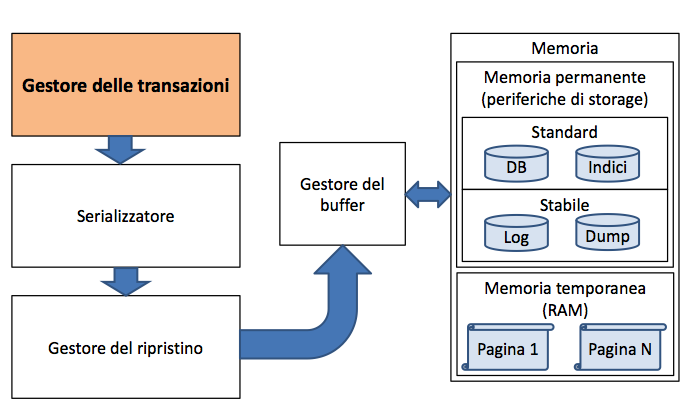
\includegraphics[scale = 0.45]{05/img01}
        \caption{Architettura dei DBMS}
    \end{figure}
    
    
Il \textbf{gestore delle transazioni} riceve le transazioni e ne gestisce il ciclo di vita inviando i comandi DML alle componenti sottostanti che devono eseguire l'azione richiesta.\\\\
Il \textbf{serializzatore} è responsabile della proprietà di \textit{isolamento} (quando il programmatore progetta una transazione, lo fa nell'ipotesi che il DBMS la esegua in modo isolato rispetto alle altre transazioni).\\\\
Il \textbf{gestore del ripristino}, oltre a gestire il ripristino in seguito a guasti, è responsabile della proprietà di \textit{atomicità} (la transazione dev'essere eseguita interamente o per nulla).\\
Il gestore del ripristino garantisce anche l'\textit{integrità} dei dati (se i dati vengono corrotti, il gestore del ripristino cerca di recuperare il dato corretto oppure forza un abort della transazione).\\\\
Il \textbf{gestore del buffer} è responsabile della \textbf{durabilità} (persistenza dei dati del DBMS).\\\\
La \textbf{consistenza} è di competenza sia del \textbf{gestore delle transazioni} (verifica di tutti i vincoli della base di dati) che del serializzatore.

\section{Memoria centrale}
Consideriamo la nostra area di lavoro, cioè la memoria centrale.\\
Nell'area di lavoro abbiamo la transizione $T_i$ che richiede la lettura/modifica di un record. Quando una transizione richiede l'attività su un record, invia delle richieste al gestore del buffer.\\
La transazione $T_i$ invia una richiesta chiamata \textbf{fix pid}, che significa: la transazione ha bisogno di avere a disposizione una pagina dati di indirizzo \textbf{pid}.

\subsection{Le pagine}
Tutti i dati del database (tabelle, indici, log e dump) sono organizzati in pagine.\\
Le pagine hanno dimensioni che dipendono dal sistema (anche variabili), e contengono i record.\\
Se la transazione ha bisogno di lavorare su un ben determinato record (tupla), bisogna cercare una pagina con un certo indirizzo \textbf{pid} che si presume contenga il record desiderato.

\subsubsection{Caricamento delle pagine}
La transazione per lavorare su un dato ha sempre bisogno di chiedere al buffer la disponibilità di una precisa pagina:
    \begin{enumerate}
        \item{Il \textbf{gestore del buffer} caricherà la pagina nel buffer stesso, prendendola dalla periferica di storage se non già presente nel buffer.}
        \item{Il gestore del buffer prende i dati memorizzati nel disco (settori di tracce sul disco) e li mette nella cache presente nella periferica stessa.}
        \item{Dalla cache vengono poste nel buffer della memoria centrale.}
        \item{Il gestore del buffer risponde alla transazione inviandole l'indirizzo della memoria centrale in cui trovare la pagina.}
        \item{La transazione acquisisce, tramite il comando \textbf{fix pid}, il puntatore alla zona di memoria (buffer) che contiene la pagina.}
        \item{In caso di lettura, si accontenta di leggere i dati.}
        \item{In caso di scrittura o modifica, avviene il processo inverso, ovvero, la transazione modifica i dati \textit{nel buffer}.}
        \item{È il gestore del buffer che si occupa di copiare la pagina con le modifiche nella periferica.}
    \end{enumerate}

\subsubsection{Semplificazione}
La pagina è composta da un certo numero di blocchi fisici, che a loro volta sono composti da un certo numero di settori.\\
In questo corso, però, confonderemo il blocco fisico con la pagina (dimensione blocco = dimensione pagina).\\\\
Le dimensioni caratteristiche dei blocchi fisici vanno dai 512 Byte ai 4KB, mentre le dimensioni delle pagine vanno dai 4KB agli 8KB.\\
Il dimensionamento della pagina è importante perché influisce sulle prestazioni dell'intero DBMS.

\subsubsection{Tempi di trasferimento}
Ricordiamo che i tempi di trasferimento di una pagina tra periferiche di storage e RAM (e viceversa) sono dell'ordine dei millisecondi ($10^{-3} s$).\\
I tempi di trasferimento di pagine in RAM sono dell'ordine dei nanosecondi ($10^{-9}$ s).\\\\
Il fattore di differenza è $10^6$: dunque, il costo temporale è tutto sulla movimentazione delle pagine dalla periferica alla memoria centrale (e viceversa).\\\\
Nonostante i progressi tecnologici, il divario ha ancora lo stesso ordine di grandezza.

\subsubsection{Struttura di una pagina}
La pagina contiene:
    \begin{itemize}
        \item{\textbf{Array degli offset}}
        \item{\textbf{Contatore CP}: conta i programmi che hanno avuto l'OK di accesso alla pagina}
        \item{\textbf{Set Dirty Bit}: vale 1 se la pagina è stata modificata.}
        \item{\textbf{Stack dei records}: ontenuto della pagina.}
        \item{\textbf{Bit di parità}}
    \end{itemize}
Per l'identificazione di un record è necessario fornire due valori:
    $$RID[PID, i]$$
Dove $PID$ è l'identificatore della pagina, mentre $i$ è un offset.\\
L'architettura di $RID$, con indice e offset, consente al gestore delle pagine (il filesystem) di modificare la posizione dei records a piacimento all'interno dell'area dati senza influenzare gli indirizzi esterni.

\part{SQL}
\chapter{Introduzione}

Il linguaggio SQL è il linguaggio di riferimento per tutti i DBMS relazionali, e implementa sia il DDL (Data Definition Language) che il DML (Data Manipulation Language).\\\\
SQL è un linguaggio che ci permette di interrogare e gestire le basi di dati.\\
Ciascuna interrogazione è implementata per mezzo di costrutti di programmazione detti \textbf{query}.\\\\
Per il linguaggio SQL sono stati realizzati diversi standard e diverse implementazioni.

\section{PostgreSQL}
PostgreSQL è un DBMS opensource, conforme agli standard SQL, che aggiunge ai database relazionali caratteristiche che lo rendono classificabile come object-relational.\\
Aggiunge inoltre funzionalità quali vincoli, trigger e rules.\\\\
PostgreSQL è basato su un'architettura Client/Server, ovvero la connessione è frutto di due processi:
    \begin{itemize}
        \item{Il processo \textbf{server}, chiamato postgres o postmaster, che accetta le connessioni dai client e ha il compito di interagire con i database su delega del client che ha fatto richiesta. Spesso gira su un altro computer, più potente, e accetta richieste contemporaneamente da più client.}
        \item{Un \textbf{client} che richiede di effettuare determinate operazioni su uno o più database. Un client può essere: un’applicazione grafica, una pagina web, un programma scritto da un utente. pgAdmin, l'utility che permette di impartire comandi SQL interattivamente, è un esempio di client.}
    \end{itemize}

\section{Domini dei dati}
\subsection{Caratteri e stringhe}
Le \textbf{stringhe a lunghezza fissa} vengono dichiarate con la seguente sintassi:
    \begin{lstlisting}{Stringhe}
        char(length)
    \end{lstlisting}
Le \textbf{stringhe a lunghezza variabile} vengono dichiarate con la seguente sintassi:
    \begin{lstlisting}{Stringhe}
        varchar(length)
    \end{lstlisting}
Quando la lunghezza di una stringa non viene specificata, si assume che sia 1 (\textbf{singolo carattere}).\\\\
\textbf{Esempi}:
    \begin{itemize}
        \item{$char(100)$: stringa di esattamente 100 caratteri}
        \item{$varchar(100)$: stringa di lunghezza variabile fino a un massimo di 100 caratteri}
        \item{$char$: un singolo carattere}
    \end{itemize}
    
\subsection{Tipi numerici esatti}
I numeri decimali vengono rappresentati in maniera esatta con una delle seguenti sintassi:
    \begin{lstlisting}{Numeri decimali}
        decimal (precisione, scala)
        numeric (precisione, scala)
   \end{lstlisting}
    \begin{itemize}
        \item{$precisione$: numero totale di cifre decimali (opzionale). Per $decimal$ la precisione specificata è quella minima garantita, per $numeric$ è quella esatta.}
        \item{$scala$: numero di cifre decimali dopo la virgola (opzionale).}
    \end{itemize}
I numeri interi vengono rappresentati con una delle seguenti sintassi:
    \begin{lstlisting}{Numeri interi}
        integer
        smallint
    \end{lstlisting}
La rappresentazione dei numeri interi è dipendente dalla specifica implementazione.\\\\
\textbf{Esempi}:
    \begin{itemize}
        \item{$decimal(6,4)$: decimali da -99.9999 a +99.999}
        \item{$numeric(4)$: decimali da -9999 a +9999}
        \item{$integer$: interi a 32 bit (solitamente)}
    \end{itemize}

\subsection{Tipi numerici approssimati}
I numeri in virgola mobile con mantissa ed esponente vengono rappresentati con la seguente sintassi:
    \begin{lstlisting}{Numeri approssimati}
        float (precisione)
        real
        double precision
    \end{lstlisting}
    \begin{itemize}
        \item{$precisione$: numero di cifre binarie per la mantissa}
    \end{itemize}

\subsection{Date}
Possiamo usare la seguente sintassi per rappresentare istanti temporali:
    \begin{itemize}
        \item{$date$: per le date. Comprende i sottocampi $year$, $month$, $day$.}
        \item{$time(precisione)$: per gli orari. Comprende i sottocampi $hour$, $minute$, $second$.}
        \item{$timestamp(precisione)$: per specificare sia date che orari. Comprende i sottocampi $year$, $month$, $day$, $hour$, $minute$, $second$.}
    \end{itemize}
    \begin{itemize}
        \item{$precisione$: numero di cifre per le frazioni di secondo (opzionale)}
    \end{itemize}
\textbf{Esempi}:
    \begin{itemize}
        \item{$timestamp(2)$: per memorizzare eventi di log con precisione al centesimo di secondo.}
    \end{itemize}
    
\subsection{Intervalli}
Per rappresentare gli intervalli temporali, usiamo la sintassi:
    \begin{lstlisting}{Intervalli Temporali}
        interval unita1 [to unita2]
    \end{lstlisting}
    \begin{itemize}
        \item{$unita1$: unità di tempo più grossolana}
        \item{$unita2$ (opzionale): unità di tempo più fine}
    \end{itemize}
\textbf{Esempi}:
    \begin{itemize}
        \item{$interval$ $year$: esprime intervalli in anni.}
        \item{$interval$ $year$ $to$ $month$: esprime intervalli misurati in anni e mesi (e.g. un anno e due mesi).}
        \item{$interval$ $day$ $to$ $second(2)$: esprime intervalli misurati in giorni, ore, minuti, secondi e centesimi di secondo.}
        \item{$interval$ $year$ $to$ $minute$: non è permesso (non si può passare in modo preciso da $month$ a $day$ perché i mesi hanno durata diversa.}
    \end{itemize}

\subsection{Altri domini}
    \begin{itemize}
        \item{$boolean$: valori booleani.}
        \item{$bigint$: interi "grossi"}
        \item{$blob$: Binary Large OBject (immagini, video, file di vario tipo) (in PostgreSQL $bytea$ oppure $lo$).}
        \item{$clob$: Character Large OBject (lunghi file di testo) (in PostgreSQL $text$).}
    \end{itemize}

\subsection{Domini personalizzati}
È possibile creare domini personalizzati (le parti tra $[]$ sono opzionali:
    \begin{lstlisting}{Domini personalizzati}
        create domain NomeDominio as TipoDato
        [default ValoreDefault] [Vincoli]
    \end{lstlisting}
    \begin{itemize}
        \item{$NomeDominio$: nome del nuovo dominio}
        \item{$TipoDato$: nome del tipo di base}
        \item{$default \quad ValoreDefault$: valore asseegnato in automatico, se non specificato esplicitamente (opzionale)}
        \item{$Vincoli$: insieme di vincoli sui valori assunti dal dominio personalizzato (opzionale)}
    \end{itemize}
I domini personalizzati sono comunque semplici (no array, no struct, no record).\\\\
\textbf{Esempio 1}: voto di un esame
    \begin{lstlisting}{Domini personalizzati - Esempio 1}
        create domain Voto
        as smallint default NULL
        check (value >= 18) AND (value <= 30);
    \end{lstlisting}
\textbf{Esempio 2}: temperatura corporea (gradi Celsius)
    \begin{lstlisting}{Domini personalizzati - Esempio 2}
        create domain Temperatura
        as decimal(3, 1) default NULL
        check (value >= 35) AND (value <= 42);
    \end{lstlisting}
L'utilità dei nuovi domini è legata alla possibilità di astrazione.\\\\
\textbf{Esempio 3}: per passare dai gradi Celsius ai gradi Fahrenheit è sufficiente cambiare una volta per tutte il dominio di Temperatura:
    \begin{lstlisting}{ Domini personalizzati - Esempio 3}
        create domain Temperatura
        as decimal(4, 1) default NULL
        check (value >= 95) AND (value <= 107.6);
    \end{lstlisting}

\section{Definizione di tabelle}
Per creare e definire una nuova tabella utilizziamo la seguente sintassi:
    \begin{lstlisting}{Creare nuova tabella}
        create table NomeTabella(
            NomeAttributo1 Dominio1 [ValoreDefault1][Vincoli1]
            ...
            Nome AttributoN DominioN [ValoreDefaultN][VincoliN]
        );
    \end{lstlisting}
\textbf{Esempio}: $Dipartimento(\underline{Nome}, Indirizzo, Citta)$
    \begin{lstlisting}{Esempio Dipartimento}
        create table Dipartimento(
            Nome varchar(20) primary key,
            Indirizzo varchar(50),
            Citta varchar(20) not null
        );
    \end{lstlisting}
    
\subsection{Valori di default}
Per ogni attributo può essere specificato un valore predefinito che verrà usato se, nell'inserimento di una riga, non viene specificato un valore per quell'attributo.\\\\
\textbf{Esempio}: 
    \begin{lstlisting}{Esempio Valori Default}
        NumeroFigli smallint default 0,
        Email varchar(64) default 'unito.it',
        StatoCivile varchar(20) default 'libero'
    \end{lstlisting}
Se non si specifica esplicitamente un valore di default, viene usato $null$.

\section{Definizione dei vincoli}
I vincoli servono a definire proprietà che devono essere verificate da ogni istanza della base di dati per garantirne l'integrità (vincoli di integrità).\\
Si differenziano in:
    \begin{itemize}
        \item{\textbf{Vincoli intrarelazionali}: relativi a una sola tabella}
        \item{\textbf{Vincoli interrelazionali}: relativi a più tabelle}
    \end{itemize}
Si possono specificare:
    \begin{itemize}
        \item{Contestualmente alla definizione degli attributi}
        \item{Alla fine della definizione della tabella}
    \end{itemize}
Si possono usare vincoli predefiniti oppure si può specificare l'espressione logica che il vincolo deve verificare.\\\\
In alcune occasioni può essere utile assegnare un nome a un vincolo. Per farlo si utilizza la seguente sintassi dopo tutte le definizioni di attributi:
    \begin{lstlisting}
        constraint NomeVincolo DefinizioneVincolo
    \end{lstlisting}

\subsection{Vincoli intrarelazionali predefiniti}
\textbf{Vincolo $not$ $null$:}
    \begin{itemize}
        \item{È un vincolo di tupla che indica che il valore nullo non è ammesso come valore per un determinato attributo, quindi rende l'attributo obbligatorio}
        \item{Se l'attributo non viene specificato in fase di inserimento e non si è specificato un valore di default, si viola il vincolo d'integrità e l'operazione è annullata}
        \item{Sintassi
            \begin{lstlisting}
                NomeAttributo Dominio {}not null
            \end{lstlisting}}
        \item{Se per l'attributo viene specificato un valore di default è possibile effettuare l'inserimento anche senza specificarne il valore.}
    \end{itemize}
\textbf{Esempio}
    \begin{lstlisting}
        Citta varchar(20) not null
    \end{lstlisting}
    
\textbf{Vincolo $unique$:}
    \begin{itemize}
        \item{È un vincolo di tabella che indica che il valore di un attributo o le combinazioni di valori su un insieme di attributi sono una superchiave:
            $$righe \text{ } diverse \leftrightarrow 
            valori \text{ } diversi$$}
        \item{Fa eccezione il valore nullo (che può comparire in più righe senza violare il vincolo).}
        \item{Sintassi (vincolo su un solo attributo):
            \begin{lstlisting}
                NomeAttributo Dominio unique
            \end{lstlisting}}
    \end{itemize}
\textbf{Esempio}
    \begin{lstlisting}
        Matricola varchar(6) unique
    \end{lstlisting}
    
\textbf{Vincolo $unique$ su insiemi di attributi}:
    \begin{itemize}
        \item{Va specificato dopo la definizione degli attributi della tabella.}
        \item{Sintassi:
            \begin{lstlisting}
                NomeAttributo1 Dominio1
                NomeAttributo2 Dominio2
                ...
                unique (NomeAttributo1, NomeAttributo2)
            \end{lstlisting}}
    \end{itemize}
\textbf{Esempio}
    \begin{lstlisting}
        Nome varchar(255),
        Cognome varchar(255),
        unique(Nome, Cognome)
    \end{lstlisting}
    
\textbf{Vincolo $primary$ $key$ di chiave primaria}:
    \begin{itemize}
        \item{È un vincolo di tabella che indica che un attributo o un insieme di attributi sono la chiave primaria.}
        \item{Gli attributi così definiti non possono assumere valore nullo.}
        \item{Può esserci un solo vincolo primary key per ogni tabella.}
        \item{Vincolo $primary$ $key$ su un solo attributo: va specificato nella definizione dell'attributo mediante la seguente sintassi:
            \begin{lstlisting}
                NomeAttributo Dominio primary key
            \end{lstlisting}}
        \item{Vincolo $primary$ $key$ su un insieme di attributi: va specificato dopo la definizione degli attributi mediante la seguente sintassi:
            \begin{lstlisting}
                NomeAttributo1 Dominio1,
                NomeAttributo2 Dominio2,
                ...
                primary key (NomeAttributo1, NomeAttributo2, ...)
            \end{lstlisting}}
    \end{itemize}

\subsubsection{Vincoli interrelazionali predefiniti}
Un \textbf{vincolo di integrità referenziale} (di \textbf{chiave esterna}):
    \begin{itemize}
        \item{Crea un vincolo tra i valori uno o più attributi della tabella (interna) su cui è definito e uno o più attributi di un'altra tabella (esterna).}
        \item{Per ogni riga della tabella interna, il valore dell'attributo specificato nel vincolo, se diverso da $null$, dev'essere presente tra i valori del corrispondente attributo della tabella esterna.}
        \item{Sintassi con un solo attributo:
            \begin{lstlisting}
                NomeAttributo references NomeTabellaEsterna(NomeAttributoEsterno)
            \end{lstlisting}}
        \item{Sintassi con più attributo:
            \begin{lstlisting}
                NomeAttributo1 Dominio1,
                NomeAttributo2 Dominio2,
                ...
                foreign key (NomeAttributo1, NomeAttributo2, ...)
                    references NomeTabellaEsterna (NomeAttributoEsterno1, Nome AttributoEsterno2, ...)
            \end{lstlisting}
            L'ordine è importante! Ciascun attributo viene mappato al corrisponente secondo l'ordine con cui lo specifichiamo.}
    \end{itemize}

\subsubsection{Violazione del vincolo di integrità referenziale}
In generale, quando un vincolo viene violato, il DBMS rifiuta l'operazione che causerebbe la violazione e segnala un errore.\\
Con i vincoli di integrità referenziale si possono specificare altre reazioni da adottare in caso di violazione.\\\\
Casi in cui può avvenire una violazione di un vincolo di integrità referenziale:
    \begin{enumerate}
        \item{Inserimento di una nuova riga nella tabella interna.}
        \item{Modifica, nella tabella interna, di un valore dell'attributo referente.}
        \item{Modifica, nella tabella esterna, di un valore dell'attributo riferito.}
        \item{Cancellazione di una riga nella tabella esterna.}
    \end{enumerate}
I primi due casi riguardano un cambiamento della \textbf{tabella interna}, gli ultimi due un cambiamento della \textbf{tabella esterna}.\\\\
Quando cambia la tabella interna (casi 1 e 2), l'operazione viene semplicemente \textbf{rifiutata}.\\
Quando cambia la tabella esterna (casi 3 e 4), si può specificare quali variazioni apportare alla tabella interna.\\
Questa asimmetria nel comportamento deriva dal fatto che dal punto di vista applicativo la tabella esterna ricopre il ruolo di tabella principale (\textbf{master}) e quella interna di secondaria (\textbf{slave}) che deve adeguarsi alle variazioni.\\\\
In seguito a una \textbf{modifica} (caso 3), le reazioni possono essere le seguenti:
    \begin{enumerate}
        \item{\textbf{cascade}: il nuovo valore dell'attributo della tabella esterna viene riportato in tutte le corrispondenti righe della tabella interna.}
        \item{\textbf{set null}: all'attributo referente viene assegnato il valore nullo al posto del valore modificato nella tabella esterna.}
        \item{\textbf{set default}: all'attributo referente viene assegnato il valore di default al posto del valore modificato nella tabella esterna.}
        \item{\textbf{no action}: nessuna reazione (e quindi la modifica non viene consentita).}
    \end{enumerate}
In seguito a una \textbf{cancellazione} (caso 4), le reazioni possono essere le seguenti:
    \begin{enumerate}
        \item{\textbf{cascade}: tutte le righe della tabella interna corrispondenti alla riga cancellata nella tabella esterna vengono cancellate.}
        \item{\textbf{set null}: all'attributo referente viene assegnato il valore nullo al posto del valore cancellato nella tabella esterna.}
        \item{\textbf{set default}: all'attributo referente viene assegnato il valore di default al posto del valore cancellato nella tabella esterna.}
        \item{\textbf{no action}: nessuna reazione (e quindi la cancellazione non viene consentita).}
    \end{enumerate}
La sintassi per specificare il comportamento in caso di violazione di un vincolo interrelazionale è la seguente:
    \begin{lstlisting}
        //Per la modifica, subito dopo il vincolo
        on update Reazione
        //Per la cancellazione, subito dopo il vincolo
        on delete Reazione
    \end{lstlisting}

\subsubsection{Esempio}
    \begin{lstlisting}{Creazione tabella Ricoveri}
        create table Ricoveri (
            PAZ varchar(4),
            Inizio date,
            Fine date,
            Reparto char,
            primary key (PAZ, Inizio),
            foreign key (PAZ) references Pazienti(COD)
                on update cascade
                on delete no action,
            foreign key (Reparto) references Reparti (COD)
                on update cascade
                on delete set null
        );
    \end{lstlisting}

\section{Modifiche alle definizioni}
SQL permette di modificare la definizione di tabelle, domini, vincoli precedentemente introdotti:
    \begin{lstlisting}{Modifica definizioni}
        alter (modifica),
        drop (cancellazione),
        add (aggiunta)
    \end{lstlisting}

\chapter{Query di Base}

Le operazioni di interrogazione in SQL vengono specificate per mezzo dell'istruzione \texttt{select}.\\
Vediamone la struttura essenziale:
    \begin{lstlisting}
        select Attributo1 [[as] AliasAttributo1]...
        from Tabella1 [[as] AliasTabella1], ...
        [where Condizione]
    \end{lstlisting}
Le tre parti di cui si compone un'istruzione \texttt{select} vengono spesso chiamate:
    \begin{itemize}
        \item{Clausola \texttt{select}}
        \item{Clausola \texttt{from}}
        \item{Clausola \texttt{where}}
    \end{itemize}
L'interrogazione SQL seleziona, tra le righe che appartengono al prodotto cartesiano delle tabelle elencate nella clausola \texttt{from}, quelle che soddisfano le condizioni espresse nell'argomento della clausola \texttt{where}.\\
Il risultato dell'esecuzione di un'interrogazione SQL è quindi una tabella con una riga per ogni riga prodotta dalla clausola \texttt{from} e filtrata dalla clausola \texttt{where}, le cui colonne si ottengono dalla valutazione delle espressioni che appaiono nella clausola \texttt{select}.\\
Ogni colonna viene eventualmente ridenominata con l'\texttt{Alias} specificato.

\subsubsection{Esempio 1}
Consideriamo la seguente base dati:
    \begin{equation}\begin{aligned}
        IMPIEGATO (\underline{Nome, Cognome}, Dipartimento, Ufficio, Stipendio, Citta)\\
        DIPARTIMENTO (\underline{Nome}, Indirizzo, Citta)
    \end{aligned}\end{equation}
Estrarre lo stipendio degli impiegati di cognome "Rossi":
    \begin{lstlisting}{Esempio 1}
        select 
            Stipendio as Salario
        from 
            Impiegato
        where 
            Cognome = 'Rossi'
    \end{lstlisting}
Se non vi sono impiegati di cognome "Rossi", l'interrogazione restituirà un insieme vuoto, altrimenti, un insieme con tante righe quanti sono tali impiegati. 


\section{Clausola \texttt{select}}
La clausola \texttt{select} specifica gli elementi dello schema della tabella risultato.\\
Come argomento della \texttt{select} può anche comparire il carattere speciale $*$, che rappresenta la selezione di tutti gli attributi delle tabella indicate nelle \texttt{from}.\\\\
Inoltre, nella \texttt{select} possono comparire generiche espressioni sul valore degli attributi di ciascuna riga selezionata.

\subsubsection{Esempio 2}
Consideriamo la seguente base dati:
    \begin{equation}\begin{aligned}
        IMPIEGATO (\underline{Nome, Cognome}, Dipartimento, Ufficio, Stipendio, Citta)\\
        DIPARTIMENTO (\underline{Nome}, Indirizzo, Citta)
    \end{aligned}\end{equation}
Estrarre tutte le informazioni relative agli impiegati di cognome "Rossi"
    \begin{lstlisting}{Esempio 2}
        select *
        from 
            Impiegato
        where 
            Cognome = 'Rossi'
    \end{lstlisting}

\subsubsection{Esempio 3}
Consideriamo la seguente base dati:
    \begin{equation}\begin{aligned}
        IMPIEGATO (\underline{Nome, Cognome}, Dipartimento, Ufficio, Stipendio, Citta)\\
        DIPARTIMENTO (\underline{Nome}, Indirizzo, Citta)
    \end{aligned}\end{equation}
Estrarre lo stipendio mensile dell'impiegato che ha cognome "Bianchi"
    \begin{lstlisting}{Esempio 3}
        select 
            Stipendio/12 as StipendioMensile
        from 
            Impiegato
        where 
            Cognome = 'Bianchi'
    \end{lstlisting}



\section{Clausola \texttt{from}}
Quando si desidera formulare un'interrogazione che coinvolge righe appartenenti a più di una tabella, si pone come argomento della \texttt{from} l'insieme di tabelle alle quali si vuole accedere. Sul prodotto cartesiano delle tabelle elenecate verranno poi applicate le condizioni della \texttt{where}.\\
Quindi, un join può essere specificato indicando in modo esplicito le condizioni che esprimono il legame tra le diverse tabelle.\\
Quando abbiamo a che fare con più tabelle, può accadere che compaiano attributi omonimi: in questo caso è possibile utilizzare gli alias oppure utilizzare la notazione "." specificando prima del punto la tabella da cui prendiamo l'attributo (\texttt{Tabella.Attributo}).

\subsubsection{Esempio 4}
Consideriamo la seguente base dati:
    \begin{equation}\begin{aligned}
        IMPIEGATO (\underline{Nome, Cognome}, Dipartimento, Ufficio, Stipendio, Citta)\\
        DIPARTIMENTO (\underline{Nome}, Indirizzo, Citta)
    \end{aligned}\end{equation}
Estrarre i nomi degli impiegati e le città in cui lavorano
    \begin{lstlisting}{Esempio 4}
        select 
            Impiegato.Nome,
            Impiegato.Cognome, 
            Dipartimento.Citta
        from 
            Impiegato, Dipartimento
        where 
            Impiegato.Dipartimento = Dipartimento.Nome
    \end{lstlisting}

\subsubsection{Esempio 5}
Consideriamo la seguente base dati:
    \begin{equation}\begin{aligned}
        IMPIEGATO (\underline{Nome, Cognome}, Dipartimento, Ufficio, Stipendio, Citta)\\
        DIPARTIMENTO (\underline{Nome}, Indirizzo, Citta)
    \end{aligned}\end{equation}
Estrarre i nomi degli impiegati e le città in cui lavorano utilizzando degli alias per le tabelle
    \begin{lstlisting}{Esempio 5}
        select 
            I.Nome, 
            I.Cognome, 
            D.Citta
        from 
            Impiegato as I, 
            Dipartimento as D
        where 
            I.Dipartimento = D.Nome
    \end{lstlisting}



\section{Clausola \texttt{where}}
La clausola \texttt{where} ammette come argomento un'espressione booleana costituita combinando predicati semplici con gli operatori $AND$, $OR$ e $NOT$.\\
Ciascun predicato utilizza gli operatori di confronto ($=, <>, <, <=, >, >=$) per confrontare da un lato un'espressione costruita a partire dai valori degli attributi per la riga, e dall'altro lato un valore costante o un'altra espressione.\\\\
La sintassi assegna la precedenza all'operatore $NOT$, ma non definisce una relazione di precedenza tra l'$AND$ e l'$OR$. Se è necessario esprimere un'interrogazione che richieda sia l'uso dell'$AND$ che del $NOT$, conviene esplicitare l'ordine di valutazione mediante le parentesi.\\\\
Oltre ai normali predicati di confronto, SQL mette a disposizione un operatore \texttt{like} per il confronto di stringhe, che permette di effettuare confronti con stringhe in cui compaiono caratteri speciali ($\_$) oppure $\%$.\\
Il carattere $\_$ rappresenta nel confronto un carattere arbitrario, mentre il carattere $\%$ rappresenta una stringa di un numero arbitrario (eventualmente nullo) di caratteri arbitrari.\\
Un confronto del tipo $\texttt{like} ab\%ba\_$ sarà soddisfatto da una qualunque stringa di caratteri che inizi con $ab$ e la stringa $ba$ prima dell'ultima posizione.

\subsubsection{Esempio 6}
Consideriamo la seguente base dati:
    \begin{equation}\begin{aligned}
        IMPIEGATO (\underline{Nome, Cognome}, Dipartimento, Ufficio, Stipendio, Citta)\\
        DIPARTIMENTO (\underline{Nome}, Indirizzo, Citta)
    \end{aligned}\end{equation}
Estrarre il nome e il cognome degli impiegati che lavorano nell'ufficio 20 del dipartimento $Amministrazione$
    \begin{lstlisting}{Esempio 6}
        select 
            I.Nome, 
            I.Cognome
        from 
            Impiegato as I
        where 
            I.Ufficio = 20
            and I.Dipartimento = 'Amministrazione'
    \end{lstlisting}
    
\subsubsection{Esempio 7}
Consideriamo la seguente base dati:
    \begin{equation}\begin{aligned}
        IMPIEGATO (\underline{Nome, Cognome}, Dipartimento, Ufficio, Stipendio, Citta)\\
        DIPARTIMENTO (\underline{Nome}, Indirizzo, Citta)
    \end{aligned}\end{equation}
Estrarre i nomi e i cognomi degli impiegati che lavorano al dipartimento $Amministrazione$ o al dipartimento $Produzione$.
    \begin{lstlisting}{Esempio 7}
        select 
            I.Nome,
            I.Cognome
        from 
            Impiegato as I
        where 
            I.Dipartimento = 'Amministrazione'
            or I.Dipartimento = 'Produzione'
    \end{lstlisting}
    
\subsubsection{Esempio 8}
Consideriamo la seguente base dati:
    \begin{equation}\begin{aligned}
        IMPIEGATO (\underline{Nome, Cognome}, Dipartimento, Ufficio, Stipendio, Citta)\\
        DIPARTIMENTO (\underline{Nome}, Indirizzo, Citta)
    \end{aligned}\end{equation}
Estrarre i nomi propri degli impiegati di cognome "Rossi" che lavorano al dipartimento $Produzione$ o $Amministrazione$.
    \begin{lstlisting}{Esempio 8}
        select 
            I.Nome
        from 
            Impiegato as I
        where 
            (I.Dipartimento = 'Produzione'
            or I.Dipartimento = 'Amministrazione)
            and I.Cognome = 'Rossi'
    \end{lstlisting}
    
\subsubsection{Esempio 9}
Consideriamo la seguente base dati:
    \begin{equation}\begin{aligned}
        IMPIEGATO (\underline{Nome, Cognome}, Dipartimento, Ufficio, Stipendio, Citta)\\
        DIPARTIMENTO (\underline{Nome}, Indirizzo, Citta)
    \end{aligned}\end{equation}
Estrarre gli impiegati che hanno un cognome che ha una $o$ in seconda posizione e finisce per $i$.
    \begin{lstlisting}{Esempio 9}
        select 
            I.Nome, I.Cognome
        from 
            Impiegato as I
        where 
            I.Cognome like '_o%i'
    \end{lstlisting}



\section{Gestione dei valori nulli}
Un valore nullo in un attributo può significare che tale attributo non è applicabile, o che il valore è applicabile ma non è conosciuto o anche che non si sa in quale delle due situazioni ci troviamo.\\
Per selezionare i termini con valori nulli, SQL fornisce il predicato \texttt{is null}, la cui sintassi è semplicemente
    $$\texttt{Attributo is [not] null}$$
Il predicato risulta vero solo se l'attributo ha valore nullo, mentre il predicato \texttt{is not null} è la sua negazione.\\\\
I valori nulli hanno un particolare impatto sulla valutazione dei normali predicati.\\
Consideriamo un semplice predicato di confronto fra un attributo della tabella $T$ e un valore costante:
    $$\texttt{A > c}$$
Questo predicato sarà vero per le righe in cui l'attributo $A$ è superiore a $c$.\\
Osserviamo che ci sono due soluzioni per gestire il caso in cui $A$ sia nullo: la prima soluzione, più immediata, usa la \textbf{logica a due valori} e prevede semplicemente di considerare falso il predicato.\\
La seconda soluzione, quella adottata in SQL a partire da SQL-2, fa uso di una \textbf{logica a tre valori}, in cui un predicato semplice restituisce il valore $unknown$ quando uno qualsiasi dei suoi termini ha valore nullo. Fa eccezione, ovviamente, il predicato \texttt{is null}, che restituisce sempre o vero o falso.\\
La differenza tra le soluzioni basate sulle logiche a due e tre valori emerge solo quando si valutano espressioni complicate. In alcuni casi il comportamento del sistema in presenza di valori nulli può diventare molto poco intuitivo, richiedendo una maggiore attenzione.



\section{Duplicati}
Una significativa differenza tra SQL e algebra relazionale è data dalla gestione dei duplicati. Mentre in algebra una tabella viene vista come una relazione dal punto di vista matematico, e quindi come un insieme di elementi (tuple) diversi tra loro, in SQL si possono avere in una tabella più righe uguali (dette duplicati), ovvero righe con gli stessi valori su tutti gli attributi.\\\\
Per emulare il comportamento dell'algebra relazionale, sarebbe necessario efettuare l'eliminazione dei duplicati tutte le volte che si eseguono operazioni di proiezione. L'operazione di eliminazione di duplicati, però, è molto costosa, e spesso non è necessaria, in quanto in molti casi il risultato non contiene duplicati.\\
Per esempio, quando il risultato include una chiave per ogni tabella che compare nella \texttt{from}, la tabella risultato non può contenere più esemplari della stessa riga. Per questo in SQL si è stabilito di permettere la presenza di duplicati all'interno delle tabelle, lasciando al programmatore il compito di specificare esplicitamente quando l'operazione di rimozione di duplicati è necessaria.\\\\
L'eliminazione dei duplicati è specificata con la parola chiave \texttt{distinct}, da porre immediatamente dopo la parola chiave \texttt{select}.\\
La sintassi prevede che si possa anche specificare la parola chiave \texttt{all} al posto di \texttt{distinct}, indicando che si intendono mantenere tutti i duplicati. L'indicazione della parola \texttt{all} è opazionale, in quanto, come già detto, il mantenimento dei duplicati costituisce l'opzione di default.

\subsubsection{Esempio 10}
Consideriamo la seguente base dati:
    \begin{equation}\begin{aligned}
        IMPIEGATO (\underline{Nome, Cognome}, Dipartimento, Ufficio, Stipendio, Citta)\\
        DIPARTIMENTO (\underline{Nome}, Indirizzo, Citta)
    \end{aligned}\end{equation}
Estrarre gli impiegati di cognome "Rossi" che abitano nella stessa città, presentando eventualmente più volte lo stesso valore di \texttt{Citta}.
    \begin{lstlisting}{Esempio 10}
        select 
            I.Citta
        from 
            Impiegato as I
        where 
            I.Cognome = 'Rossi'
    \end{lstlisting}
    
\subsubsection{Esempio 11}
Consideriamo la seguente base dati:
    \begin{equation}\begin{aligned}
        IMPIEGATO (\underline{Nome, Cognome}, Dipartimento, Ufficio, Stipendio, Citta)\\
        DIPARTIMENTO (\underline{Nome}, Indirizzo, Citta)
    \end{aligned}\end{equation}
Estrarre gli impiegati di cognome "Rossi" che abitano nella stessa città, facendo comparire al più una volta ogni città.
    \begin{lstlisting}{Esempio 11}
        select distinct
            I.Citta
        from 
            Impiegato as I
        where 
            I.Cognome = 'Rossi'
    \end{lstlisting}



\section{Uso di variabili}
Abbiamo già visto come nelle interrogazioni SQL sia possibile associare un nome alternativo, detto $alias$, alle tabelle che compaiono come argomento della clausola \texttt{from}.\\
Il nome viene usato per far riferimento alla tabella nel contesto dell'interrogazione. Questa funzionalità può essere sfruttata per far riferimento a una tabella in modo compatto, ricorrendo a brevi alias ed evitando così di scrivere per esteso il nome della tabella tutte le volte che ne viene richiesto l'uso. Vi sono, però, altre ragioni per utilizzare gli alias.\\\\
Per prima cosa, utilizzando gli alias è possibile fare accesso più volte alla stessa tabella, come avviene nel calcolo relazionale quando si usano più variabili associate alla stessa tabella e in modo simile all'uso dell'operatore di ridenominazione $\rho$ dell'algebra relazionale.\\
Tutte le volte che si introduce un alias per una tabella si dichiara in effetti una variabile che rappresenta le righe della tabella di cui è alias. Quando una tabella compare una sola volta in un'interrogazione, non c'è differenza tra l'interpretare l'alias come uno pseudonimo o come una nuova variabile. Quando una tabella compare invece più volte, è necessario considerare l'alias come una nuova variabile.

\subsubsection{Esempio 12}
Consideriamo la seguente base dati:
    \begin{equation}\begin{aligned}
        IMPIEGATO (\underline{Nome, Cognome}, Dipartimento, Ufficio, Stipendio, Citta)\\
        DIPARTIMENTO (\underline{Nome}, Indirizzo, Citta)
    \end{aligned}\end{equation}
Estrarre tutti gli impiegati che hanno lo stesso cognome (ma diverso nome) di impiegati dipartimento $Produzione$.
    \begin{lstlisting}{Esempio 12}
        select distinct
            I1.Nome,
            I1.Cognome
        from 
            Impiegato as I1
            Impiegato as I2
        where 
            I1.Cognome = I2.Cognome
            and I1.Nome <> I2.Nome
            and I2.Dipartimento = 'Produzione'
    \end{lstlisting}
Questa interrogazione confronta ciascuna riga di $IMPIEGATO$ con tutte le righe di $IMPIEGATO$ associate al dipartimento $Produzione$. \\
Si osservi che in questa interrogazione ogni riga con $Produzione$ come valore dell'attributo $Dipartimento$ viene confrontata anche con se stessa, ma il confronto della riga con se stessa non sarà mai soddisfatto, in quanto il predicato di disuguaglianza sull'attributo $Nome$ non potrà mai essere vero.\\
Per illustrare l'esecuzione di quest'interrogazione si può immaginare che al momento della definizione degli alias, vengano create due diverse tabelle associate alle variabili $I1$ e $I2$, ciascuna con tutte le righe di $IMPIEGATO$; ciascuna variabile assumerà quindi ciascun valore di tupla in modo indipendente dell'altra variabile.




\section{Ordinamento}
Mentre una relazione è costituita da un insieme non ordinato di tuple, nell'uso reale delle basi di dati sorge spesso il bisogno di costruire un ordine sulle righe delle tabelle.\\
SQL permette di specificare un ordinamento delle righe del risultato di un'interrogazione tramite la clausola \texttt{order by}, con la quale si chiude l'interrogazione. La clausola rispetta la seguente sintassi:
    $$\texttt{order by AttributoDiOrdinamento1 [asc|desc] {, AttributodiOrdinamento2 [asc|desc]}}$$
In questo modo si specificano gli attributi che devono essere utilizzati per l'ordinamento: per prima cosa le righe vengono ordinate in base al primo attributo nell'elenco; per righe che hanno lo stesso valore sul primo attributo, si considerano i valori degli attributi successivi, in sequenza.\\
L'ordine su ciascun attributo può essere ascendente o discendente, a seconda che si sia usato il quantificatore \texttt{asc} o \texttt{desc}. Se il quantificatore è omesso, so assume un ordinamento ascendente.

\subsubsection{Esempio 13}
Consideriamo la seguente base dati:
    \begin{equation}\begin{aligned}
        IMPIEGATO (\underline{Nome, Cognome}, Dipartimento, Ufficio, Stipendio, Citta)\\
        DIPARTIMENTO (\underline{Nome}, Indirizzo, Citta)
    \end{aligned}\end{equation}
Estrarre i nomi propri di tutti gli impiegati del dipartimento $Produzione$ ordinati in ordine decrescente.
    \begin{lstlisting}{Esempio 13}
        select distinct
            I.Nome
        from 
            Impiegato as I
        where 
            I.Dipartimento = 'Produzione'
        orderby I.Nome desc
    \end{lstlisting}
\chapter{Join}

Abbiamo visto come specificare il join attraverso una clausola \texttt{where} sul prodotto cartesiano.\\
SQL implementa anche una sintassi più immediata, attraverso l'utilizzo della parola chiave \texttt{join}.
    \begin{lstlisting}{Sintassi del join}
        select
        from
            Tabella1 [as Alias1]
            [TipoJoin] join 
            Tabella2 [as Alias2]
                on CondizioneJoin
        [where AltraCondizione]
    \end{lstlisting}
Mediante questa sintassi la condizione di join non compare come argomento della clausola \texttt{where}, ma viene invece spostata nell'ambito della clausola \texttt{from}, associata alle tabelle che vengono coinvolte nel join.\\\\
Il parametro \texttt{TipoJoin} specifica qual è il tipo di join da usare, e ad esso si possono sostituire i termini \texttt{inner, right outer, left outer, full outer} (il qualificatore \texttt{outer} è opzionale).\\\\
Con il join intenro le righe che vengono coinvolte nel join sono in generale un sottoinsieme delle righe di ciascuna tabella. Può, infatti, capitare che alcune righe non vengano considerate in quanto non esiste una corrispondente riga nell'altra tabella per cui la condizione sia soddisfatta. Questo comportamento spesso non rispetta le esigenze delle applicazioni, le quali, all'eliminazione delle righe operata dal join, possono preferire di mantenere le righe, introducendo dei valori nulli per rappresentare l'assenza di informazioni provenienti dall'altra tabella.\\\\
Il join esterno, invece, esegue un join mantenendo tutte le righe che fanno parte di una o entrambe le tabelle coinvolte.\\
Esistono tre varianti dei join esterni: \texttt{left}, \texttt{right} e \texttt{full}. Il \texttt{left join} fornisce come risultato il join esterno esteso con le righe della tabella che compare a sinistra per le quali non esiste una corrispondente riga nella tabella di destra.\\
Il \texttt{right join} si comporta in modo simmetrico (conserva le righe escluse della tabella di destra).\\
Infine, il \texttt{full join} restituisce il join interno esteso con le righe escluse di entrambe le tabelle.\\\\
Possiamo, inoltre, realizzare il \texttt{natural join} utilizzando nel join di due tabelle una condizione implicita di uguaglianza su tutti gli attributi caratterizzati dallo stesso nome.\\
Nonostante il vantaggio di una scrittura più compatta, il join naturale non è normalmente consigliabile (e spesso non è offerto dai sistemi commerciali). Un motivo è che un'interrogazione che usa il join naturale può introdurre dei rischi nelle applicazioni, in quanto il suo comportamento può mutare profondamente al variare dello schema delle tabelle.

\subsubsection{Esempio 1}
Consideriamo la seguente base dati:
    \begin{equation}\begin{aligned}
        IMPIEGATO (\underline{Nome, Cognome}, Dipartimento, Ufficio, Stipendio, Citta)\\
        DIPARTIMENTO (\underline{Nome}, Indirizzo, Citta)
    \end{aligned}\end{equation}
Estrarre i nomi degli impiegati e le città in cui lavorano utilizzando degli alias per le tabelle
    \begin{lstlisting}{Esempio 1}
        select 
            I.Nome, 
            I.Cognome, 
            D.Citta
        from 
            Impiegato as I
            join 
            Dipartimento as D
                on (I.Dipartimento = D.Nome)
    \end{lstlisting}
    
\subsubsection{Esempio 2}
Consideriamo la seguente base dati:
    \begin{equation}\begin{aligned}
        GUIDATORE (\underline{NroPatente}, Nome, Cognome)\\
        AUTOMOBILE (\underline{Targa}, Modello, NroPatente)
    \end{aligned}\end{equation}
Estrarre i guidatori con le automobili loro associate, mantenendo nel risultato anche i guidatori senza automobile
    \begin{lstlisting}{Esempio 2}
        select 
            G.Nome,
            G.Cognome
        from 
            Guidatore as G
            left join 
            Automobile as A
                on (G.NroPatente = A.NroPatente)
    \end{lstlisting}

\subsubsection{Esempio 3}
Consideriamo la seguente base dati:
    \begin{equation}\begin{aligned}
        GUIDATORE (\underline{NroPatente}, Nome, Cognome)\\
        AUTOMOBILE (\underline{Targa}, Modello, NroPatente)
    \end{aligned}\end{equation}
Estrarre tutti i guidatori e tutte le auto, mostrando tutte le relazioni esistenti tra di essi.
    \begin{lstlisting}{Esempio 3}
        select 
            G.Nome,
            G.Cognome, 
            G.NroPatente,
            A.Targa,
            A.Modello
        from 
            Guidatore as G
            full join 
            Automobile as A
                on (G.NroPatente = A.NroPatente)
    \end{lstlisting}
    
\subsubsection{Esempio 4}
Consideriamo la seguente base dati:
    \begin{equation}\begin{aligned}
        GUIDATORE (\underline{NroPatente}, Nome, Cognome)\\
        AUTOMOBILE (\underline{Targa}, Modello, NroPatente)
    \end{aligned}\end{equation}
Estrarre tutti i guidatori e tutte le auto, mostrando tutte le relazioni esistenti tra di essi.
    \begin{lstlisting}{Esempio 4}
        select 
            G.Nome,
            G.Cognome, 
            G.NroPatente,
            A.Targa,
            A.Modello
        from 
            Guidatore as G
            natural join 
            Automobile as A
    \end{lstlisting}

\chapter{Aggregati}




\section{Operatori aggregati}
Gli operatori aggregati costituiscono una delle più importanti estensioni di SQL rispetto all'algebra relazionale. Infatti, in algebra relazionale tutte le condizioni vengono valutate su una tupla alla volta, la condizione è sempre un predicato che viene valutato su ciascuna tupla indipendentemente da tutte le altre.\\
Spesso, però, nei contesti reali è richiesto di valutare delle proprietà che dipendono da insiemi di tuple.\\\\
Gli operatori aggregati vengono gestiti come un'estensione delle normali interrogazioni. Prima viene normalmente eseguita l'interrogazione, considerando solo le parti \texttt{from} e \texttt{where}.\\
L'operatore aggregato viene poi applicato alla tabella contenente il risultato dell'interrogazione.


\subsection{Operatore \texttt{count}}
L'operatore \texttt{count} calcola il numero di tuple che compongono la tabella risultante dall'interrogazione, usando la seguente sintassi:
    $$\texttt{count (<* | [distinct|all] listaAttributi>)}$$
La prima opzione \texttt{*} restituisce il numero di righe.\\
L'opzione \texttt{distinct} restituisce il numero di diversi valori degli attributi in \texttt{ListaAttributi}.\\
L'opzione \texttt{all} restituisce il numero di righe che possiedono valori diversi dal valore nullo per gli attributi in \texttt{ListaAttributi}.\\
Se si specifica un attributo e si omette \texttt{distinct} o \texttt{all}, si assume \texttt{all} come default.
    
\subsubsection{Esempio 1}
Consideriamo la seguente base dati:
    \begin{equation}\begin{aligned}
        IMPIEGATO (\underline{Nome, Cognome}, Dipartimento, Ufficio, Stipendio, Citta)\\
        DIPARTIMENTO (\underline{Nome}, Indirizzo, Citta)
    \end{aligned}\end{equation}
Estrarre il numero di impiegati del dipartimento $Produzione$
    \begin{lstlisting}{Esempio 1}
        select 
            count(*)
        from 
            Impiegato as I
        where 
            I.Dipartimento = 'Produzione'
    \end{lstlisting}

\subsubsection{Esempio 2}
Consideriamo la seguente base dati:
    \begin{equation}\begin{aligned}
        IMPIEGATO (\underline{Nome, Cognome}, Dipartimento, Ufficio, Stipendio, Citta)\\
        DIPARTIMENTO (\underline{Nome}, Indirizzo, Citta)
    \end{aligned}\end{equation}
Estrarre il numero di diversi valori dell'attributo $Stipendio$ fra tutte le righe di $IMPIEGATO$
    \begin{lstlisting}{Esempio 2}
        select 
            count (distinct I.Stipendio)
        from 
            Impiegato as I
    \end{lstlisting}

\subsubsection{Esempio 3}
Consideriamo la seguente base dati:
    \begin{equation}\begin{aligned}
        IMPIEGATO (\underline{Nome, Cognome}, Dipartimento, Ufficio, Stipendio, Citta)\\
        DIPARTIMENTO (\underline{Nome}, Indirizzo, Citta)
    \end{aligned}\end{equation}
Estrarre il numero di righe che possiedono un valore non nullo per l'attributo $Nome$
    \begin{lstlisting}{Esempio 3}
        select 
            count (all I.Nome)
        from 
            Impiegato as I
    \end{lstlisting}

\subsection{Altri operatori aggregati}
Gli altri operatori aggregati (\texttt{sum, max, min, avg}), invece, ammettono come argomento un attributo o un'espressione, eventualmente preceduta dalle parole chiave \texttt{distinct} o \texttt{all}.\\
Le funzioni aggregate \texttt{sum} e \texttt{avg} ammettono come argomento solo espressioni che rappresentano valori numerici o intervalli di tempo.\\
Le funzioni \texttt{min} e \texttt{max} richiedono solamente che sull'espressione sia definito un ordinamento, per cui si possono applicare anche su stringhe di caratteri o su istanti di tempo
	$$\texttt{<sum | max | min | avg> ([distinct | all] AttEsp)}$$
Gli operatori si applicano sulle righe che soddisfano la condizione presente nella clausola \texttt{where} e hanno il seguente significato:
	\begin{itemize}
		\item{\texttt{sum}: restituisce la somma dei valori posseduti dall'espressione}
		\item {\texttt{max} e \texttt{min}: restituiscono rispettivamente il valore massimo e minimo}
		\item {\texttt{avg}: restituisce la medai dei valori (ossia il risultato della divisione di \texttt{sum} per \texttt{count})}
	\end{itemize}
Le parole chiave \texttt{distinct} e \texttt{all} hanno il significato che abbiamo già visto: \texttt{distinct} elimina i duplicati, mentre \texttt{all} trascura solo i valori nulli; l'uso di \texttt{distinct} o \texttt{all} con gli operatori \texttt{max} e \texttt{min} non ha effetto sul risultato.

\subsubsection{Esempio 4}
Consideriamo la seguente base dati:
	\begin{equation}\begin{aligned}
		IMPIEGATO (\underline{Nome, Cognome}, Dipartimento, Ufficio, Stipendio, Citta)\\
		DIPARTIMENTO (\underline{Nome}, Indirizzo, Citta)
	\end{aligned}\end{equation}
Estrarre la somma degli stipendi del dipartimento 'Amministrazione'
	\begin{lstlisting}{Esempio 4}
		select 
			sum(I.Stipendio)
		from 
			Impiegato as I
		where
			I.Dipartimento = 'Amministrazione'
	\end{lstlisting}
	


\section{Interrogazioni con raggruppamento}
Abbiamo caratterizzato gli operatori aggregati come gli operatori che vengono applicati a un insieme di righe. Molto spesso, però, sorge l'esigenza di applicare l'operatore aggregato separatamente a sottoinsiemi di righe.\\
Per poter utilizzare in questo modo l'operatore aggregato, SQL mette a disposizione la clausola \texttt{group by}, che permette di specificare come dividere le tabelle in sottoinsiemi. La clausola ammette come argomento un insieme di attributi e l'interrogazione raggrupperà le righe che possiedono gli stessi valori per questo insieme di attributi.\\\\
Inizialmente, l'interrogazione viene eseguita come se la clausola non esistesse, selezionando gli attributi che compaiono come argomenti della clausola \texttt{group by} o che compaiono all'interno dell'espressione argomento dell'operatore aggregato.\\
La tabella ottenuta viene poi analizzata, dividendo le righe in insiemi caratterizzati dallo stesso valore degli attributi che compaiono come argomento della clausola \texttt{group by}.\\
Dopo che le righe sono state raggruppate in sottoinsiemi, l'operatore aggregato viene applicato separatamente su ogni sottoinsieme. Il risultato dell'interrogazione è costituito da una tabella con righe che contengono l'esito della valutazione dell'operatore aggregato affiancato al valore dell'attributo che è stato usato per l'aggregazione.\\\\
La sintassi impone che, in un'interrogazione che fa uso della clausola \texttt{group by}, possa comparire come argomento della \texttt{select} solamente un sottoinsieme degli attributi usati nella clausola \texttt{group by}. Per questi attributi, infatti, ciascuna tupla del sottoinsieme sarà caratterizzata dallo stesso valore.

\subsubsection{Esempio 5}
Consideriamo la seguente base dati:
	\begin{equation}\begin{aligned}
		IMPIEGATO (\underline{Nome, Cognome}, Dipartimento, Ufficio, Stipendio, Citta)\\
		DIPARTIMENTO (\underline{Nome}, Indirizzo, Citta)
	\end{aligned}\end{equation}
Estrarre la somma degli stipendi di tutti gli impiegati dello stesso dipartimento.
	\begin{lstlisting}{Esempio 5}
		select 
			I.Dipartimento, sum(I.Stipendio)
		from 
			Impiegato as I
		group by
			I.Dipartimento
	\end{lstlisting}

\subsubsection{Esempio 6}
Consideriamo la seguente base dati:
	\begin{equation}\begin{aligned}
		IMPIEGATO (\underline{Nome, Cognome}, Dipartimento, Ufficio, Stipendio, Citta)\\
		DIPARTIMENTO (\underline{Nome}, Indirizzo, Citta)
	\end{aligned}\end{equation}
Estrarre i dipartimenti, il numero di impiegati di ciascun dipartimento, e la città in cui il dipartimento ha sede.
	\begin{lstlisting}{Esempio 6}
		select 
			I.Dipartimento
			count(*)
			D.Citta
		from 
			Impiegato as I
			join Dipartimento D
				on (I.Dipartimento = D.Nome)
		group by
			I.Dipartimento, D.Citta
	\end{lstlisting}
	

\subsection{Predicati sui gruppi}
Abbiamo visto come, tramite la clausola \texttt{group by}, le righe possano venire raggruppate in sottoinsiemi. Un'applicazione può aver bisogno di considerare solo i sottoinsiemi che soddisfano certe condizioni.\\
Se le condizioni che i sottoinsiemi devono soddisfare sono verificabili al livello delle singole righe, allora basta porre gli opportuni predicati come argomento della clausola \texttt{where}.\\
Se invece le condizioni sono delle condizioni di tipo aggregato, sarà necessario utilizzare un nuovo costrutto, la clausola \texttt{having}.\\\\
La clausola \texttt{having} descrive le condizioni che si devono applicare al termine dell'esecuzione di un'interrogazione che fa uso della clausola \texttt{group by}. Ogni sottoinsieme di righe costruito dalla \texttt{group by} fa parte del risultato dell'interrogazione solo se il predicato argomento della \texttt{having} risulta soddisfatto.\\\\
Il funzionamento dell'interrogazione è piuttosto semplice: si procede seguendo gli stessi passi descritti per le interrogazioni con \texttt{group by}. Dopo aver raggruppato le righe in base agli attributi specificati, viene valutato il predicato argomento della clausola \texttt{having}, selezionando le righe che lo soddisfano.\\\\
La sintassi permette anche la definizione di interrogazioni che presentano la clausola \texttt{having} senza una corrispondente clausola \texttt{group by}.\\
In questo caso l'intero insieme di righe è trattato come un unico raggruppamento, ma questo ha in generale un limitato campo di applicabilità, perché, se la condizione non è soddisfatta il risultato sarà vuoto.\\\\
Come la clausola \texttt{where}, anche la clausola \texttt{having} ammette come argomento un'espressione booleana su predicati semplici. I predicati semplici sono normalmente confronti tra il risultato della valutazione di un operatore aggregato e una generica espressione; sintatticamente è ammessa anche la presenza diretta degli attributi argomento della \texttt{group by}, ma è preferibile raccogliere tutte le condizioni su questi attributi nell'ambito della clausola \texttt{where}.\\
Per sapere quali predicati di un'interrogazione che fa uso del raggruppamento vanno dati come argomento della clausola \texttt{where} e quali come argomento della clausola \texttt{having}, basta rispettare il seguente criterio: solo i predicati in cui compaiono operatori aggregati devono essere argomento della clausola \texttt{having}.

\subsubsection{Esempio 7}
Consideriamo la seguente base dati:
	\begin{equation}\begin{aligned}
		IMPIEGATO (\underline{Nome, Cognome}, Dipartimento, Ufficio, Stipendio, Citta)\\
		DIPARTIMENTO (\underline{Nome}, Indirizzo, Citta)
	\end{aligned}\end{equation}
Estrarre i dipartimenti che spendono più di 100 in stipendi
	\begin{lstlisting}{Esempio 7}
		select
			I.Dipartimento,
			sum(I.Stipendio) as SommaStipendi
		from
			Impiegato as I
		group by
			I.Dipartimento
		having
			sum(Stipendio) > 100
	\end{lstlisting}
	
\subsubsection{Esempio 8}
Consideriamo la seguente base dati:
	\begin{equation}\begin{aligned}
		IMPIEGATO (\underline{Nome, Cognome}, Dipartimento, Ufficio, Stipendio, Citta)\\
		DIPARTIMENTO (\underline{Nome}, Indirizzo, Citta)
	\end{aligned}\end{equation}
Estrarre i dipartimenti per cui la media degli stipendi degli impiegati che lavorano nell'ufficio 20 è superiore a 25.
	\begin{lstlisting}{Esempio 8}
		select	
			I. Dipartimento
		from
			Impiegato as I
		where
			I.Ufficio = 20
		group by 
			I.Dipartimento
		having
			avg(I.Stipendio) > 25
	\end{lstlisting}

	


\chapter{Operatori Insiemistici}

SQL mette a disposizione anche degli operatori insiemistici, simili a quelli disponibili nell'algebra relazionale.\\
Gli operatori disponibili sono quelli di  \texttt{union, intersect, except}, aventi significato analogo ai corrispettivi in algebra relazionale.\\\\
Notiamo che ogni interrogazione che faccia uso di \texttt{intersect} ed \texttt{except} può essere espressa utilizzando altri costrutti del linguaggio (tipicamente usando interrogazioni nidificate, esposte nel capitolo 12). Al contrario, il comando \texttt{union} arricchisce il potere espressivo di SQL e permette di scrivere interrogazioni altrimenti non formulabili.\\\\
La sintassi per l'uso degli operatori insiemistici è la seguente:
	\begin{lstlisting}
		select ...SQL...
		<union | intersect | except> [all]
		select ...SQL...	
	\end{lstlisting}
Gli operatori insiemistici, al contrario degli altri costrutti, assumono come default di eseguire un'eliminazione dei duplicati, interpretando meglio il tipico significato matematico di questi operatori. Qualora nell'interrogazione si voglia adottare una diversa interpretazione e si vogliano preservare i duplicati, è sufficiente specificare il parametro \texttt{all}.\\\\
SQL, a differenza dell'algebra relazionale, non richiede che gli schemi su cui vengono effettuate le operazioni insiemistiche siano identici, ma solo che gli attributi siano in pari numero e abbiano domini compatibili. La corrispondenza tra gli attributi non si basa sul nome ma sulla loro posizione: se gli attributi hanno nome diverso, il risultato normalmente usa i nomi del primo operando.

\subsubsection{Esempio 1}
Consideriamo la seguente base dati:
	\begin{equation}\begin{aligned}
		IMPIEGATO (\underline{Nome, Cognome}, Dipartimento, Ufficio, Stipendio, Citta)\\
		DIPARTIMENTO (\underline{Nome}, Indirizzo, Citta)
	\end{aligned}\end{equation}
Estrarre nomi e cognomi degli impiegati.
	\begin{lstlisting}{Esempio 1}
		select
			I.Nome
		from
			Impiegato as I
		
		union
		
		select
			I.Cognome
		from
			Impiegato as I
	\end{lstlisting}
	
\subsubsection{Esempio 2}
Consideriamo la seguente base dati:
	\begin{equation}\begin{aligned}
		IMPIEGATO (\underline{Nome, Cognome}, Dipartimento, Ufficio, Stipendio, Citta)\\
		DIPARTIMENTO (\underline{Nome}, Indirizzo, Citta)
	\end{aligned}\end{equation}
Estrarre i nomi e i cognomi di tutti gli impiegati, eccetto quelli appartenenti al dipartimento $Amministrazione$, mantenendo i duplicati.
	\begin{lstlisting}{Esempio 2}
		select 
			I.Nome
		from
			Impiegato as I
		where 
			I.Dipartimento <> 'Amministrazione'
			
			union all
			
		select
			I.Cognome
		from
			Impiegato as I
		where
			I.Dipartimento <> 'Amministrazione
	\end{lstlisting}

\subsubsection{Esempio 3}
Consideriamo la seguente base dati:
	\begin{equation}\begin{aligned}
	IMPIEGATO (\underline{Nome, Cognome}, Dipartimento, Ufficio, Stipendio, Citta)\\
	DIPARTIMENTO (\underline{Nome}, Indirizzo, Citta)
	\end{aligned}\end{equation}
Estrarre i cognomi di impiegati che sono anche nomi
	\begin{lstlisting}{Esempio 3}
		select 
		I.Nome
		from
		Impiegato as I
	
		intersect
	
		select
		I.Cognome
		from
		Impiegato as I
	\end{lstlisting}

\subsubsection{Esempio 3}
Consideriamo la seguente base dati:
	\begin{equation}\begin{aligned}
		IMPIEGATO (\underline{Nome, Cognome}, Dipartimento, Ufficio, Stipendio, Citta)\\
		DIPARTIMENTO (\underline{Nome}, Indirizzo, Citta)
	\end{aligned}\end{equation}
Estrarre i nomi degli impiegati che non sono cognomi di qualche impiegato
	\begin{lstlisting}{Esempio 3}
		select 
		I.Nome
		from
		Impiegato as I
		
		except
		
		select
		I.Cognome
		from
		Impiegato as I
	\end{lstlisting}


\chapter{Query Nidificate}
Finora abbiamo analizzato interrogazioni in cui l'argomento della clausola \texttt{where} si basa su condizioni composte da predicati semplici mediante gli operatori logici, in cui ciascun predicato rappresenta un semplice confronto tra due valori.\\
SQL ammette anche l'uso di predicati con una struttura più complessa, in cui si confronta un valore (ottenuto come risultato di un'espressione valutata sulla singola riga) con il risultato dell'esecuzione di un'interrogazione SQL. L'interrogazione che viene usata per il confronto viene definita direttamente nella clausola \texttt{where}.\\
Si parla in questo caso di \textbf{interrogazioni nidificate}.\\\\
Nel caso più tipico, l'espressione che compare come primo membro del confronto è il semplice nome di un attributo. Se in un predicato si confronta un attributo con il risultato di un'interrogazione, sorge il problema di \textbf{disomogeneità dei termini del confronto}.\\
Infatti, da una parte abbiamo il risultato dell'esecuzione di un'interrogazione SQL (in generale un insieme di valori), mentre dall'altra abbiamo il valore dell'attributo per la particolare riga.\\\\
La soluzione offerta da SQL consiste nell'estendere, con le parole chiave \texttt{all} o \texttt{any}, i normali operatori di confronto.\\
La parola chiave \texttt{any} specifica che la riga soddisfa la condizione se risulta vero il confronto (con l'operatore specificato) tra il valore dell'attributo per la riga e almeno uno degli elementi restituiti dall'interrogazione.\\
La parola chiave \texttt{all} specifica che la riga soddisfa la condizione solo se tutti gli elementi restituiti dall'interrogazione nidificata rendono vero il confronto.\\
La sintassi richiede la compatibilità di dominio tra l'attributo restituito dall'interrogazione nidificata e l'attributo con cui avviene il confronto.

\subsubsection{Esempio 1}
Consideriamo la seguente base dati:
	\begin{equation}\begin{aligned}
		IMPIEGATO (\underline{Nome, Cognome}, Dipartimento, Ufficio, Stipendio, Citta)\\
		DIPARTIMENTO (\underline{Nome}, Indirizzo, Citta)
	\end{aligned}\end{equation}
Estrarre gli impiegati che lavorano in dipartimenti situati a Firenze.
	\begin{lstlisting}{Esempio 1}
		select
			*
		from
			Impiegato
		where
			Dipartimento = any (
							select Nome
							from Dipartimento
							where Citta = 'Firenze')
	\end{lstlisting}

\subsubsection{Esempio 2}
Consideriamo la seguente base dati:
	\begin{equation}\begin{aligned}
		IMPIEGATO (\underline{Nome, Cognome}, Dipartimento, Ufficio, Stipendio, Citta)\\
		DIPARTIMENTO (\underline{Nome}, Indirizzo, Citta)
	\end{aligned}\end{equation}
Estrarre gli impiegati che hanno lo stesso nome di un impiegato del dipartimento $Produzione$.
\begin{lstlisting}{Esempio 2 - Formulazione a}
	select
		I1.Nome
	from
		Impiegato I1, 
		Impiegato I2
	where
		I1.Nome = I2.Nome
		and I2.Dipartimento = 'Produzione'
\end{lstlisting}
\begin{lstlisting}{Esempio 2 - Formulazione b}
	select 
		Nome
	from 
		Impiegato
	where 
		Nome = any (
				select Nome
				from Impiegato
				where Dipartimento = 'Produzione')
\end{lstlisting}

\subsubsection{Esempio 3}
Consideriamo la seguente base dati:
	\begin{equation}\begin{aligned}
		IMPIEGATO (\underline{Nome, Cognome}, Dipartimento, Ufficio, Stipendio, Citta)\\
		DIPARTIMENTO (\underline{Nome}, Indirizzo, Citta)
	\end{aligned}\end{equation}
Estrarre i dipartimenti in cui non lavorano persone di cognome 'Rossi'
	\begin{lstlisting}{Esempio 3}
		select 
			Nome
		from
			Dipartimento
		where
			Nome <> all(
					select Dipartimento
					from Impiegato
					where Cognome = 'Rossi')
	\end{lstlisting}

\subsubsection{Esempio 4}
Consideriamo la seguente base dati:
	\begin{equation}\begin{aligned}
		IMPIEGATO (\underline{Nome, Cognome}, Dipartimento, Ufficio, Stipendio, Citta)\\
		DIPARTIMENTO (\underline{Nome}, Indirizzo, Citta)
	\end{aligned}\end{equation}
Estrarre il dipartimento dell'impiegato che guadagna lo stipendio massimo (usando l'operatore aggregato \texttt{max})
	\begin{lstlisting}{Esempio 4 - Formulazione a}
		select
			Dipartimento
		from	
			Impiegato
		where
			Stipendio = any(
							select max(Stipendio)
				 			from Impiegato)
	\end{lstlisting}
Estrarre il dipartimento dell'impiegato che guadagna lo stipendio massimo (usando solo un'interrogazione nidificata).
	\begin{lstlisting}{Esempio 4 - Formulazione b}
	select
		Dipartimento
	from	
		Impiegato
	where
		Stipendio >= all(
						select Stipendio
						from Impiegato)
	\end{lstlisting}



\section{Interrogazioni nidificate complesse}
Un'interpretazione molto semplice e intuitiva delle interrogazioni nidificate consiste nell'assumere che l'interrogazione nidificata venga eseguita prima di analizzare le righe dell'interrogazione esterna.\\
Il risultato dell'interrogazione può essere salvato in una tabella temporanea e il controllo sulle righe dell'interrogazione esterna può essere fatto accedendo direttamente al risultato temporaneo. Questa interrogazione corrisponde, tra l'altro, a un meccanismo di esecuzione efficiente, in cui l'interrogazione nidificata viene eseguita una sola volta.\\\\
Talvolta l'interrogazione nidificata fa riferimento al contesto dell'interrogazione che la racchiude; tipicamente ciò accade tramite una variabile definita nell'ambito della query più esterna e usata nell'ambito della query più interna (si parla di un \textbf{passaggio di binding} da un contesto all'altro).\\
La presenza del meccanismo di passaggio di binding arricchisce il potere espressivo di SQL. In questo caso l'interpretazione semplice data precedentemente alle query nidificate non vale più; bisogna, a questo punto, ricostruire l'interpretazione standard delle interrogazioni SQL, per cui prima si costruisce il prodotto cartesiano delle tabelle e successivamente si applicano a ciascuna riga del prodotto le condizioni che compaiono nella clausola \texttt{where}.\\
L'interrogazione nidificata è un componente della clausola \texttt{where} e dovrà anch'essa essere valutata separatamente per ogni riga prodotta nella valutazione della query esterna.\\\\
Così, la nuova interpretazione è la seguente: per ogni riga della query esterna, valutiamo per prima cosa la query nidificata, quindi calcoliamo il predicato a livello di riga sulla query esterna. Tale processo può essere ripetuto un numero arbitrario di volte, pari al numero di nidificazioni che possono essere utilizzate nella query; con query così complicate si perdono però le caratteristiche di leggibilità di SQL.\\\\
Per quanto riguarda la visibilità (o \textbf{scope}) delle variabili SQL, vale la restrizione che una variabile è utilizzabile solo all'interno della query in cui è definita o nell'ambito di una query nidificata (a qualsiasi livello) all'interno di essa.\\
Se un'interrogazione possiede interrogazioni nidificate allo stesso livello (su predicati distinti), le variabili introdotte nella clausola \texttt{from} di una query non potranno essere usate nell'ambito di un'altra query.\\\\
Introduciamo ora l'operatore logico \texttt{exists}, che ammette come parametro un'interrogazione nidificata e restituisce il valore vero solo se l'interrogazione fornisce un risultato non vuoto.\\
Questo operatore può essere utilizzato in modo significativo solo quando si ha un passaggio di binding tra l'interrogazione esterna e quella nidificata.

\subsubsection{Esempio 5}
Consideriamo la seguente base dati:
	\begin{equation}\begin{aligned}
		PERSONA (\underline{CodFiscale}, Nome, Cognome, Citta)
	\end{aligned}\end{equation}
Estrarre le persone che hanno degli omonimi (ovvero persone con lo stesso nome e cognome, ma diverso codice fiscale) usando le query nidificate.
	\begin{lstlisting}{Esempio 5 - Formulazione a}
		select *
		from Persona P\
		where exists (
				select *
				from Persona P2
				where 
					P1.Nome = P2.Nome
					and P1.Cognome = P2.Cognome
					and P1.CodFiscale <> P2.CodFiscale)
	\end{lstlisting}
Estrarre le persone che hanno degli omonimi (ovvero persone con lo stesso nome e cognome, ma diverso codice fiscale) senza usare le query nidificate.
	\begin{lstlisting}{Esempio 5 - Formulazione b}
		select P.*
		from
			Persona P1,
			Persona P2
		where
			P1.Nome = P2.Nome
			and P1.Cognome = P2.Cognome
			and P1.CodFiscale <> P2.CodFiscale
	\end{lstlisting}

\subsubsection{Esempio 6}
Consideriamo la seguente base dati:
	\begin{equation}\begin{aligned}
		CANTANTE (\underline{Nome, Canzone})\\
		AUTORE (\underline{Nome, Canzone})
	\end{aligned}\end{equation}
Estrarre i cantautori puri, ovvero i cantanti che hanno eseguito solo canzoni di cui erano anche autori.
	\begin{lstlisting}{Esempio 6 - Formulazione a}
		select Nome
		from Cantante
		where Nome not in(
			select Nome
			from Cantante C
			where Nome not in (
				select nome
				from Autore
				where Autore.Canzone = C.Canzone))
	\end{lstlisting}
	\begin{lstlisting}{Esempio 6 - Formulazione b}
		select Nome
		from Cantante
		
		except
		
		select Nome
		from Cantante C
		where Nome not in(
			select Nome
			from Autore
			where Autore.Canzone = C.Canzone)
	\end{lstlisting}


\subsubsection{Esempio 5}
Consideriamo la seguente base dati:
\begin{equation}\begin{aligned}
PERSONA (\underline{CodFiscale}, Nome, Cognome, Citta)
\end{aligned}\end{equation}
Estrarre le persone che hanno degli omonimi (ovvero persone con lo stesso nome e cognome, ma diverso codice fiscale) usando le query nidificate.
\begin{lstlisting}{Esempio 5 - Formulazione a}
select *
from Persona P\
where exists (
select *
from Persona P2
where 
P1.Nome = P2.Nome
and P1.Cognome = P2.Cognome
and P1.CodFiscale <> P2.CodFiscale)
\end{lstlisting}
Estrarre le persone che hanno degli omonimi (ovvero persone con lo stesso nome e cognome, ma diverso codice fiscale) senza usare le query nidificate.
\begin{lstlisting}{Esempio 5 - Formulazione b}
select P.*
from
Persona P1,
Persona P2
where
P1.Nome = P2.Nome
and P1.Cognome = P2.Cognome
and P1.CodFiscale <> P2.CodFiscale
\end{lstlisting}


\chapter{Modifica dei dati}
La parte di DML (Data Manipulation Language) comprende i comandi per interrogare e modificare il contenuto della base di dati.



\section{Inserimento}
Il comando di inserimento di righe nella base di dati presenta due sintassi alternative: la prima permette di inserire \textbf{singole righe} all'interno delle tabelle. L'argomento della clausola \texttt{values} rappresenta esplicitamente i valori degli attributi della singola riga.
	\begin{lstlisting}
		insert into NomeTabella [ListaAttributi]
			values (ListaValori)
	\end{lstlisting}
La seconda forma, invece, permette di aggiungere \textbf{insiemi di righe}, estratti dal contenuto della base di dati.
	\begin{lstlisting}
		insert into NomeTabella [ListaAttributi]
			select ...
	\end{lstlisting}
Ciascuna forma del comando possiede uno specifico campo di applicazione: la prima forma è quella tipicamente usata all'interno dei programmi per riempire una tabella con i dati forniti direttamente dagli utenti.\\
Ogni uso del comando di \texttt{insert} è generalmente associato al riempimento di una \textbf{maschera} (o \textbf{form}), ovvero un'interfaccia di facile uso in cui all'utente vengono presentati sul video il nome dei vari attributi e appositi spazi in cui immettere i relativi valori.\\
La seconda forma permette invece di inserire dati in una tabella a partire da altre informazioni presenti nella base di dati.\\\\
Se in un inserimento non vengono specificati i valori di tutti gli attributi della tabella, agli attributi mancanti viene assegnato il valore di default, o in assenza di questo, il valore nullo;  se l'inserimento viola un vincolo \texttt{not null} definito sull'attributo, l'inserimento viene rifiutato.\\\\
Si noti, infine, che la corrispondenza tra gli attributi della tabella e i valori da inserire è data dall'ordine in cui compaiono i termini nella definizione della tabella. Perciò, al primo attributo che compare in \texttt{ListaValori} (per la prima forma del comando) o al primo elemento della clausola \texttt{select} (per la seconda forma) deve corrispondere il primo attributo che compare in \texttt{ListaAttributi} (o nella definizione della tabella se \texttt{ListaAttributi} è omesso), e così via per gli altri attributi.

	

\section{Cancellazione}
Il comando \texttt{delete} elimina righe dalle tabelle della base di dati, seguendo la semplice sintassi:
	$$\texttt{delete from NomeTabella where [Condizione]}$$
Quando la condizione argomento della clausola \texttt{where} non viene specificata, il comando cancella tutte le righe della tabella,, altrimenti vengono rimosse solo le righe che soddisfano la condizione.\\
Qualora esista un vincolo di integrità referenziale con politica di \texttt{cascade} in cui la tabella viene referenziata, allora la cancellazione di righe dalla tabella può comportare la cancellazione di righe appartenenti ad altre tabelle (e si può generare una reazione a catena se queste cancellazioni a loro volta causano la cancellazione di righe di altre tabelle).



\section{Modifica}
Il comando \texttt{update} presenta una sintassi più complicata rispetto agli altri due:
	\begin{lstlisting}
		update NomeTabella
			set Attributo = <Espressione | select ...SQL... | null | default>
			{, Attributo = <Espressione | select ...SQL... | null | default> }
		[where Condizione]
	\end{lstlisting}
Il comando \texttt{update} permette di aggiornare uno o più attributi delle righe di \texttt{NomeTabella} che soddisfano l'eventuale \texttt{Condizione}.\\
Se il comando non presenta la clausola \texttt{where}, si suppone che la condizione sia soddisfatta e si esegue la modifica su tutte le righe. Il nuovo valore cui viene posto l'attributo può essere:
	\begin{enumerate}
			\item {Il risultato della valutazione di un'espressione sugli attributi della tabella, che può anche far riferimento al valore corrente dell'attributo che verrà modificato dal comando.}
			\item {Il risultato di una generica interrogazione SQL}
			\item {Il valore nullo}
			\item {Il valore di default per il dominio}
	\end{enumerate}
La natura \textbf{set-oriented} di SQL presenta alcune particolarità di cui è necessario tenere conto.\\
Consideriamo  lo schema 
		\begin{equation}\begin{aligned}
			IMPIEGATO (\underline{Nome, Cognome}, Dipartimento, Ufficio, Stipendio, Citta)\\
			DIPARTIMENTO (\underline{Nome}, Indirizzo, Citta)
		\end{aligned}\end{equation}
Vogliamo modificare gli stipendi dei dipendenti, aumentando del $10\%$ gli stipendi inferiori a 30, e del $15\%$ agli stipendi superiori.\\
Un modo per aggiornare in questo modo la base dati consiste nell'eseguire questo comando:
	\begin{lstlisting}
		update Impiegato
			set I.Stipendio = I.Stipendio * 1.1
			where I.Stipendio <= 30
			
		update Impiegato
			set I.Stipendio = I.Stipendio * 1.15
			where I.Stipendio > 30
	\end{lstlisting}
Il problema di questa soluzione è che se consideriamo un dipendente con uno stipendio iniziale di 30, questo soddisferà la condizione del primo comando di aggiornamento, per cui l'attributo \texttt{Stipendio} verrà posto pari a 33. Ma, a questo punto, la riga soddisferà anche le condizioni del secondo comando di aggiornamento, per cui lo stipendio sarà nuovamente modificato. \\
Il risultato finale è che per questa riga l'aumento complessivo sarà del $26.5 \%$, violando quindi i requisiti di partenza.\\\\
Il problema ha origine nel carattere \textit{set-oriented} di SQL. Con un linguaggio \textit{tuple-oriented} sarebbe possibile analizzare le righe una a una e applicare o l'una o l'altra delle modifiche a seconda del valore dello stipendio.\\
In questo caso una semplice soluzione consiste nell'invertire l'ordine di esecuzione dei due comandi, aumentando prima gli stipendi superiori e poi i rimanenti.\\
In casi più complicati risulta necessario introdurre degli aggiornamenti intermedi, fare uso di costrutti avanzati, oppure cambiare completamente approccio e scrivere un programma in un tradizionale linguaggio di programmazione. 

\part{Progettazione}
\chapter{Metodologie e Modelli per il progetto}



\section{Introduzione alla progettazione}

\subsection{Il ciclo di vita dei sistemi informativi}
La progettazine di una base di dati costituisce solo una delle componenti del processo di sviluppo di un sistema informativo, e va quindi inserita in un contesto più ampio, quello del \textbf{ciclo di vita} di un sistema informatico.\\\\
Il ciclo di vita di un sistema informativo comprende, generalmente, le seguenti attività:
    \begin{itemize}
        \item{\textbf{Studio di fattibilità}: serve a definire, in maniera per quanto possibile precisa, i costi delle varie alternative possibili e a stabilire le priorità di realizzazione delle varie componenti del sistema.}
        \item{\textbf{Raccolta e analisi dei requisiti}: consiste nell'individuazione e nello studio delle proprietà e delle funzionalità che il sistema informativo dovrà avere.\\
        Questa fase richiede un'interazione con gli utenti del sistema e produce una descrizione completa, ma generalmente informale, dei dati coinvolti (anche in termini di previsione sul carico applicativo) e delle operazioni su di essi (anche in termini di previsione della loro frequenza).\\
        Vengono inoltre stabiliti i requisiti software e hardware del sistema informativo.}
        \item{\textbf{Progettazione}: si divide generalmente in \textbf{progettazione dei dati} e \textbf{progettazione delle applicazioni}.\\
        Nella prima si individua la struttura e l'organizzazione che i dati dovranno avere, nell'altra si definiscono le caratteristiche dei programmi applicativi.\\
        Le due attività sono complementari e possono procedere in parallelo o in cascata.\\
        Le descrizioni dei dati e delle applicazioni prodotte in questa fase sono formali e fanno riferimento a specifici modelli.}
        \item{\textbf{Implementazione}: consiste nella realizzazione del sistema informativo secondo la struttura e le caratteristiche definite nella fase di progettazione.\\
        Viene costruita e popolata la base di dati e viene prodotto il codice dei programmi.}
        \item{\textbf{Validazione e collaudo}: serve a verificare il corretto funzionamento e la qualità del sistema informativo.\\
        La sperimentazione deve prevedere, per quanto possibile, tutte le condizioni operative.}
        \item{\textbf{Funzionamento}: in questa fase il sistema informativo diventa operativo ed esegue i compiti per i quali era stato originariamente progettato.\\
        Se non si verificano malfunzionamenti o revisioni delle funzionalità del sistema, questa attività richiede solo operazioni di gestione e manutenzione.}
    \end{itemize}
Il processo non è quasi mai strettamente sequenziale in quanto, spesso, durante l'esecuzione di una delle attività citate, bisogna rivedere decisioni prese nell'attività precedente. Si ottiene proprio un \textbf{ciclo} di operazioni.\\
Inoltre, si aggiunge talvolta alle attività citate quella di \textbf{prototipazzione}, che consiste nell'uso di specifici strumenti software per la realizzazione rapida di una versione semplificata del sistema informativo.\\\\
Le basi di dati costituiscono in effetti solo una delle componenti del sistema, ma il loro ruolo centrale i dati hanno in un sistema informativo giustifica uno studio autonomo relativo alla \textbf{progettazione delle basi di dati}.\\
Ci interesseremo solo agli aspetti dello sviluppo dei sistemi informativi che riguardano da vicino il progetto delle basi di dati, focalizzando l'attenzione in particolare sulla terza fase del ciclo, discutendo anche alcuni aspetti riguardanti l'attività di raccolta e analisi dei dati.\\\\
Questa maniera di procedere è coerente con l'approccio allo sviluppo dei sistemi informativi basato sui dati, in cui l'attenzione è centrata sui dati e sulle loro proprietà.\\
Questo approccio prevede prima la progettazione della base di dati e, successivamente, la realizzazione delle applicazioni che la utilizzano.

\subsection{Metodologie di progettazione e basi di dati}
Un aspetto che vale la pena di precisare è che cosa si intende per \textbf{metodologia di progettazione} e quali sono le priorità che una metodologia deve garantire.\\
In buona sostanza, una metodologia di progettazione consiste in:
    \begin{itemize}
        \item{Una \textbf{decomposizione} dell'intera attività di progetto in passi successivi indipendenti tra loro.}
        \item{Una serie di \textbf{strategie} da seguire nei vari passi e alcuni \textbf{criteri} per la scelta in caso di alternative.}
        \item{Alcuni \textbf{modelli di riferimento} per descrivere i dati di ingresso e uscita delle varie fasi.}
    \end{itemize}
Le proprietà che una metodologia deve garantire sono principalmente:
    \begin{itemize}
        \item{La \textbf{generalità} rispetto alle applicazioni e ai sistemi in gioco (e quindi la possibilità di utilizzo indipendentemente dal problema allo studio e dagli strumenti a disposizione).}
        \item{La \textbf{qualità del prodotto} in termini di correttezza, competezza ed efficienza rispetto alle risorse impiegate.}
        \item{La \textbf{facilità d'uso} delle strategie e dei modelli di riferimento.}
    \end{itemize}
Nell'ambito delle basi di dati si è consolidata negli anni una metodologia di progetto che ha dato prova di soddisfare pienamente queste tre proprietà.\\
Tale metodologia è articolata in tre fasi principali da effettuare in cascata e si fonda sul seguente principio: separare in maniera netta le decisioni relative a \textit{cosa} rappresentare in una base di dati (prima fase), da quelle relative a \textit{come} farlo (seconda e terza fase).
    \begin{itemize}
        \item{\textbf{Progettazione concettuale}: in questa fase rappresentiamo le specifiche informali della realtà di interesse in termini di una descrizione formale e completa, ma indipendente dai criteri di rappresentazione utilizzati nei sistemi di gestione di basi di dati.\\
        Il prodotto di questa fase è detto \textbf{schema concettuale} e fa riferimento a un \textbf{modello concettuale} dei dati.\\
        I modelli concettuali ci permettono di descrivere l'organizzazione dei dati a un alto livello di astrazione, senza tenere conto degli aspetti implementativi.\\
        In questa fase, infatti, il progettista deve cercare di rappresentare il \textbf{contenuto informativo} della base di dati, senza occuparsi né delle modalità con le quali queste informazioni verranno codificare in un sistema reale, né dell'efficienza dei programmi che faranno uso di queste informazioni.}
        \item{\textbf{Progettazione logica}: in questa fase traduciamo lo schema concettuale definito nella fase precedente, in termini del modello di rappresentazione dei dati adottato dal sistema di gestione di base di dati a disposizione.\\
        Il prodotto di questa fase viene denominato \textbf{schema logico} della base di dati e fa riferimento a un \textbf{modello logico} dei dati.\\
        Un modello logico ci permette di descrivere i dati secondo una rappresentazione ancora indipendente dai dettagli fisici, ma concreta perché disponibile nei sistemi di gestione di base di dati.\\
        In questa fase, le scelte progettuali si basano, tra l'altro, su criteri di ottimizzazione delle operazioni da effettuare sui dati.\\
        Si fa comunemente uso anche di tecniche formali di verifica della qualità dello schema logico ottenuto. Nel caso del modello relazionale dei dati, la tecnica comunemente utilizzata è quella della \textbf{normalizzazione}.}
        \item{\textbf{Progettazione fisica}: in questa fase lo schema logico viene completato con la specifica dei parametri fisici di memorizzazione dei dati (organizzazione dei file e degli indici).\\
        Il prodotto di questa fase viene denominato \textbf{schema fisico} e fa riferimento a un \textbf{modello fisico} dei dati.}
    \end{itemize}
È necessario fare una distinzione tra \textbf{specifiche sui dati}, che riguardano il contenuto della base di dati, e \textbf{specifiche sulle operazioni}, che riguardano l'uso che utenti e applicazioni fanno della base di dati.\\\\
Nella progettazione concettuale si fa uso soprattutto delle specifiche sui dati, mentre le specifiche sulle operazioni servono solo a verificare che lo schema concettuale sia completo, contenga cioè le informazioni necessarie per eseguire tutte le operazioni previste.\\\\
Nella progettazione logica, invece, lo schema concettuale in ingresso riassume le specifiche sui dati, mentre le specifiche sulle operazioni si utilizzano, insieme alle previsioni sul carico applicativo, per ottenere uno schema logico che renda tali operazioni eseguibili in maniera efficiente.\\
In questa fase bisogna anche conoscere il modello logico adottato, ma non è ancora necessario conoscere il particolare DBMS scelto (solo la categoria cui appartiene).\\
Infine, nella progettazione fisica si fa uso dello schema logico e delle specifiche sulle operazioni per ottimizzare le prestazioni del sistema.\\
In questa fase è necessario anche tenere conto delle caratteristiche del particolare sistema di gestione di basi di dati utilizzato.\\\\
Il risultato della progettazione di una base di dati non è solo lo schema fisico, ma è costituito anche dallo schema concettuale e dallo schema logico.\\
Lo schema concettuale fornisce infatti una rappresentazione della base di dati di alto livello, che può essere molto utile a scopo documentativo, mentre lo schema logico fornisce una descrizione concreta del contenuto della base di dati che, prescindendo dagli aspetti implementativi, è il riferimento per le operazioni di interrogazione e aggiornamento.\\\\
Nel caso della progettazione di una base di dati relazionale basata sull'uso del più diffuso modello concettuale dei dati, il modello Entità-Relazione.\\
A partire da requisiti rappresentati da documenti e moduli di vario genere, acquisiti anche attraverso l'interazione con gli utenti, viene costruito uno schema E-R che descrive a livello concettuale la base di dati.\\
Questa rappresentazione viene poi tradotta in uno schema relazionale, costituito da una collezione di tabelle.\\
Infine, i dati vengono descritti da un punto di vista fisico (tipo e dimensione dei vari campi) e vengono specificate strutture ausiliarie, come gli indici, per l'accesso efficiente ai dati.



\section{Il modello E-R}
Il modello Entità-Relazione è un \textbf{modello concettuale} di dati, e, come tale, fornisce una serie di strutture, dette \textbf{costrutti}, atte a descrivere la realtà d'interesse in una maniera facile da comprendere e che prescinde dai criteri di organizzazione dei dati nei calcolatori.\\
Questi costrutti vengono utilizzati per definire \textbf{schemi} che descrivono l'organizzazione e la struttura delle \textbf{occorrenze} dei dati, ovvero, dei valori assunti al variare del tempo.\\\\
I costrutti del modello E-R sono presentati nella tabella 14.1.
    \begin{table}\caption{Costrutti del modello ER}
        \begin{center}\begin{tabular}{|c|c|} \hline
        \textbf{Costrutti} & \textbf{Rappresentazione grafica}\\ \hline
        Entità & 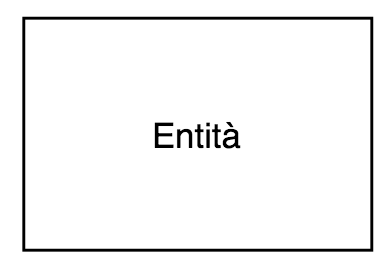
\includegraphics[scale = 0.4]{13/img0}  \\ \hline
        Relazione & 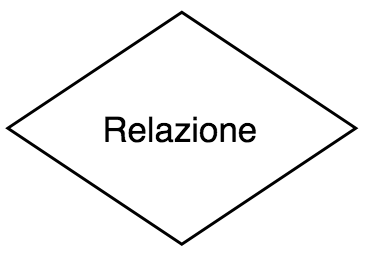
\includegraphics[scale = 0.4]{13/img1}  \\ \hline
        Attributo semplice & 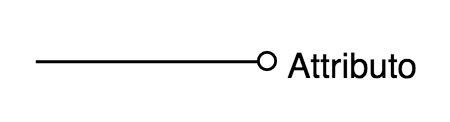
\includegraphics[scale = 0.4]{13/img2}  \\ \hline
        Attributo composto & 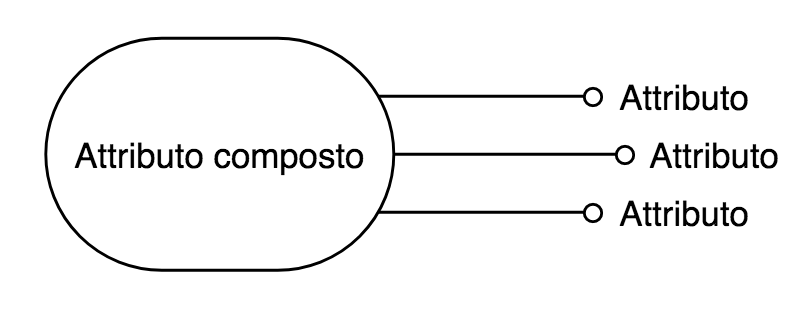
\includegraphics[scale = 0.4]{13/img3}  \\ \hline
        Cardinalità di relazione & 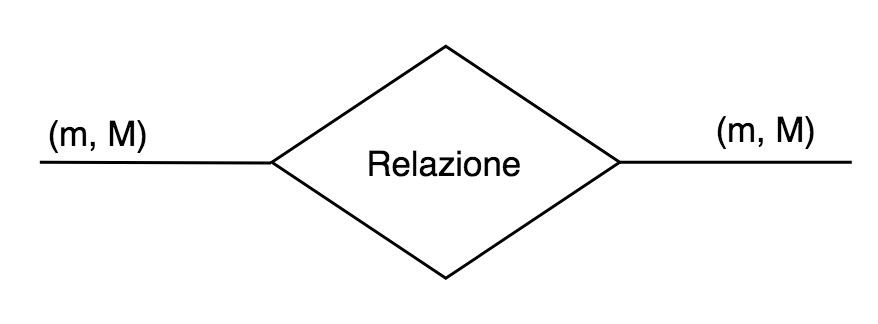
\includegraphics[scale = 0.4]{13/img4}  \\ \hline
        Cardinalità di attributo & 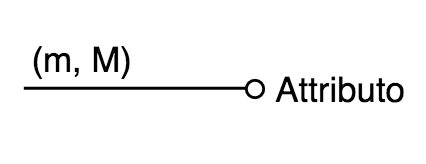
\includegraphics[scale = 0.4]{13/img5}  \\ \hline
        Identificatore interno & 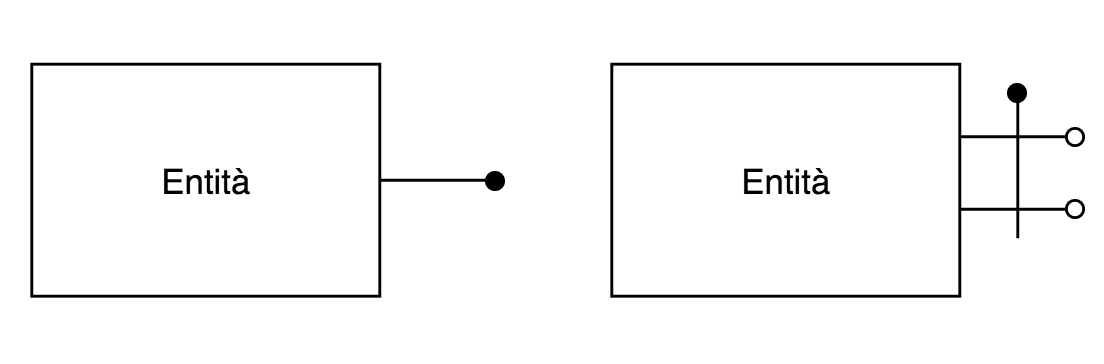
\includegraphics[scale = 0.4]{13/img6}  \\ \hline
        Identificatore esterno & 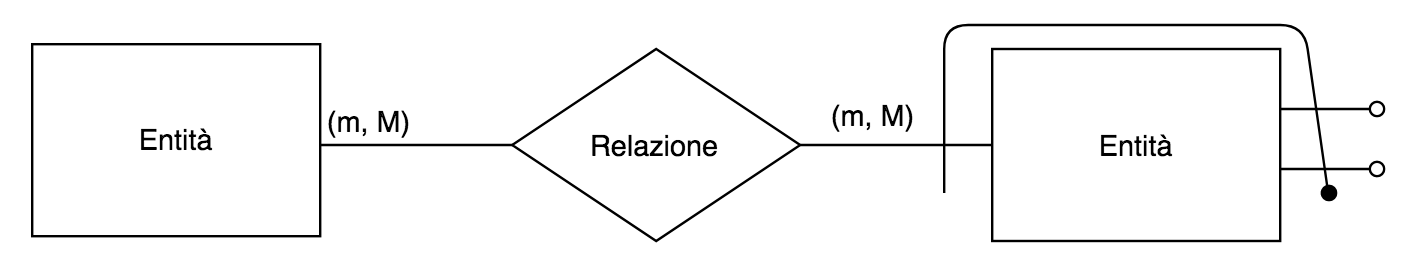
\includegraphics[scale = 0.4]{13/img7}  \\ \hline
        Generalizzazione & 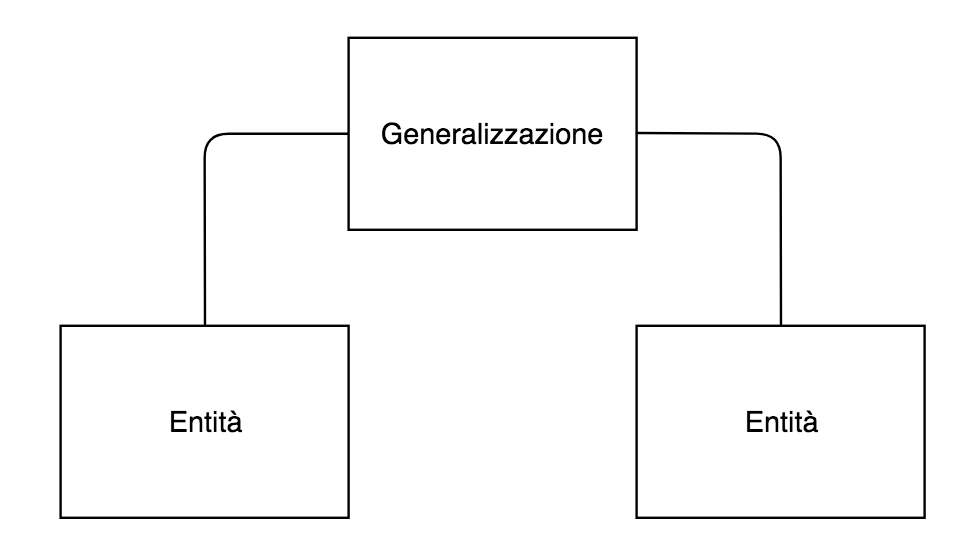
\includegraphics[scale = 0.4]{13/img8}  \\ \hline
        \end{tabular}\end{center}
    \end{table}

\subsection{I costrutti principali del modello}
\textbf{Entità.} Rappresentano classi di oggetti (es. fatti, cose, persone) che hanno proprietà comuni ed esistenza "autonoma" ai fini dell'applicazione d'interesse.\\
Si osservi che un'occorrenza di entità non è un valore che identifica un oggetto, ma è l'oggetto stesso.\\
Un'interessante conseguenza di questo fatto è che un'occorrenza di entità ha un'esistenza (e un'identità) indipendente dalle proprietà ad esso associate.\\
In questo il modello E-R presenta una marcata differenza rispetto al modello relazionale nel quale non possiamo rappresentare un oggetto senza conoscre alcune sue proprietà.\\
In uno schema, ogni entità ha un nome che la identifica univocamente e viene rappresentata graficamente mediante un rettangono con il nome dell'entità all'interno.\\\\
\textbf{Relazioni.} Rappresentano legami logici, significativi per l'applicazione d'interesse tra due o più entità.\\
Un'occorrenza di relazione è un'ennupla (coppia nel caso di relazione binaria) costituita da occorrenze di entità, una per ciascuna delle entità coinvolte.\\
In uno schema E-R, ogni relazione ha un nome che la identifica univocamente e viene rappresentata graficamente mediante un rombo, con il nome della relazione all'interno, e da linee che connettono la relazione con ciascuna delle sue componenti.\\
Possono esistere diverse che coinvolgono le stesse entità (E.G. \texttt{IMPIEGATO} e \texttt{CITTA'} possono essere in relazione \texttt{SEDE} oppure \texttt{RESIDENZA}).\\
Nella scelta dei nomi di relazione è preferibile utilizzare sostantivi invece che verbi, in maniera da non indurre ad assegnare un "verso" alla relazione. (E.g. \texttt{SEDE DI LAVORO} è preferibile a \texttt{LAVORA IN}).\\
L'insieme delle occorrenze di una relazione del modello E-R è, a tutti gli effetti, una relazione matematica tra le occorrenze delle entità coinvolte, ossia, è un sottoinsieme del loro prodotto cartesiano.\\
Questo significa che tra le occorrenze di una relazione del modello E-R non ci possono essere ennuple ripetute.\\
È anche possibile avere relazioni \textbf{ricorsive}, ovver relazioni tra un'entità e se stessa.\\
È infine possibile avere relazioni $n$-arie, relazioni, cioè, che coinvolgono più di due entità.\\\\
\textbf{Attributi.} Descrivono le proprietà elementari di entità o relazioni che sono di interesse ai fini dell'applicazione.\\
Un attributo associa a ciascuna occorrenza di entità (o di relazione) un valore appartenente a un insieme, detto \textbf{dominio}. che contiene i valori ammissibili per l'attributo. I domini non vengono riportati nello schema, ma sono generalmente descritti nella documentazione associata.\\
Può risultare comodo, qualche volta, raggruppare attributi di una medesima entità o relazione che presentano affinità nel loro significato o uso: l'insieme di attributi che si ottiene in questa maniera viene detto \textbf{attributo composto}. Per ridurre la complessità degli schemi, gli attributi commposti verranno usati raramente nel seguito preferendo usare, per quanto possibile, attributi atomici.\\\\
\textbf{Cardinalità delle relazioni.} Vengono specificate per ciascuna partecipazione di entità a una relazione e descrivono il numero minimo e massimo di occorrenze di relazione a cui una occorrenza dell'entità può partecipare. Dicono quindi quante volte, in una relazione tra entità, un'occorrenza di una di queste entità può essere legata a occorrenze delle altre entità coinvolte.\\
\textbf{E.G.:} se in una relazione \texttt{ASSEGNAMENTO} tra due entità \texttt{IMPIEGATO} e \texttt{INCARICO} specifichiamo per la prima entità una cardinalità minima 1 a 1 e una cardinalità massima pari a 5, vogliamo indicare che un impiegato può partecipare a un minimo di 1 occorrenza e a un massimo di 5 occorrenze della relazione \texttt{ASSEGNAMENTO}.\\
In linea di principio è possibile assegnare un qualunque intero non negativo a una cardinalità di una relazione con l'unico vincolo che la cardinalità minima deve essere minore o uguale della cardinalità massima. In realtà, nella maggior parte dei casi, è sufficiente utilizzare solo tre valori: zero, uno e il simbolo $N$ (che indica genericamente un intero maggiore di uno). In particolare:
    \begin{itemize}
        \item{Per la cardinalità minima, zero o uno: nel primo caso si dice che la partecipazione dell'entità relativa è \textbf{opzionale}, nel secondo si dice che la partecipazione è \textbf{obbligatoria}.}
        \item{Per la cardinalità massima, uno o molti ($N$): nel primo caso la partecipazione dell'entità relativa può essere vista come una funzione (parziale se la cardinalità minima vale zero) che associa a un'occorrenza dell'entità una sola occorrenza (o nessuna) dell'altra entità che partecipa alla relazione; nel secondo, invece, c'è un'associazione con un numero arbitrario di occorrenze dell'altra entità.}    
    \end{itemize}
Osservando le cardinalità massime, è possibile classificare le relazioni binarie in base al tipo di corrispondenza che viene stabilita tra le occorrenze delle entità coinvolte:  
    \begin{itemize}
        \item{Le relazioni aventi cardinalità massima pari a uno per entrambe le entità coinvolte definiscono una corrispondenza uno a uno tra le occorrenze di tali entità e vengono quindi denominate \textbf{relazioni uno a uno}.}
        \item{Le relazioni aventi un'entità cardinalità massima pari a uno e l'altra con cardinalità massima pari a $N$ sono denominate \textbf{relazioni uno a molti}.}
        \item{Le relazioni aventi cardinalità massima pari a $N$ per entrambe le entità coinvolte, vengono denominate \textbf{relazioni molti a molti}.}
    \end{itemize}
Per le cardinalità minime, invece, è importante notare che il caso di partecipazione obbligatoria per tutte le entità coinvolte è piuttosto raro, perché quando si aggiunge una nuova occorrenza di entità molto spesso non sono note (o addirittura non esistono) le corrispondenti occorrenze delle entità a esse collegate.\\
Le relazioni non sono necessariamente binarie, possono coinvolgere $n$ attributi, e in tal caso sono dette $n$-arie. Nelle relazioni $n$-arie le entità coinvolte partecipano quasi sempre con cardinalità massima pari a $N$.\\
Nel caso in cui un'entità partecipa a una relazione $n$-aria con cardinalità massima pari a uno, significa che ogni sua occorrenza può essere legata a una sola occorrenza della relazione e quindi a un'unica ennupla di occorrenze delle altre entità coinvolte nella relazione. Questo significa che è possibile (e risulta a volte più naturale) eliminare la relazione $n$-aria e legare direttamente tale entità con altre entità, mediante delle relazioni binarie di tipo uno a molti.\\\\
\textbf{Cardinalità degli attributi.} Possono essere specificate per gli attributi di entità o relazioni e descrivono il numero minimo e massimo di valori dell'attributo associati a ogni occorrenza di entità o relazione. Nella maggior parte dei casi, la cardinalità di un attributo è pari a $(1,1)$ e viene omessa. In questi casi l'attributo rappresenta sostanzialmente una funzione che associa a ogni occorrenza di entità un solo valore dell'attributo.\\
Il valore per un certo attributo può essere però nullo, oppure possono esistere diversi valori di un certo attributo per un'occorrenza di entità. Queste situazioni si possono rappresentare associando all'attributo in questione una cardinalità minima pari a zero nel primo caso e una cardinalità massima pari a $N$, nel secondo.\\
In maniera simile alle partecipazioni delle occorrenze di entità alle relazioni, diremo che un attributo con cardinalità minima pari a zero è \textbf{opzionale} per la relativa entità o relazione, mentre è \textbf{obbligatorio} se la cardinalità minima è pari a uno. Diremo che un attributo è \textbf{multivalore} se la sua cardinalità massima è pari a $N$.\\
In molte situazioni reali accade che certe informazioni non sono disponibili, ed è quindi utile avere la possibilità di specificare attributi opzionali. Gli attributi multivalore vanno invece utilizzati con maggiore cautela, perché essi rappresentano situazioni che possono essere modellate, in alcune occasioni con entità a sé, legate da relazioni uno a molti (o molti a molti) con l'entità cui si riferiscono.\\\\ 
\textbf{Identificatori delle entità.} Vengono specificati per ciascuna entità di uno schema e descrivono i concetti (attributi e/o entità) dello schema che permettono di identificare in maniera univoca le occorrenze delle entità. 
    \begin{itemize}
        \item{In molti casi uno o più attributi di un'entità sono sufficienti a individuare un identificatore: si parla in questo caso di \textbf{identificatore interno} (detto anche \textbf{chiave}).\\
        \textbf{E.G.:} un identificatore interno per l'entità \texttt{AUTOMOBILE} con attributi \texttt{Targa, Colore, Modello} è l'attributo \texttt{Targa}, in quanto non possono esistere due automobili con la stessa \texttt{Targa}.}
        \item{Alcune volte, però, gli attributi di un'entità non sono sufficienti a identificare univocamente le sue occorrenze.\\
        \textbf{E.G.:} Consideriamo l'entità \texttt{STUDENTE}: potrebbe sembrare, a prima vista, che l'attributo \texttt{Matricola} possa essere un identificatore per tale entità, ma ciò non è vero: studenti iscritti a università diverse possono avere lo stesso numero di matricola. Per identificare univocamente uno studente serve, oltre al numero di matricola, anche la relativa università. Quindi, un identificatore corretto per l'entità \texttt{STUDENTE} è costituito dall'attributo \texttt{Matricola} e dell'entità \texttt{UNIVERSITA'}.\\
        Osserviamo che un'entità $E$ può essere identificata da altre entità solo se tali entità sono coinvolte in una relazione a cui $E$ partecipa con cardinalità $(1, 1)$. Nei casi in cui l'identificazione di un'entità è ottenuta utilizzando altre entità si parla di \textbf{identificatore esterno}.\\
        \textbf{E.G.:} Nell'esempio precedente, l'identificazione è resa possibile dalla relazione uno a molti tra le entità \texttt{UNIVERSITA'} e \texttt{STUDENTE}, che associa a ogni studente una e una sola università. Se questa relazione non esistesse, l'identificazione univoca attraverso un'altra entità non sarebbe possibile.}
    \end{itemize}
Sulla base di quanto detto sugli identificatori, è possibile fare alcune considerazioni generali:
    \begin{itemize}
        \item{Un identificatore può coinvolgere uno o più attributi, ognuno dei quali deve avere cardinalità $(1,1)$}
        \item{Un'identificazione esterna può coinvolgere una o più entità, ognuna delle quali deve essere membro di una relazione alla quale l'entità da identificare partecipa con cardinalità $(1,1)$}
        \item{Un'identificazione esterna può coinvolgere un'entità che è a sua volta identificata esternamente, purché non vengano generati, in questa maniera, cicli di identificazioni esterne.}
        \item{Ogni entità deve avere almeno un identificatore (interno o esterno), ma ne può avere in generale più d'uno; nel caso di più identificatori, gli attributi e le entità coinvolte in alcune identificazioni (tranne una) possono essere opzionali (cardinalità minima uguale a zero).}
    \end{itemize}
\textbf{Generalizzazioni.} Rappresentano legami logici tra un'entità $E$, dettà entità \textbf{genitore} e una o più entità $E_1, ..., E_n$ dette entità \textbf{figlie}, di cui $E$ è più generale, nel senso che le comprende come caso particolare. Si dice in questo caso che $E$ è \textbf{generalizzazione} di $E_1, ..., E_n$ e che le entità $E_1, ..., E_n$ sono \textbf{specializzazioni} dell'entità $E$.\\
Tra le entità coinvolte in una generalizzazion valgono le seguenti proprietà generali:
    \begin{itemize}
        \item{Ogni occorrenza di un'entità figlia è anche un'occorrenza dell'entità genitore.}
        \item{Ogni proprietà dell'entità genitore (attributi, identificatori, relazioni e altre generalizzazioni) è anche una proprietà delle entità figlie. Questa proprietà delle generalizzazioni è nota sotto il nome di \textbf{ereditarietà}.}
    \end{itemize}
Le generalizzazioni possono essere classificate sulla base di due proprietà tra loro ortogonali:
    \begin{itemize}
        \item{Una generalizzazione è \textbf{totale} se ogni occorrenza dell'entità genitore è un'occorrenza di almeno una delle entità figlie, altrimenti è \textbf{parziale}.}
        \item{Una generalizzazione è \textbf{esclusiva} se ogni occorrenza dell'entità genitore è al più un'occorrenza di una delle entità figlie, altrimenti è \textbf{sovrapposta}.}
    \end{itemize}

\textbf{Esempi}:
    \begin{itemize}
        \item{Una generalizzazione tra \texttt{PERSONA}, \texttt{UOMO} e \texttt{DONNA} è totale (gli uomini e le donne costituiscono tutte le persone) ed esclusiva (una persona o è uomo o è donna).}
        \item{Una generalizzazione tra l'entittà \texttt{PROFESSIONISTA}, \texttt{INGEGNERE} e \texttt{DOTTORE} è invece parziale (esistono altre professioni altre a queste due) ed esclusiva (assumiamo che ogni professionista abbia una sola professione principale).}
        \item{\textbf{E.G. 3:} Una generalizzazione tra l'entittà \texttt{PERSONA}, \texttt{STUDENTE} e \texttt{LAVORATORE} è una generalizzazione parziale (esistono persone che non sono né studenti né lavoratori) e sovrapposta (esistono studenti che sono anche lavoratori).}
    \end{itemize}
In realtà le generalizzazioni sovrapposte possono essere facilmente trasformate in generalizzazioni esclusive aggiungendo una o più entità figlie, per rappresentare i concetti che costituiscono le intersezioni delle entità che si sovrappongono.\\
\textbf{E.G.}: nel caso degli studenti e dei lavoratori è sufficiente aggiungere l'entità \texttt{STUDENTELAVORATORE} per ottenere una generalizzazione esclusiva.\\
Quindi, nel seguito assumeremo che le generalizzazioni siano sempre esclusive, in quanto questa scelta rende più semplice la traduzione verso il modello relazionale.



\section{Panoramica finale sul modello E-R}
Abbiamo detto più volte che gli schemi E-R costituiscono utili strumenti nell'attività di progettazione di basi di dati. In realtà, tali schemi fornendo rappresentazioni astratte dei dati di un'applicazione, possono essere utilizzati con profitto anche per attività non strettamente legate alla progettazione.\\\\
Si possono fare i seguenti esempi:
    \begin{itemize}
        \item{Gli schemi E-R possono essere utilizzati a scopo documentativo, poiché sono facilmente comprensibili anche da non specialisti di basi di dati.}
        \item{Gli schemi E-R possono essere utilizzati per descrivere i dati di un sistema informativo già esistente (per esempio, per integrarlo con altri) e, nel caso di sistema costituito da diversi sottosistemi, c'è il vantaggio di poter rappresentare le varie componenti con un linguaggio astratto e quindi unificante.}
        \item{Gli schemi E-R possono essere utilizzati per comprendere, in caso di modifica dei requisiti di un'applicazione, su quali porzioni del sistema si deve operare e in cosa consistono le modifiche da effettuare.}
    \end{itemize}



\section{Documentazione di schemi E-R}
Uno schema E-R non è quasi mai sufficiente, da solo, a rappresentare nel dettaglio tutti gli aspetti di un'applicazione, per varie ragioni.
    \begin{itemize}
        \item{Innanzitutto in uno schema E-R compaiono solo i nomi dei vari concetti in esso presenti ma questo può essere insufficiente per comprenderne il significato.}
        {Nel caso di schemi particolarmente complessi, inoltre, può accadere di non riuscire a rappresentare in maniera comprensibile ed esaustiva i vari concetti.}
        \item{Infine, in certi casi addirittura impossibile rappresentare alcune proprietà dei dati attraverso i costrutti che il modello E-R mette a disposizione.\\
        Per esempio, è impossibile rappresentare proprietà che fanno riferimento a due concetti indipendenti (direzione e afferenza) descritti da due relazioni e non esistono costrutti del modello che ci permettono di correlazire due relazioni.\\
        Inoltre, non è possibile esprimere proprietà che corrispondono a vincoli di integrità sui dati.\\
        Infatti, mentre il modello E-R è sufficientemente espressivo per rappresentare dati, risulta meno adatto a rappresentare vincoli complessi su di essi.}
    \end{itemize}
In conclusione, risulta indispensabile corredare ogni schema E-R con una documentazione di supporto, che possa servire a facilitare l'interpretazione dello schema stesso e a descrivere proprietà dei dati rappresentati che non possono essere esprese direttamente dai costrutti del mdoello.\\
Le strutture utilizzate per documentare uno schema E-R non vanno intese come nuovi costrutti di rappresentazione, ma come strumenti, non formali, atti a completare e arricchire la descrizione dei dati di un'applicazione fatta con un modello concettuale.
Vanno quindi considerate come strumenti di supporto all'analisi concettuale ma non possono certamente sostituirsi a essa.

\subsection{Regole aziendali}
Uno degli strumenti più utilizzati per la descrizione di proprietà di un'applicazione che non sono rappresentabili direttamente con i modelli concettuali è quello delle \textbf{regole aziendali} (\textbf{business rules}).\\
Questa terminologia deriva dal fatto che, nella maggior parte dei casi, si vuole esprimere proprio una "regola" del particolare dominio applicativo che stiamo esaminando.\\\\
Possiamo classificare le regole aziendali a seconda della loro natura:
    \begin{itemize}
        \item{\textit{Descrizione di un concetto} rilevante per l'applicazione, ovvero la descrizione precisa di un'entità, di un'attributo o di una relazione del modello ER.}
        \item{\textit{Vincolo di integrità} sui dati dell'applicazione, sia esso la documentazione di un vincolo espresso con qualche costrutto del modello ER, o la descrizione di un vincolo non esprimibile mediante i costrutti del modello.}
        \item{\textit{Derivazione}: un concetto che può essere ottenuto, attraverso un'inferenza o un calcolo aritmetico, da altri concetti dello schema.}
    \end{itemize}
Per le regole del primo tipo si fa in genere ricorso a frasi in linguaggio naturale.\\
Le regole che descrivono vincoli di integrità e derivazioni sono, invece, più adatte a definizioni formali.\\\\
Le regole che descrivono vincoli di integrità possono essere espresse sotto forma di \textbf{asserzioni}, ovvero affermazioni che devono essere sempre verificate nella nostra base dati. Tali affermazioni, per motivi di chiarezza, devono essere atomiche (non possono essere decomposte in frasi che costituiscono esse stesse delle asserzioni).\\
Una struttura predefinita per enunciare regole aziendali sotto forma di asserzioni potrebbe essere la seguente:
    \begin{equation}
        <concetto> \quad \text{deve/non deve} \quad <espressione \text{ } su \text{ } concetti>
    \end{equation}
dove i concetti citati possono corrispondere o a concetti che compaiono nello schema ER a cui si fa riferimento, oppure a concetti derivabili da essi.\\\\
Le regole aziendali che esprimono derivazioni possono essere espresse specificando le operazioni (aritmetiche o di altro genere) che permettono di ottenere il concetto derivato.\\
Una possibile sintassi è la seguente:
    \begin{equation}
        <concetto> \quad \text{si ottiene} \quad <operazione \text{ } su \text{ } concetti>
    \end{equation}
Ovviamente, quando lo schema concettuale viene tradotto in una base di dati (fase di progettazione logica o fisica),  le regole aziendali non descrittive vanno codificate per garantire la consistenza dei dati rispetto alle proprietà che esse rappresentano.

\subsection{Tecniche di documentazione}
Uno schema ER va corredato con una documentazione di supporto, per facilitare l'interpretazione dello schema stesso e per descrivere proprietà dei dati che non possono essere espresse direttamente dai costrutti del modello.\\\\
La documentazione dei vari concetti rappresentati in uno schema, ovvero le regole aziendali di tipo descrittivo, può essere prodotta facendo uso di un \textbf{dizionario dei dati}. Esso è composto da due tabelle: la prima descrive le \textit{entità} dello schema con il nome, una definizione informale in linguaggio naturale, l'elenco di tutti gli attributi (con eventuali descrizioni associate) e i possibili identificatori.\\
L'altra tabella descrive le \textit{relazioni} con il nome, una loro descrizione informale, l'elenco degli attributi (con eventuali descrizioni) e l'elenco delle entità coinvolte insieme alla loro cardinalità di partecipazione.\\\\
L'uso del dizionario è particolarmente importante nei casi in cui lo schema è complesso, (molti concetti collegati in maniera articolata) e risulta pesante specificare direttamente sullo schema tutti gli attributi di entità e relazioni.\\\\
Per quel che riguarda le altre regole aziendali, si può far ricorso ancora a una tabella, nella quale vengono elencate le varie regole, specificando di volta in volta la loro tipologia.
\chapter{Progettazione Concettuale}



\section{Raccolta e analisi dei requisiti}
Per \textbf{raccolta dei requisiti} si intende la completa individuazione dei problemi che l'applicazione da realizzare deve risolvere e le caratteristiche che tale applicazione dovrà avere.\\ 
Per caratteristiche del sistema si intendono sia gli aspetti statici (i dati) che gli aspetti dinamici (le operazioni sui dati).\\
Dato che i requisiti vengono inizialmente raccolti in specifiche espresse generalmente in linguaggio naturale, risultano spesso ambigui e disorganizzati.\\\\
L'\textbf{analisi dei requisiti} consiste nel chiarimento e nell'organizzazione delle specifiche dei requisiti.

\subsection{Fonti dei requisiti}
Per la raccolta dei requisiti possiamo rivolgerci a diverse fonti, che rientrano solitamente in una delle seguenti categorie:
    \begin{itemize}
        \item{\textbf{Utenti dell'applicazione}: le operazioni si acquisiscono mediante opportune interviste, oppure attraverso una documentazione scritta che gli utenti possono avere predisposto appositamente.}
        \item{\textbf{Documentazione esistente}: documentazione che ha qualche attinenza con il problema che stiamo studiando (moduli, regolamenti interni, procedure aziendali, normative). \\
        È richiesta, in questo caso, un'attività di raccolta e selezione che viene assistita dagli utenti, ma è sempre a carico del progettista.}
        \item{\textbf{Realizzazioni pre-esistenti}: applicazioni che devono essere rimpiazzate oppure che devono interagire in qualche maniera con il sistema da realizzare.\\
        La conoscenza delle caratteristiche di queste applicazioni potrebbe fornirci importanti informazioni anche in relazione ai problemi esistenti che è necessario risolvere.}
    \end{itemize}

\subsection{Specifica dei requisiti}
La specifica dei requisiti raccolti avviene spesso facendo uso di descrizioni in linguaggio naturale. Sappiamo, però, che il linguaggio naturale è fonte di ambiguità e fraintendimenti.\\
È molto importante, quindi, effettuare una profonda analisi del testo che descrive le specifiche per filtrare le eventuali inesattezze e i termini ambigui presenti.\\\\
Ecco alcune regole generali per ottenere una specifica dei requisiti più precisa e senza ambiguità:
    \begin{enumerate}
        \item{\textbf{Scegliere il corretto livello di astrazione}: è bene evitare di utilizzare termini \textit{troppo generici} o \textit{troppo specifici}, che rendono poco chiaro un concetto.}
        \item{\textbf{Standardizzare la struttura delle frasi}: nella specifica dei requisiti preferibile utilizzare sempre lo stesso stile sintattico.\\
        Per esempio:
            \begin{equation}
                \text{Per} \quad <dato> \qquad
                \text{rappresentiamo} \quad <insieme \text{ } di \text{ } proprieta>
            \end{equation}}
        \item{\textbf{Evitare frasi contorte}: le definizioni devono essere semplici e chiare.}
        \item{\textbf{Individuare sinonimi/omonimi e unificare i termini}: i sinonimi indicano termini diversi con lo stesso significato; gli omonimi indicano termini uguali con diversi significati.\\
        Queste situazioni possono generare ambiguità e vanno chiarite: nel caso di sinonimi unificando i termini, nel caso di omonimi utilizzando termini diversi o specificandoli meglio.}
        \item{\textbf{Rendere esplicito il riferimento tra termini}: può succedere che l'assenza di di un contesto di riferimento renda alcuni concetti ambigui: in questi casi bisogna esplicitare il riferimento tra termini.}
        \item{\textbf{Costruire un glossario dei termini}: è molto utile per la comprensione e la precisazione dei termini usati, definire un glossario che, per ogni termine, contenga: una breve descrizione, possibili sinonimi e altri termini contenuti nel glossario con i quali esiste un legame logico.}
    \end{enumerate}

    \begin{table}[h!]
        \begin{tabularx}{\textwidth}{|c|X|c|c|} \hline
            \textbf{Termine} & \textbf{Descrizione} & \textbf{Sinonimi} & \textbf{Collegamenti} \\ \hline
            ... & ... & ... & ... \\ \hline
        \end{tabularx}
        \caption{Glossario dei termini}
    \end{table}

\subsection{Specifiche sulle operazioni}
Accanto alle specifiche sui dati, vanno raccolte le specifiche sulle operazioni da effettuare su tali dati.
È opportuno cercare di impiegare la stessa terminologia usata per i dati (possiamo fare riferimento al glossario dei termini) e informarci anche sulla frequenza con la quale le varie operazioni vengono eseguite.



\section{Criteri per la rappresentazione dei dati}

\subsection{Criteri generali di rappresentazione}
Pur specificando che non esiste una rappresentazione univoca di un insieme di specifiche, è utile avere delle indicazioni sulle scelte più opportune.
    \begin{enumerate}
        \item{Se un concetto ha proprietà significative e/o descrive classi di oggetti con esistenza autonoma, è opportuno rappresentarlo con una \textbf{entità}.}
        \item{Se un concetto ha una struttura semplice e non possiede proprietà rilevanti associate, è opportuno rappresentarlo con un attributo di un altro concetto a cui si riferisce.}
        \item{Se sono state individuate due (o più) entità e nei requisiti compare un concetto che le associa, questo concetto può essere rappresentato da una relazione.}
        \item{Se uno o più concetti risultano essere casi particolari di un altro, è opportuno rappresentarli facendo uso di una generalizzazione.}
    \end{enumerate}

\subsection{Qualità di uno schema concettuale}
Nella costruzione di uno schema concettuale vanno garantite alcune proprietà generali che uno schema concettuale di buona qualità deve possedere.

\subsubsection{Correttezza}
Uno schema concettuale è \textbf{corretto} quando utilizza propriamente i costrutti messi a disposizione dal modello concettuale di riferimento.\\
Come avviene nei linguaggi di programmazione, gli errori possono essere di due tipi:
    \begin{itemize}
        \item{\textbf{Errori sintattici}: riguardano un uso non ammesso di costrutti.\\
        E.g. una generalizzazione tra relazioni invece che tra entità.}
        \item{{Errori semantici}: riguardano un uso di costrutti che non rispetta la loro definizione.\\
        E.g. l'uso di una relazione per descrivere il fatto che un'entità è una specializzazione di un'altra}
    \end{itemize}
    
\subsubsection{Completezza}
Uno schema concettuale è \textbf{completo} quando rappresenta tutti i dati di interesse e quando tutte le operazioni possono essere eseguite a partire dai concetti descritti nello schema.

\subsubsection{Leggibilità}
Uno schema concettuale è \textbf{leggibile} quando rappresenta i requisiti in maniera naturale e facilmente comprensibile.\\
Per garantire questa proprietà è necessario rendere lo schema autoesplicativo, per esempio, mediante una scelta opportuna dei nomi da dare ai concetti.\\
Inoltre, la leggibilità dipende anche da fattori puramente estetici. Ecco alcuni suggerimenti per rendere lo schema più leggibile:
    \begin{itemize}
        \item{Disporre i costrutti su una griglia scegliendo come elementi centrali quelli con più legami (relazioni) con altri.}
        \item{Tracciare solo linee perpendicolari e cercare di minimizzare le intersezioni.}
        \item{Disporre le entità che sono generalizzazioni sopra le relative entità figlie.}
    \end{itemize}
    
\subsubsection{Minimalità}
Uno schema è \textbf{minimale} quando tutte le specifiche sui dati sono rappresentate una sola volta nello schema. Uno schema, quindi, non è minimale quando esistono delle \textbf{ridondanze}, ovvero concetti che possono essere derivati da altri.\\
A differenza delle altre proprietà, comunque, non sempre una ridondanza è indesiderata, ma può nascere da precise scelte di progettazione.
\chapter{Progettazione Logica}
L'obiettivo della progettazione logica è quello di costruire uno schema logico in grado di descrivere in maniera corretta ed efficiente tutte le informazioni contenute nello schema E-R prodotto nella fase di progettazione concettuale.\\
Non si tratta di una semplice traduzione da un modello a un altro, in quanto, prima di passare allo schema logico, lo schema E-R va ristrutturato per soddisfare due esigenze: quella di semplificare la traduzione e quella di ottimizzare il progetto.\\
La semplificazione dello schema si rende necessaria perché non tutti i costrutti del modello E-R hanno una traduzione naturale nei modelli logici. Per esempio, mentre un'entità può essere facilmente rappresentata da una relazione del modello relazionale (avente gli stessi attributi dell'entità), per le generalizzazioni esistono varie alternative.\\
Inoltre, mentre la progettazione concettuale ha come obbiettivo la rappresentazione accurata e naturale dei dati d'interesse dal punto di vista del significato che hanno nell'applicazione, la progettazione logica costituisce la base per l'effettiva realizzazione dell'applicazione e deve tenere conto, per quanto possibile, delle sue prestazioni: questa necessità può portare a una ristrutturazione dello schema concettuale.



\section{Fasi della progettazione logica}
Le principali fasi della progettazione logica sono le seguenti:
    \begin{itemize}
        \item{\textbf{Ristrutturazione dello schema E-R}: è una fase indipendente dal modello logico scelto e si basa su criteri di ottimizzazione dello schema e di semplificazione della fase successiva.}
        \item{\textbf{Traduzione verso il modello logico}: fa riferimento a uno specifico modello logico (nel nostro caso il modello relazionale) e può includere un'ulteriore ottimizzazione che si basa sulle caratteristiche del modello logico stesso.}
    \end{itemize}
I dati in ingresso della prima fase sono lo schema concettuale prodotto nella fase precedente e il carico applicativo previsto, in termini di dimensione dei dati e caratteristiche delle operazioni.\\
Il risultato che si ottiene è uno schema E-R ristrutturato, che non è più uno schema concettuale nel senso stretto del termine, in quanto costituisce una rappresentazione dei dati che tiene conto degli aspetti realizzativi.\\\\
Questo schema e il modello logico scelto costituiscono i dati in ingresso della seconda fase, che produce lo schema logico della nostra base di dati.\\
In questa seconda fase è possibile effettuare verifiche della qualità dello schema ed eventuali ulteriori ottimizzazioni mediante tecniche basate sulle caratteristiche del modello logico.\\
La tecnica usata nell'ambito del modello relazionale è la \textbf{normalizzazione}.\\
Lo schema logico finale, i vincoli d'integrità definiti su di esso e la relativa documentazione costituiscono i prodotti finali della progettazione logica.



\section{Analisi delle prestazioni su schemi E-R}
Uno schema E-R può essere modificato per ottimizzare alcuni \textbf{indici di prestazione} del progetto. Facciamo riferimento ad indici di prestazione e non di prestazioni perché, in realtà, le prestazioni di una base dati non sono valutabili in maniera precisa in sede di progettazione logica, in quanto dipendenti anche da parametri fisici, dal sistema di gestione di basi di dati che verrà utilizzato e da altri fattori difficilmente prevedibili in questa fase.\\
È comunque possibile, facendo uso di alcune schematizzazioni, effettuare studi di massima dei due parametri che generalmente regolano le prestazioni dei sistemi software:  
    \begin{itemize}
        \item{\textbf{Costo di un'operazione}: viene valutato in termini di numero di occorrenze di entità e associazioni che mediamente vanno visitate per rispondere a un'operazione sulla base di dati.}
        \item{\textbf{Occupazione di memoria}: viene valutato in termini dello spazio di memoria (misurato, per esempio, in numero di byte) necessario per memorizzare i dati descritti dallo schema.}
    \end{itemize}
Per studiare questi parametri, abbiamo bisogno di conoscere (oltre allo schema) le seguenti informazioni:
    \begin{itemize}
        \item{\textbf{Volume dei dati}:
            \begin{itemize}
                \item{Numero di occorrenze di ogni entità e associazione dello schema}
                \item{Dimensioni di ciascun attributo}
            \end{itemize}}
        \item{\textbf{Caratteristiche delle operazioni}:
            \begin{itemize}
                \item{Tipo dell'operazione (interattiva o batch)}
                \item{Frequenza (numero medio di esecuzioni in un certo intervallo di tempo)}
                \item{Dati coinvolti (entità e/o associazioni)}
            \end{itemize}}
    \end{itemize}
Sebbene un'analisi delle prestazioni che fa riferimento a un numero ristretto di operazioni può sembrare riduttiva rispetto al reale carico della base di dati va notato che le operazioni sulle basi di dati seguono la cosiddetta regola \textbf{ottanta-venti}.\\
In base a questa regola, l'ottanta per cento del carico è generato dal venti per cento delle operazioni. Questo fatto ci consente di valutare adeguatamente il carico concetrandoci solo sulle operazioni principali previste.\\\\
Nella \textbf{tavola dei volumi} vengono riportati tutti i concetti dello schema (entità e associazioni) con il volume previsto a regime:
    \begin{table}\caption{Tavola dei volumi}
        \begin{center}\begin{tabular}{|c|c|c|} \hline
        \textbf{Concetto} & \textbf{Tipo} & \textbf{Volume} \\ \hline
        Impiegato & E & 2000 \\ \hline
        Afferenza & R & 1900 \\ \hline
        Dipartimento & E & 80 \\ \hline
        Sede & E & 10\\ \hline
        \end{tabular}\end{center}
    \end{table}
Il volume dei dati e le caratteristiche generali delle operazioni possono essere descritti facendo uso di tabelle, dette \textbf{tavole delle operazioni}, in cui vengono riportati, per ogni operazione, la frequenza prevista e un simbolo che indica se l'operazione è interattiva ($I$) oppure batch ($B$).
    \begin{table}\caption{Tavola delle operazioni}
        \begin{center}\begin{tabular}{|c|c|c|} \hline
        \textbf{Operazioni} & \textbf{Tipo} & \textbf{Frequenza} \\ \hline
        Op.1 & I & 50 al giorno \\ \hline
        Op.2 & I & 100 al giorno \\ \hline
        Op.3 & I & 10 al giorno \\ \hline
        Op.4 & B & 2 a settimana\\ \hline
        \end{tabular}\end{center}
    \end{table}
Nella tavola dei volumi, il numero delle occorrenze delle associazioni dipende da due parametri: il numero di occorrenze delle entità coinvolte nelle associazioni e il numero (medio) di partecipazioni di un'occorrenza di entità alle occorrenze di associazioni.\\
A sua volta, il secondo parametro dipende dalle cardinalità delle associazioni.\\\\ 
Per ogni operazione, possiamo inoltre descrivere graficamente i dati coinvolti con uno \textbf{schema di operazione} che consiste nel frammento dello schema E-R interessato dall'operazione, sul quale viene disegnato il \textit{cammino logico} da percorrere per accedere alle informazioni di interesse.\\
Una volta ottenute queste informazioni, possiamo fare una stima del costo di un'operazione sulla base di dati contando il numero di accessi alle occorrenze di entità e associazioni necessario per eseguire l'operazione.\\\\
Per esprimere le modalità di accesso alle informazioni utilizziamo la \textbf{tavola degli accessi}, che è nella forma:
    \begin{table}\caption{Tavola degli accessi}
        \begin{center}\begin{tabular}{|c|c|c|c|} \hline
        \textbf{Concetto} & \textbf{Costrutto} & \textbf{Accessi} & \textbf{Tipo} \\ \hline
        Impiegato & Entità & 1 & L \\ \hline
        Afferenza & Relazione & 1 & L \\ \hline
        Dipartimento & Entità & 1 & L \\ \hline
        Impiegato & Entità & 1 & L \\ \hline
        \end{tabular}\end{center}
    \end{table}
Nell'ultima colonna di questa tabella viene riportato il tipo di accesso: $L$ per accesso in lettura e $S$ per accesso in scrittura. Questa distinzione va fatta perché, generalmente, le operazioni di scrittura sono più onerose di quelle in lettura (in quanto devono essere eseguite in modo esclusivo e possono richiedere l'aggiornamento di \textbf{indici}, che sono strutture ausiliarie per l'accesso efficiente ai dati).



\section{Ristrutturazione di schemi E-R}
La fase di ristrutturazione di uno shcema E-R si può suddividere in una serie di passi da effettuare in sequenza:
    \begin{itemize}
        \item{\textbf{Analisi delle ridondanze}: si decide se eliminare o mantenere eventuali ridondanze presenti nello schema.}
        \item{\textbf{Eliminazione delle generalizzazioni}: tutte le generalizzazioni presenti nello schema vengono analizzate e sostituite da altri costrutti.}
        \item{\textbf{Partizionamento/accorpamento di entità e associazioni}: si decide se è opportuno partizionare concetti dello schema (entità e/o associazioni) in più concetti o, viceversa, accorpare concetti separati da un unico concetto.}
        \item{\textbf{Scelta degli identificatori principali}: si seleziona un identificatore per quelle entità che ne hanno più di uno.}
    \end{itemize}
    
\subsection{Analisi delle ridondanze}
Ricordiamo che una \textbf{ridondanza} in uno schema concettuale corrisponde alla presenza di un dato che può essere derivato (cioè ottenuto attraverso una serie di operazioni) da altri dati. In particolare, in uno schema E-R si possono presentare diversi tipi di ridondanza:
    \begin{itemize}
        \item{Attributi derivabili, occorrenza per occorrenza, da altri attributi della stessa entità (o associazione).}
        \item{Attributi derivabili da attributi di altre entità (o associazioni) di solito attraverso funzioni aggregative.}
        \item{Attributi derivabili da operazioni di conteggio di occorrenze. Si tratta, in effetti, di una variante del caso precedente, che viene però discusso separatamente perché molto frequente in pratica.}
        \item{Associazioni derivabili dalla composizione di altre associazioni in presenza di cicli. Notiamo che non sempre la presenza di un ciclo genera ridondanze!}
    \end{itemize}
La presenza di un dato derivato presenta un vantaggio e alcuni svantaggi. Il vantaggio è una riduzione degli accessi necessari per calcolare il dato derivato, gli svantaggi sono una maggiore occupazione di memoria (che è, comunque, spesso un costo trascurabile) e la necessità di effettuare operazioni aggiuntive per mantenere il dato derivato aggiornato.\\
La decisione di mantenere o eliminare una ridondanza va quindi presa confrontando costo di esecuzione delle operazioni che coinvolgono il dato ridondante e relativa occupazione di memoria, nei casi di presenza e assenza della ridondanza.

\subsection{Eliminazione delle generalizzazioni}
Dato che i sistemi tradizionali per la gestione delle basi di dati non consentono di rappresentare direttamente una generalizzazione, risulta spesso necessario trasformare questo costrutto in altri costrutti del modello E-R per i quali esiste invece una implementazione naturale: le entità e le associazioni.
     \begin{figure}
        \centering
        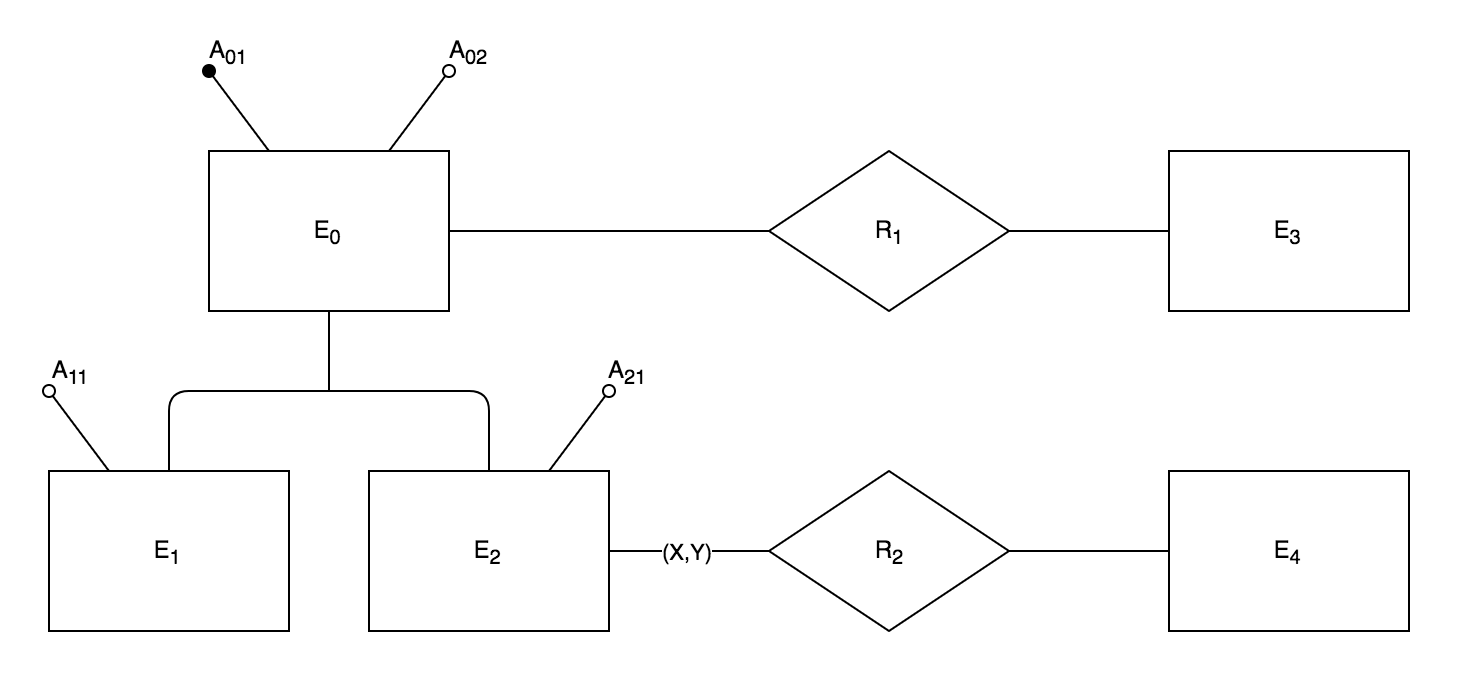
\includegraphics[scale=0.6]{15/img0}
        \caption{Generalizzazione: esempio}
    \end{figure}\\\\
Per rappresentare una generalizzazione mediante entità e associazioni abbiamo essenzialmente tre alternative possibili, che si eseguono attraverso le seguenti ristrutturazioni:
    \begin{enumerate}
        \item{\textbf{Accorpamento delle figlie della generalizzazione nel genitore.}\\
        Le entità $E_1$ ed $E_2$ vengono eliminate e le loro proprietà (attributi e partecipazioni ad associazioni e generalizzazioni) vengono aggiunte all'entità genitore $E_0$.\\
        A tale entità viene aggiunto un ulteriore attributo che serve a descrivere il "tipo" di una occorrenza di $E_0$, cioè se tale occorrenza apparteneva a $E_1$ oppure a $E_2$ o, nel caso di generalizzazione non totale, a nessuna di esse.
            \begin{figure}[h!]
                \centering
                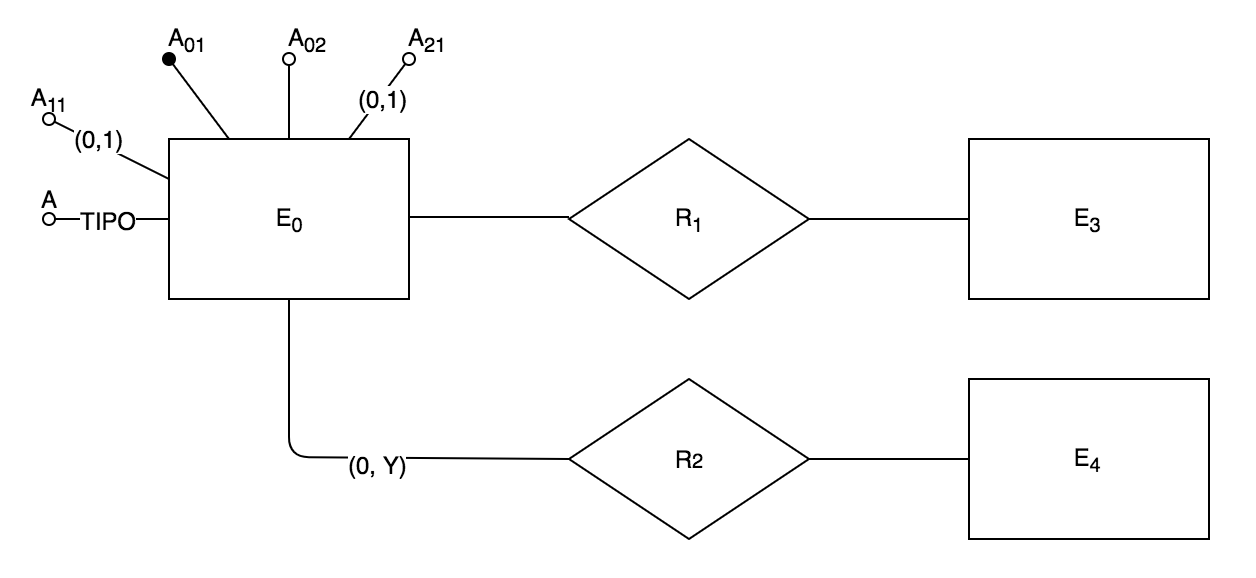
\includegraphics[scale=0.6]{15/img1}
                \caption{Ristrutturazione n.1}
            \end{figure}\\\\}
        \item{\textbf{Accorpamento del genitore della generalizzazione nelle figlie.}\\
        L'entità genitore $E_0$ viene eliminata e, per la proprietà dell'ereditarietà i suoi attributi, il suo identificatore e le relazioni a cui tale entità partecipava, vengono aggiunti alle entità figlie $E_1$ ed $E_2$.\\
        Le relazioni $R_{11}$ e $R_{12}$ rappresentano rispettivamente la restrizione della relazione $R_1$ sulle occorrenze delle entità $E_1$ ed $E_2$.
            \begin{figure}[h!]
                \centering
                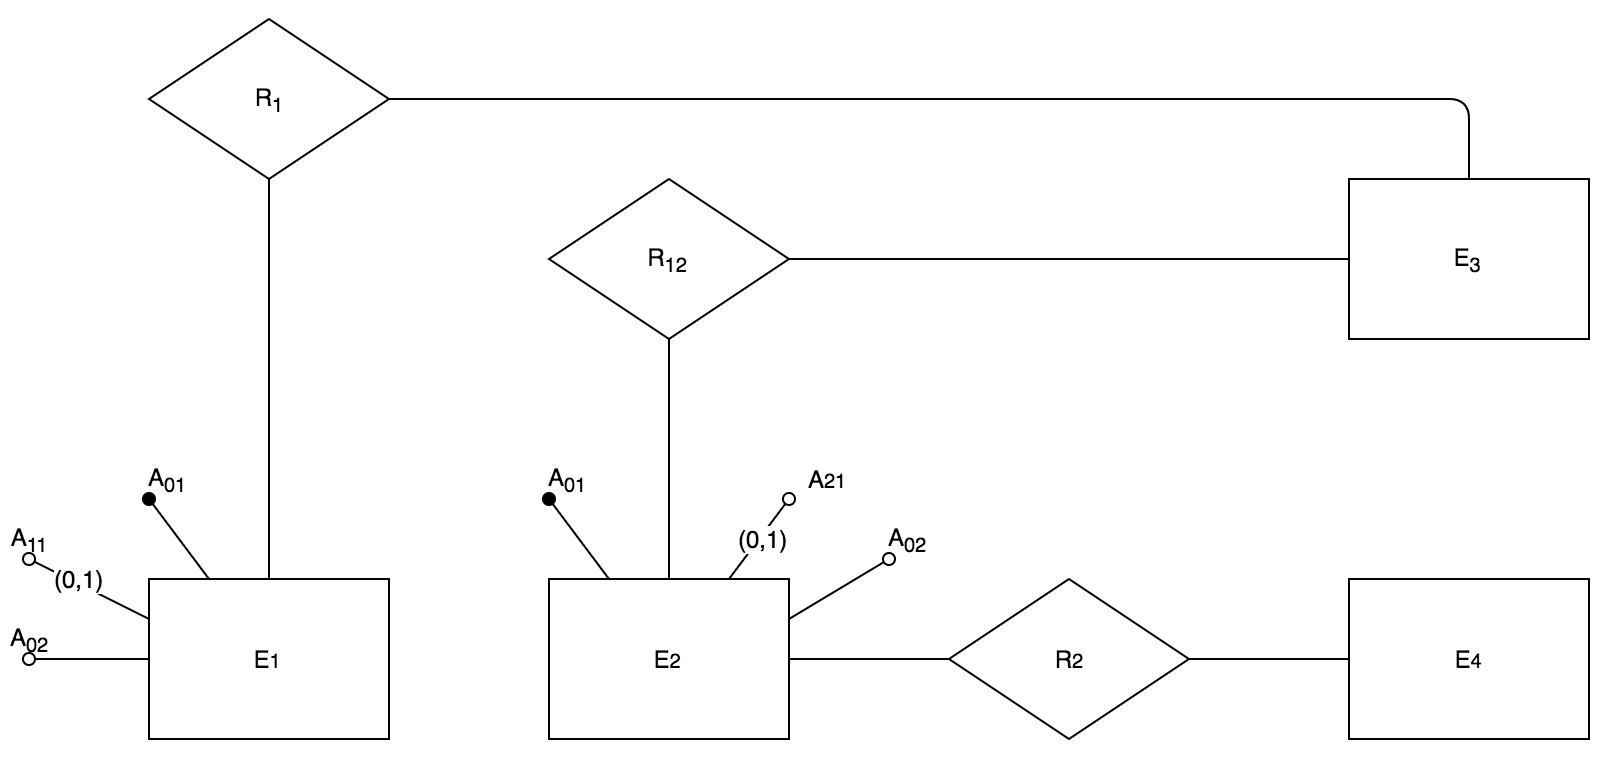
\includegraphics[scale=0.5]{15/img2}
                \caption{Ristrutturazione n.2}
            \end{figure}\\\\}
        \item{\textbf{Sostituzione della generalizzazione con associazioni.}\\
        La generalizzazione si trasforma in due associazioni uno a uno, che legano rispettivamente l'entità genitore con le entità figlie $E_1$ ed $E_2$. Non ci sono trasferimenti di attributi o associazioni e le entità $E_1$ ed $E_2$ sono identificate esternamente dall'entità $E_0$.\\
        Nello schema ottenuto vanno aggiunti, però, dei vincoli: ogni occorrenza di $E_0$ non può partecipare contemporaneamente a $R_{G1}$ e $R_{G2}$; inoltre, se la generalizzazione è totale, ogni occorrenza di $E_0$ deve partecipare o a un'occorrenza di $R_{G1}$ oppure a un'occorrenza di $R_{G2}$.
            \begin{figure}[h!]
                \centering
                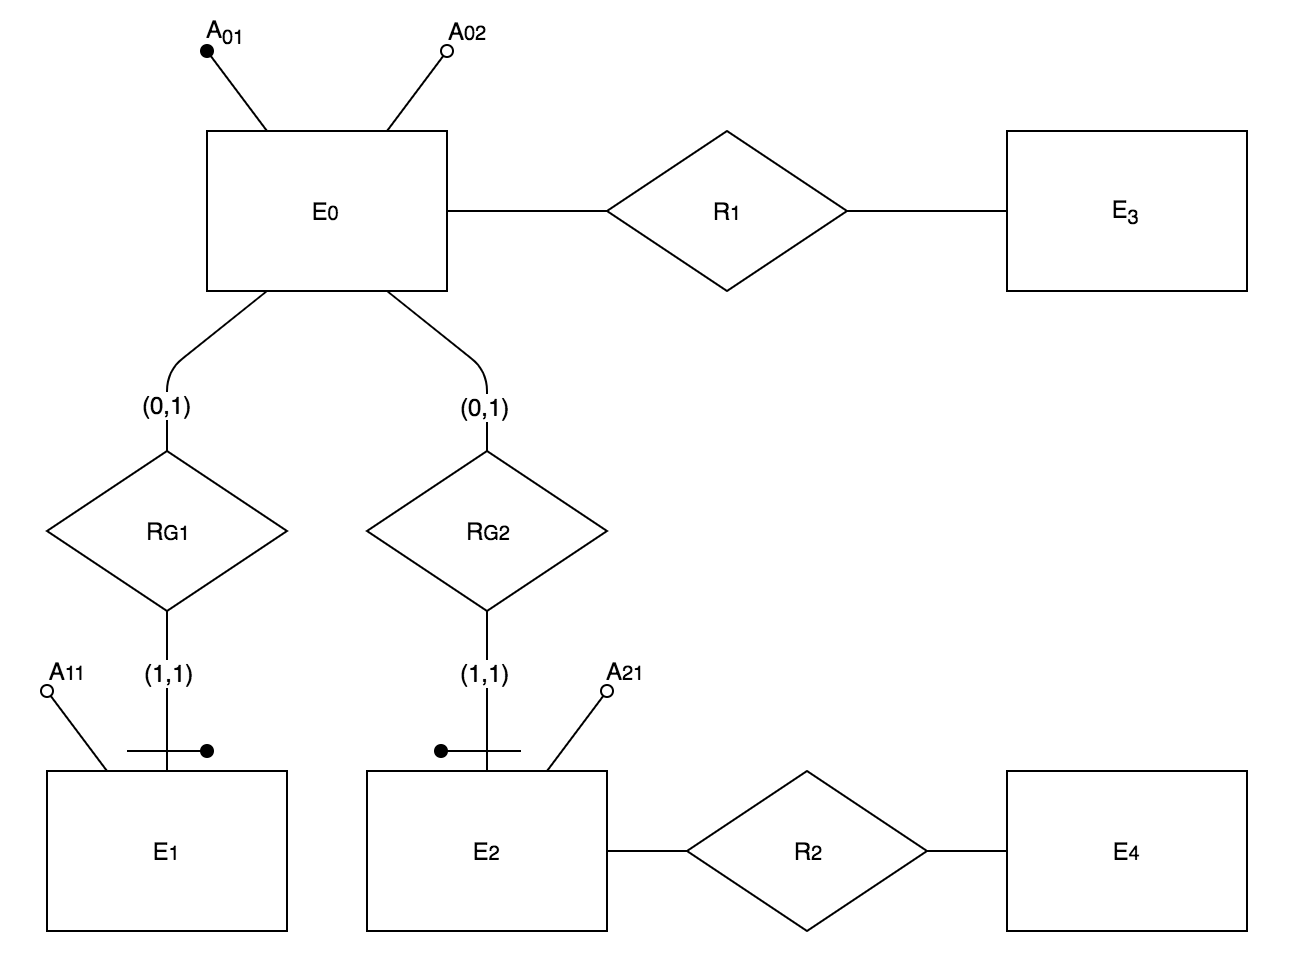
\includegraphics[scale=0.6]{15/img3}
                \caption{Ristrutturazione n.3}
            \end{figure}\\\\}
    \end{enumerate}
La scelta fra le varie alternative può essere fatta in maniera analoga a quanto fatto per i dati derivati, considerando vantaggi e svantaggi di ognuna delle scelte possibili relativamente all'occupazione di memoria e al costo delle operazioni coinvolte.\\
È comunque possibile stabilire alcune regole di carattere generale:
    \begin{enumerate}
        \item{\textbf{Alternativa n. 1}: conveniente quando le operazioni non fanno molta distinzione tra le occorrenze e gli attributi di $E_0$, $E_1$ ed $E_2$.\\
        In questo caso, infatti, anche se abbiamo uno spreco di memoria per la presenza di valori nulli, la scelta ci assicura un numero minore di accessi rispetto alle altre, nelle quali le occorrenze e gli attributi sono distribuiti tra le varie entità.}
        \item{\textbf{Alternativa n. 2}: possibile solo se la generalizzazione è totale, altrimenti le occorrenze di $E_0$ che non sono occorrenze né di $E_1$ né di $E_2$ non sarebbero rappresentate.\\
        È conveniente quando non ci sono operazioni che si riferiscono solo ad occorrenze di $E_1$ oppure di $E_2$, e dunque fanno delle distinzioni tra tali entità.\\
        In questo caso abbiamo un risparmio di memoria rispetto all'alternativa n.1 perché, in linea di principio, gli attributi non assumono mai valori nulli. Inoltre, c'è una riduzione degli accessi rispetto all'alternativa n.3 perché non si deve visitare $E_0$ per accedere ad alcuni attributi di $E_1$ ed $E_2$.}
        \item{\textbf{Alternativa n. 3}: conveniente quando la generalizzazione non è totale (sebbene ciò non sia necessario) e ci sono operazioni che si riferiscono solo a occorrenze di $E_1$ ($E_2$) oppure di $E_0$, e dunque fanno delle distinzioni tra entità figlia ed entità genitore.\\
        In questo caso abbiamo un risparmio di memoria rispetto all'alternativa n.1, per l'assenza di valori nulli, ma c'è un incremento degli accessi per mantenere la consistenza delle occorrenze rispetto ai vincoli introdotti.}
    \end{enumerate}
La ristrutturazione delle generalizzazioni è un tipico caso per il quale il semplice conteggio delle istanze e degli accessi non è sempre sufficiente per scegliere la migliore alternativa possibile.\\
Infatti, in base a quanto abbiamo detto, sembra che l'alternativa n.3 non convenga quasi mai perché richiede molti più accessi a occorrenze delle altre per eseguire le operazioni sui dati. Questa ristrutturazione, però, ha il grosso vantaggio di generare entità con pochi attributi. Come vedremo in seguito, questo si traduce a livello pratico, in strutture logiche di piccole dimensioni per le quali un accesso fisico permette di recuperare molti dati (tuple) in una sola volta.\\
In alcuni casi, quindi, va effettuata un'analisi più fine, che tiene conto di altri fattori quali le dimensioni dei domini degli attributi e la quantità di dati che è possibile recuperare con una sola operazione di accesso a memoria secondaria. 
    
\subsection{Partizionamento/accorpamento di concetti}
Entità e associazioni in uno schema E-R possono essere partizionati o accorpati per garantire una maggiore efficienza delle operazioni in base al seguente principio: gli accessi si riducono separando attributi di uno stesso concetto a cui accediamo attraverso operazioni diverse e raggruppando attributi di concetti diversi a cui accediamo attraverso medesime operazioni. Le stesse tecniche discusse per l'analisi delle generalizzazioni possono essere usate per prendere decisioni di questo tipo.\\\\
È importante notare che, in molti casi, i problemi di partizionamento/accorpamento possono essere rinviati alla fase di progettazione fisica.
\subsubsection{Partizionamenti di entità}
Esistono sostanzialmente due tipi di partizionamenti di entità:
    \begin{itemize}
        \item{\textbf{Partizionamenti verticali}: il concetto viene suddiviso operando sui suoi atttributi.\\
        I partizionamenti verticali generano entità con pochi attributi che possono essere tradotte in strutture logiche sulle quali, con un solo accesso, è possibile recuperare molti dati.}
        \item{\textbf{Partizionamenti orizzontali}: la suddivisione avviene sulle occorrenze dell'entità.\\
        Questo tipo di partizionamenti hanno un effetto collaterale: quello di dover duplicare tutte le associazioni a cui l'entità originaria partecipa. Questo fenomeno può avere delle ripercussioni negative sulle prestazioni del sistema.}
    \end{itemize}
Come per le generalizzazioni, anche in questo caso il semplce conteggio delle occorrenze e degli accessi, non è sempre sufficiente per scegliere la migliore alternativa possibile.
\subsubsection{Eliminazione di attributi multivalore}
Questa ristrutturazione si rende necessaria perché, come per le generalizzazioni, il modello relazionale non permette di rappresentare in maniera diretta questo tipo di attributo.\\
Per eliminare un attributo che ha cardinalità $(1,N)$, partizioniamo l'entità che lo contiene in due entità, tra loro legate da una nuova relazione.
    \begin{figure}
        \centering
        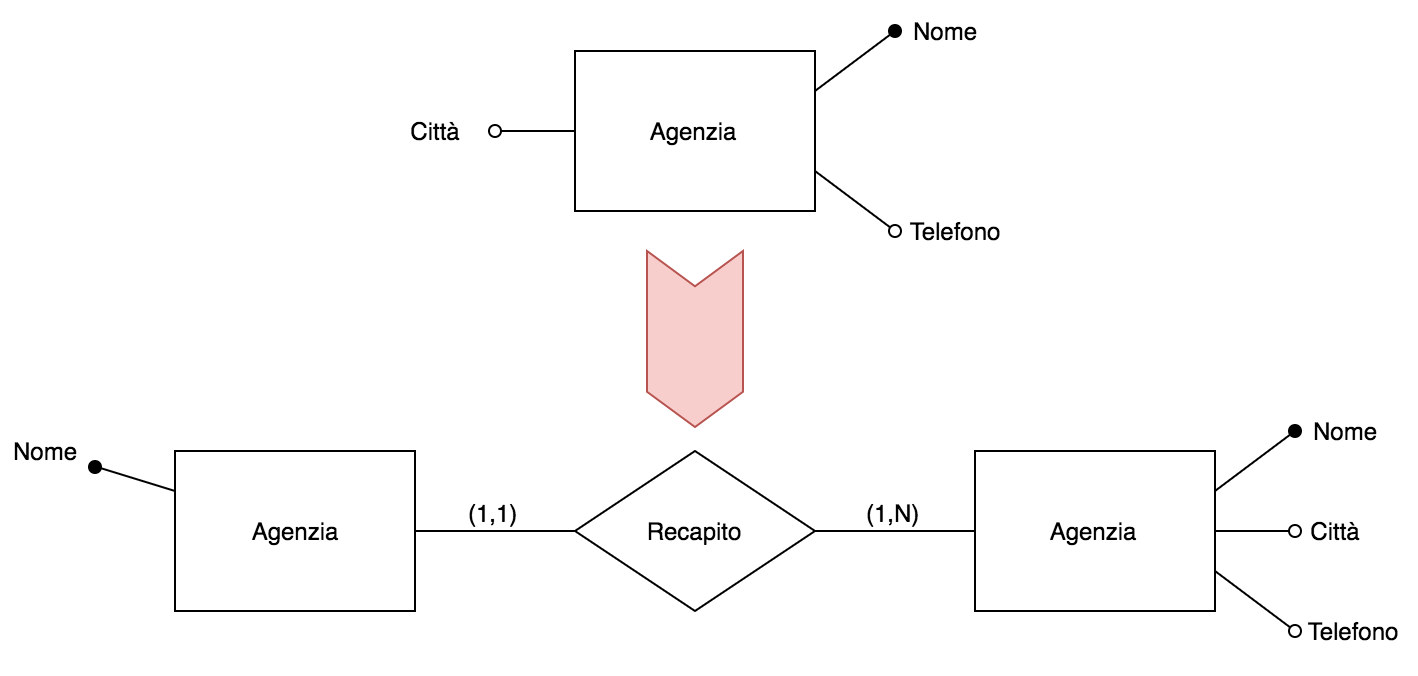
\includegraphics[scale = 0.6]{15/img4}
        \caption{Eliminazione di attributi multivalore}
    \end{figure}\\\\
\subsubsection{Accorpamento di entità}
L'accorpamento è l'operazione inversa del partizionamento.\\
Immaginiamo di avere una relazione $R$ tra due entità $E_1$ ed $E_2$. Nel caso in cui le operazioni sull'entità $E_1$ richiedano sempre i dati relativi ad $E_2$, vogliamo risparmiare gli accessi necessari per risalire a questi dati attraverso $R$. Per farlo, aggiungiamo gli attributi di $E_2$ ad $E_1$, ed eliminiamo $E_2$.\\
Un effetto collaterale di questa ristrutturazione è la possibile presenza di valori nulli causate dalla partecipazione opzionale dell'entità $E_1$ alla relazione $R$.\\
In genere, gli accorpamenti vengono effettuati su associazioni di tipo uno a uno, raramente su relazioni uno a molti e quasi mai su relazioni molti a molti. Questo perché gli accorpamenti di entità legate da un'associazione uno a molti o molti a molti generano ridondanze. In particolare, si possono presentare ridondanze su attributi non chiave dell'entità che partecipava all'associazione originaria con cardinalità massima pari a $N$.\\
La presenza di ridondanze può comunque essere discussa efficacemente attraverso la tecnica della \textbf{normalizzazione}.
\subsubsection{Altri tipi di partizionamento/accorpamento}
I discorsi fatti finora sul partizionamento/accorpamento possono essere estesi alle associazioni. In alcuni casi, infatti, può essere conveniente decomporre un'associazione tra due entità in due (o più) associazioni tra le medesime entità, per separare occorrenze dell'associazione originarie a cui effettuiamo l'accesso sempre separatamente o, viceversa, accorpare due (o più) associazioni tra le medesime entità (che si riferiscono a due aspetti dello stesso concetto) in un'unica associazione, quando accediamo alle relative occorrenze vengono sempre comtemporaneamente.


\subsection{Scelta degli identificatori principali}
La scelta degli identificatori principali è essenziale nelle traduzioni verso il modello relazionale perché in questo modello le chiavi vengono utilizzate per stabilire legami tra dati in relazioni diverse.\\
Inoltre, i sistemi di gestione di basi di dati richiedono generalmente di specificare una \textbf{chiave primaria} sulla quale vengono costruite automaticamente delle strutture ausiliarie, dette \textbf{indici}, per il reperimento efficiente di dati.\\
Quindi, nei casi in cui esistono entità per le quali sono stati specificati più identificatori, bisogna decidere quale di questi identificatori verrà utilizzato come chiave primaria.\\\\
I criteri di decisione per effettuare questa scelta sono i seguenti:
    \begin{itemize}
        \item{Gli attributi con valori nulli non possono costituire identificatori principali. Tali attributi, infatti, non garantiscono l'accesso a tutte le occorrenze dell'entità corrispondente.}
        \item{Un identificatore composto da uno o da pochi attributi è da preferire a identificatori costituiti da molti attributi. Questo garantisce che le strutture ausiliarie create per accedere ai dati (gli indici) siano di dimensioni ridotte, permette un risparmio di memoria nella realizzazione dei legami logici tra le varie relazioni e facilità le operazioni di join.}
        \item{Per le stesse motivazioni esposte al punto precedente, un identificatore interno è da preferire a un identificatore esterno, che magari coinvolge diverse entità.\\
        Infatti, gli identificatori esterni vengono tradotti in chiavi che includono gli identificatori delle entità coinvolte nell'identificazione esterna: chiaramente in questa maniera si possono generare chiavi con molti attributi.}
        \item{Un identificatore che viene utilizzato da molte operazioni per accedere alle occorrenze di un'entità è da preferire rispetto agli altri.\\
        In questa maniera tali operazioni possono essere eseguite efficientemente perché possono trarre vantaggio dagli indici creati automaticamente dal DBMS.}
    \end{itemize}
A questo punto, se nessuno degli identificatori candidati soddisfa tali requisiti, è possibile pensare di introdurre un ulteriore attributo all'entità: questo attributo conterrà valori speciali (detti \textbf{codici}) generati appositamente per identificare le occorrenze delle entità.\\
È comunque consigliabile tenere traccia, in questa fase, anche degli identificatori non selezionati come principali ma che vengono utilizzati da qualche operazione per accedere ai dati. Infatti, per questi identificatori è possibile definire, in sede di progettazione fisica, degli \textbf{indici secondari}. Gli indici secondari consentono l'accesso efficiente ai dati e possono essere usati in alternativa agli indici definiti automaticamente sugli identificatori principali. 

\section{Traduzione verso il modello relazionale}
La seconda fase della progettazione logica corrisponde a una traduzione tra modelli di dati diversi: a partire da uno schema E-R ristrutturato si costruisce uno \textbf{schema logico equivalente}, in grado cioè di rappresentare le medesime informazioni.\\
Coerentemente con quanto già detto, facciamo riferimento a una versione semplificata del modello E-R, che non contiene generalizzazioni e attributi multivalore, e nella quale ogni entità ha un solo identificatore. 

\subsection{Entità e associazioni molti a molti}
Consideriamo il seguente schema:
    \begin{figure}[h!]
        \centering
        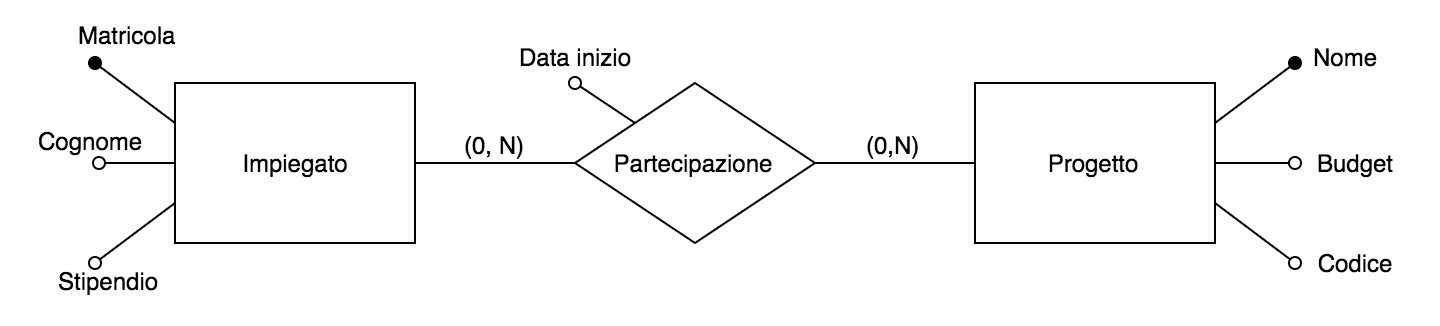
\includegraphics[scale = 0.5]{15/img5}
        \caption{Relazione molti a molti}
    \end{figure}\\\\
La sua traduzione naturale nel modello relazionale prevede:
    \begin{itemize}
        \item{Per ogni entità, una relazione con lo stesso nome avente per attributi i medesimi attributi dell'entità e per chiave il suo identificatore.}
        \item{Per l'associazione, una relazione con lo stesso nome avente per attributi gli attributi dell'associazione e gli identificatori delle entità coinvolte; tali identificatori formano la chiave della relazione.}
    \end{itemize}
Se gli attributi originali di entità o associazioni sono opzionali, i corrispondenti attributi di relazione possono assumere valori nulli.\\
Lo schema relazionale che otteniamo è, quindi, il seguente:
    \begin{equation}\begin{aligned}
        IMPIEGATO(\underline{Matricola}, Cognome, Stipendio)\\
        PROGETTO(\underline{Codice}, Nome, Budget)\\
        PARTECIPAZIONE(\underline{Matricola, Codice}, DataInizio)
    \end{aligned}\end{equation}
Per lo schema ottenuto esistono due vincoli d'integrità referenziale tra gli attributi $Matricola$ e $Codice$ di $PARTECIPAZIONE$ e gli omonimi attributi delle entità $IMPIEGATO$ e $PROGETTO$.\\\\
Possiamo, ovviamente effettuare delle ridenominazioni per rendere lo schema più leggibile, e siamo obbligati a farlo quando abbiamo a che fare con una relazione ricorsiva, come la seguente:
    \begin{figure}[h!]
        \centering
        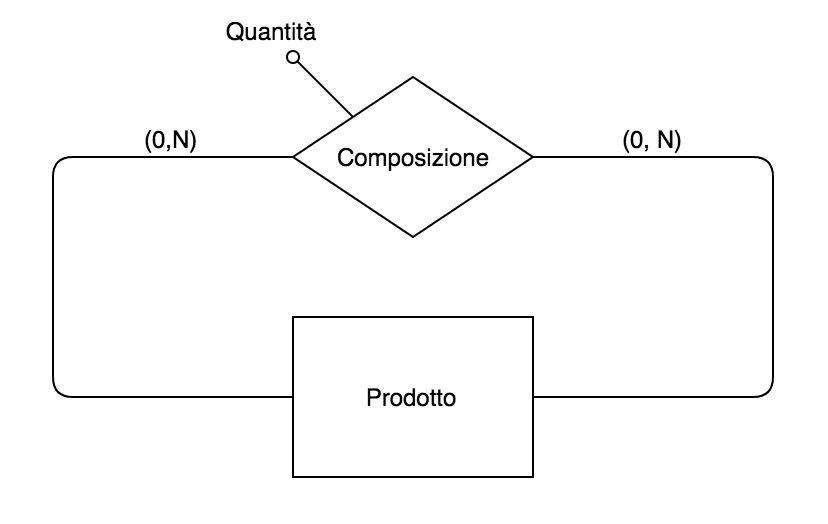
\includegraphics[scale = 0.5]{15/img6}
        \caption{Relazione ricorsiva}
    \end{figure}\\\\
Questo schema si traduce nelle due relazioni
    \begin{equation}\begin{aligned}
        PRODOTTO(\underline{Codice}, Nome, Costo)\\
        COMPOSIZIONE(\underline{Composto, Componente}, Quantita)
    \end{aligned}\end{equation}
In questo schema entrambi gli attributi $Composto$ e $Componente$ contengono codici di prodotti: il primo dei due ha il secondo come componente.\\
Esiste, quindi, un vincolo d'integrità referenziale tra questi attributi e l'attributo $Codice$ della relazione $PRODOTTO$.\\\\
Le associazioni con più di due entità  partecipanti si traducono in maniera analoga a quanto detto per le associazioni binarie.\\
Per esempio, consideriamo il seguente schema:
    \begin{figure}[h!]
        \centering
        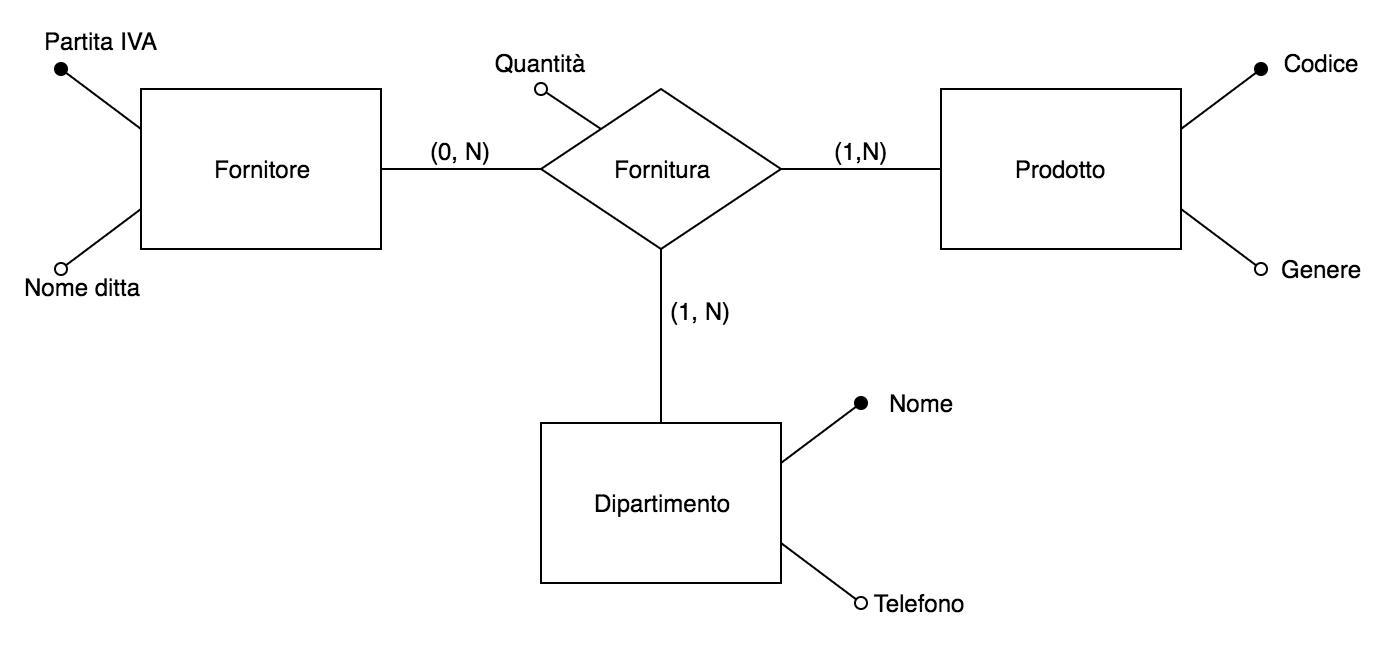
\includegraphics[scale = 0.5]{15/img7}
        \caption{Relazione ternaria}
    \end{figure}\\\\
Questo schema si traduce nelle seguenti relazioni:
    \begin{equation}\begin{aligned}
        FORNITORE(\underline{PartitaIVA}, NomeDitta)\\
        PRODOTTO(\underline{Codice, Genere})\\
        DIPARTIMENTO(\underline{Nome}, Telefono)\\
        FORNITURA(\underline{Fornitore, Prodotto, Dipartimento}, Quantita)
    \end{aligned}\end{equation}
Per lo schema così ottenuto esistono i vincoli d'integrità referenziale tra gli attributi $Fornitore$, $Prodotto$ e $Dipartimento$ della relazione $FORNITURA$ e, rispettivamente, l'attributo $PartitaIVA$ della relazione $FORNITORE$, l'attributo $Codice$ della relazione $PRODOTTO$ e l'attributo $Nome$ della relazione $DIPARTIMENTO$.\\\\
In quest'ultimo tipo di traduzione è necessario prestare attenzione ad alcuni casi particolari nei quali l'insieme delle chiavi delle relazioni che rappresentano le entità coinvolte costituisce in realtà una \textbf{superchiave} ridondante della relazione che rappresenta l'associazione dello schema E-R (esiste cioè un suo sottoinsieme proprio che è una chiave).\\
Questo potrebbe accadere se, per esempio, nel caso della relazione ternaria appena vista, ci fosse un solo fornitore che fornisce un certo prodotto a un dipartimento.\\
Si noti che le cardinalità sono ancora valide, perché tale fornitore può fornire diversi prodotti a questo o altri dipartimenti. In questo caso la chiave della relazione $FORNITURA$ sarebbe costituita dai soli attributi $Prodotto$ e $Dipartimento$, perché dato un prodotto e un dipartimento, il fornitore è univocamente determinato. 

\subsection{Associazioni uno a molti}
Consideriamo il seguente schema:
    \begin{figure}[h!]
        \centering
        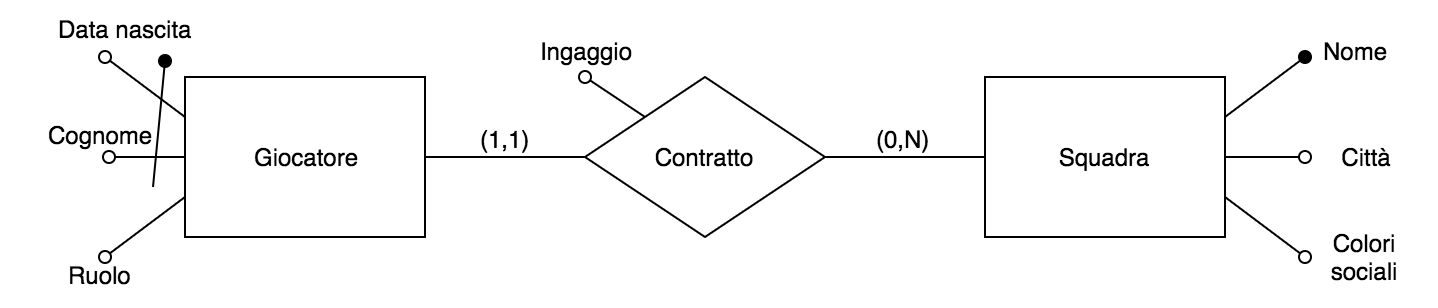
\includegraphics[scale = 0.5]{15/img8}
        \caption{Relazione uno a molti}
    \end{figure}\\\\
Secondo la regola vista per le associazioni molti a molti, la traduzione di questo schema dovrebbe essere la seguente: 
    \begin{equation}\begin{aligned}
        GIOCATORE(\underline{Cognome, DataNascita}, Ruolo)\\
        SQUADRA(\underline{Nome}, Citta, ColoriSociali)\\
        CONTRATTO(\underline{Giocatore, DataNascitaGiocatore}, NomeSquadra, Ingaggio)
    \end{aligned}\end{equation}
Notiamo che nella relazione $CONTRATTO$ la chiave è costituita solo dall'identificatore di $GIOCATORE$ perché le cardinalità indicano che ogni giocatore ha un contratto con una sola squadra.\\
A questo punto le relazioni $GIOCATORE$ e $CONTRATTO$ hanno ancora la stessa chiave ed è ancora possibile fonderle in un'unica relazione (perché esiste una corrispondenza biunivoca tra le rispettive occorrenze). È quindi preferibile la traduzion che segue:
    \begin{equation}\begin{aligned}
        GIOCATORE(\underline{Cognome, DataNascita}, Ruolo, NomeSquadra, Ingaggio)\\
        SQUADRA(\underline{Nome}, Citta, ColoriSociali)
    \end{aligned}\end{equation}
In questo schema, ovviamente, esiste il vincolo d'integrità referenziale tra l'attributo $NomeSquadra$ della relazione $GIOCATORE$ e l'attributo $Nome$ della relazione $SQUADRA$.\\\\
Le associazioni $n$-arie sono quasi sempre molti a molti. Nel caso in cui un'entità partecipi a una relazione ternaria con cardinalità massima pari a uno, la traduzione dell'associazione viene fatta in modo analogo a un'associazione binaria tra le altre entità.\\
L'entità che partecipa alla relazione ternaria con cardinalità massima pari a uno, viene infatti tradotta in una relazione che contiene anche gli identificatori delle altre entità coinvolte nell'associazione (più eventuali attributi dell'associazione stessa) e non è più necessario rappresentare esplicitamente l'associazione di partenza.\\
Consideriamo, per esempio, il seguente schema:
    \begin{figure}[h!]
        \centering
        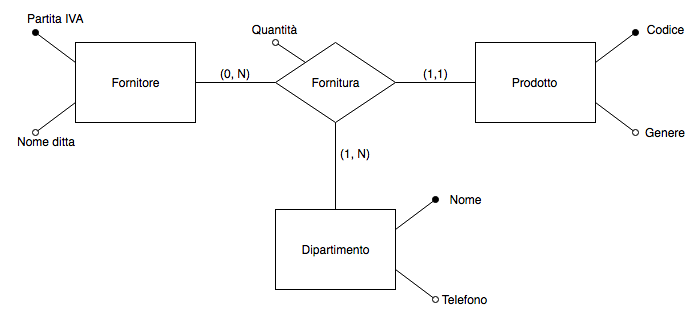
\includegraphics[scale = 0.5]{15/img8b}
        \caption{Relazione uno a molti}
    \end{figure}\\\\
Lo schema si traduce nelle seguenti relazioni:
    \begin{equation}\begin{aligned}
        FORNITORE(\underline{PartitaIVA}, NomeDitta)\\
        DIPARTIMENTO(\underline{Nome}, Telefono)\\
        PRODOTTO(\underline{Codice}, Genere, Fornitore, Dipartimento, Quantita)
    \end{aligned}\end{equation}
In tale schema relazionale esistono i vincoli d'integrità referenziale tra l'attributo $Fornitore$ della relazione $PRODOTTO$ e l'attributo $PartitaIVA$ della relazione $FORNITORE$ e tra l'attributo $Dipartimento$ della relazione $PRODOTTO$ e l'attributo $Nome$ della relazione $DIPARTIMENTO$.    

\subsection{Entità con identificatore esterno}
Le entità con identificatori esterni danno luogo a relazioni con chiavi che includono gli identificatori delle entità "identificanti".\\
Consideriamo il seguente schema:
    \begin{figure}[h!]
        \centering
        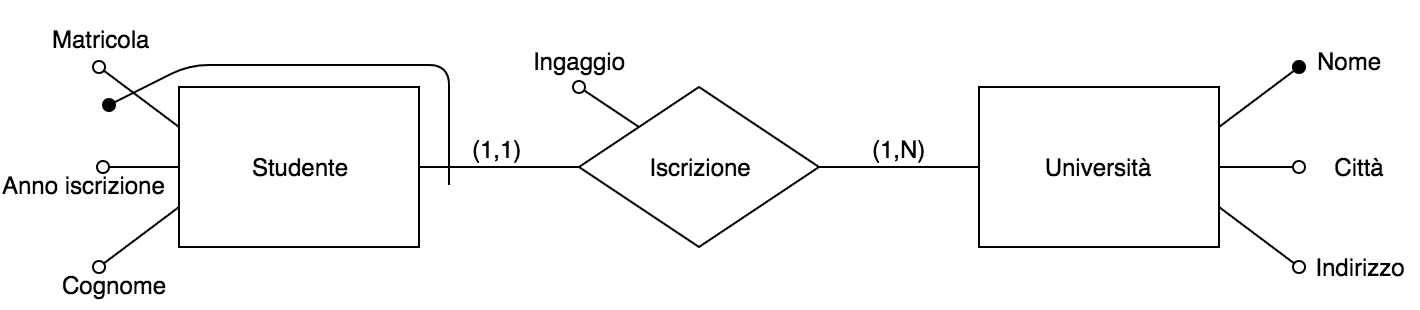
\includegraphics[scale = 0.5]{15/img9}
        \caption{Relazione con identificatore esterno}
    \end{figure}\\\\
Lo schema relazionale corrispondente a questo schema è il seguente:
    \begin{equation}\begin{aligned}
        STUDENTE(\underline{Matricola, NomeUniversita}, Cognome, AnnoIscrizione)\\
        UNIVERSITA(\underline{Nome}, Citta, Indirizzo)
    \end{aligned}\end{equation}
In questo schema relazionale esiste il vincolo d'integrità referenziale tra l'attributo $NomeUniversita$ della relazione $STUDENTE$ e l'attributo $Nome$ della relazione $UNIVERSITA$.\\\\
Come abbiamo potuto notare nell'esempio, rappresentando l'identificatore esterno si rappresenta direttamente anche l'associazione tra le due entità. Le entità identificate esternamente partecipano all'associazione sempre con una cardinalità minima e massima pari a uno.\\
Questo tipo di traduzione è valido indipendentemente dalla cardinalità con cui l'altra entità partecipa all'associazione.

\subsection{Associazioni uno a uno}
Per le associazioni uno a uno ci sono, in genere, diverse possibilità di traduzione.\\
Consideriamo il seguente schema, in cui la partecipazione di entrambe le entità è obbligatoria:
    \begin{figure}[h!]
        \centering
        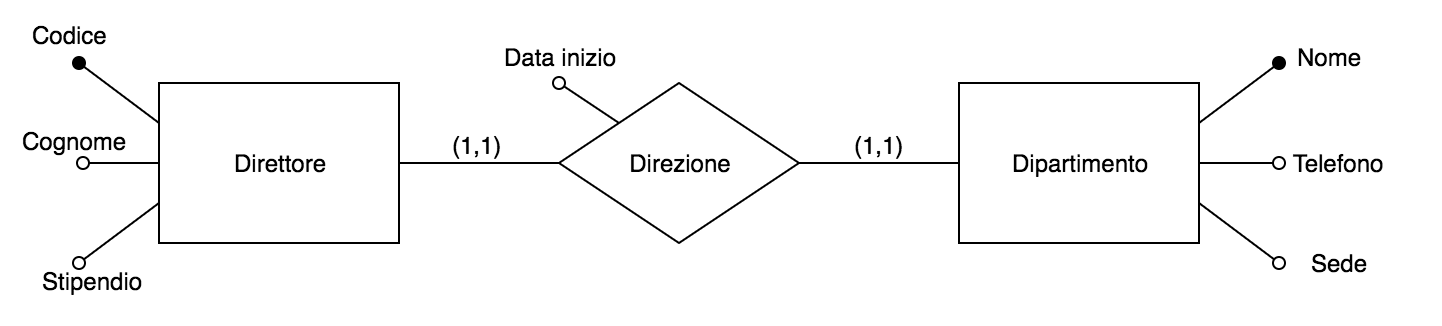
\includegraphics[scale = 0.5]{15/img10}
        \caption{Relazione uno a uno}
    \end{figure}\\\\
Un possibile schema relazionale corrispondente a questo schema è il seguente:
    \begin{equation}\begin{aligned}
        DIRETTORE(\underline{Codice}, Cognome, Stipendio, DipartimentoDiretto, InizioDirezione)\\
        DIPARTIMENTO(\underline{Nome}, Telefono, Sede)
    \end{aligned}\end{equation}
In questo schema esiste il vincolo d'integrità referenziale tra l'attributo $DipartimentoDiretto$ della relazione $DIRETTORE$ e l'attributo $Nome$ della relazione $DIPARTIMENTO$, oppure:
    \begin{equation}\begin{aligned}
        DIRETTORE(\underline{Codice}, Cognome, Stipendio)\\
        DIPARTIMENTO(\underline{Nome}, Telefono, Sede, Direttore, InizioDirezione)
    \end{aligned}\end{equation}
In questo secondo schema esiste il vincolo d'integrità referenziale tra l'attributo $Direttore$ della relazione $DIPARTIMENTO$ e l'attributo $Codice$ della relazione $DIRETTORE$.\\
È possibile, quindi, rappresentare l'associazione in una qualunque delle relazioni che rappresentano le due entità.\\\\
Trattandosi di una relazione biunivoca tra le occorrenze delle entità, sembrerebbe possibile un'ulteriore alternativa nella quale si rappresentano tutti i concetti i un'unica relazione contenente tutti gli attributi in gioco.\\
Questa alternativa è, però, da escludere perché non dobbiamo dimenticare che lo schema E-R che stiamo traducendo è il risultato di una fase di ristrutturazione nella quale sono state effettuate precise scelte anche riguardo l'accorpamento e il partizionamento di entità.\\
Questo significa che, se nello schema E-R ristrutturato abbiamo due entità collegate da una relazione uno a uno, vuol dire che abbiamo ritenuto conveniente tenere separati i due concetti ed è quindi inopportuno fonderli in sede di traduzione verso il modello relazionale.\\\\
Consideriamo ora il seguente schema, in cui soltanto un'unità ha partecipazione opzionale:
    \begin{figure}[h!]
        \centering
        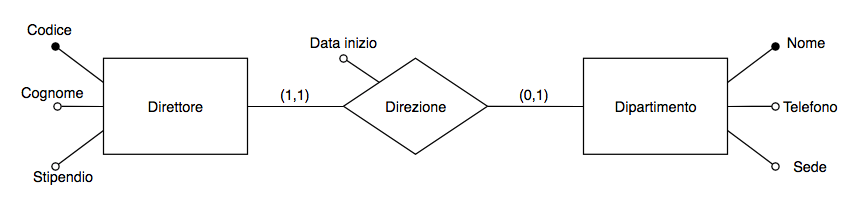
\includegraphics[scale = 0.5]{15/img10b}
        \caption{Relazione uno a uno}
    \end{figure}\\\\
In questo caso abbiamo una soluzione preferibile rispetto alle altre:
    \begin{equation}\begin{aligned}
        IMPIEGATO(\underline{Codice}, Cognome, Stipendio)\\
        DIPARTIMENTO(\underline{Nome}, Telefono, Sede, Direttore, InizioDirezione)
    \end{aligned}\end{equation}
Per lo schema ottenuto esiste il vincolo d'integrità referenziale tra l'attributo $Direttore$ della relazione $DIPARTIMENTO$ e l'attributo $Codice$ della relazione $IMPIEGATO$.\\
Questa alternativa è preferibile rispetto a quella in cui l'associazione viene rappresentata nella relazione $IMPIEGATO$ mediante il nome del dipartimento diretto perché avremmo, per questo attributo, possibili valori nulli.\\\\
Consideriamo ora il caso in cui entrambe le entità hanno partecipazione opizonale, come nel seguente schema:
    \begin{figure}[h!]
        \centering
        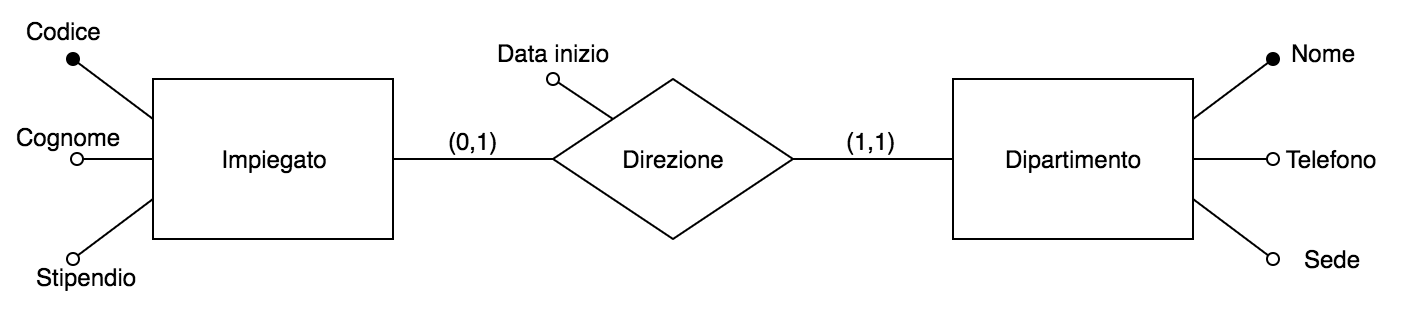
\includegraphics[scale = 0.5]{15/img11}
        \caption{Relazione uno a uno}
    \end{figure}\\\\
In questo caso abbiamo una soluzione preferibile rispetto alle altre:
    \begin{equation}\begin{aligned}
        IMPIEGATO(\underline{Codice}, Cognome, Stipendio)\\
        DIPARTIMENTO(\underline{Nome}, Telefono, Sede)\\
        DIREZIONE(\underline{Direttore}, Dipartimento, DataInizioDirezione)
    \end{aligned}\end{equation}
Su questo schema abbiamo due vincoli d'integrità referenziale: uno tra l'attributo $Direttore$ della relazione $DIREZIONE$ e l'attributo $Codice$ della relazione $IMPIEGATO$ e l'altro tra l'attributo $Dipartimento$ della relazione $DIREZIONE$ e l'attributo $Nome$ della relazione $DIPARTIMENTO$.\\
Questa soluzione ha il vantaggio, rispetto a quella in cui si accorpa la relazione $DIREZIONE$ in una delle altre due relazioni (come nel caso precedente), di non presentare mai valori nulli sugli attributi che rappresentano l'associazione. Per contro, abbiamo bisogno di una relazione in più con un conseguente aumento della complessità della base di dati.\\
Diciamo quindi che la soluzione con tre relazioni è da prendere in considerazione solo se il numero di occorrenze dell'associazione è molto basso rispetto alle occorrenze delle entità che partecipano all'associazione. In questo caso, c'è infatti il vantaggio di evitare la presenza di molti valori nulli.



\section{Documentazione di schemi logici}
Come nel caso della progettazione concettuale, il risultato della progettazione logica non è costituito solo da un semplice schema di una base di dati ma anche da una documentazione a esso associata.\\
Innanzitutto, buona parte della documentazione dello schema concettuale in ingresso alla fase di progettazione logica può essere ereditata dallo schema logico ottenuto come risultato di questa fase. In particolare, se i nomi dei concetti dello schema E-R sono stati riutilizzati per costruire lo schema relazionale, le regole aziendali precedentemente definite possono essere usate per documentare anche quest'ultimo.\\
A questa documentazione ne va aggiunta però dell'altra, in grado di descrivere i vincoli d'integrità referenziale introdotti dalla traduzione.\\\\
A tale riguardo, è possibile adottare un semplice formalismo grafico che ci permette di rappresentare sia le relazioni con i relativi attributi che i vincoli d'integrità referenziale esistenti tra le varie relazioni.\\
Un esempio di tale rappresentazione, di facile comprensione, è dato dal seguente schema:
    \begin{figure}[h!]
        \centering
        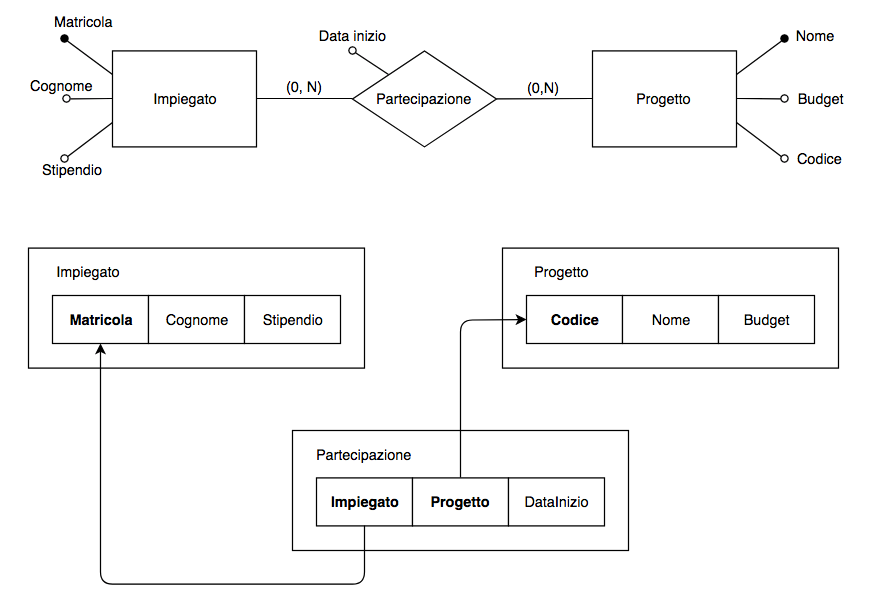
\includegraphics[scale = 0.5]{15/img12}
        \caption{Vincoli d'integrità}
    \end{figure}
In questi diagrammi le chiavi delle relazioni sono rappresentaete in grassetto, le frecce indicano vincoli d'integrità referenziale e la presenza di asterischi sui nomi di attributo indica la possibilità di avere valori nulli.\\\\
Osserviamo che, con questo formalismo, si riesce a mantenere traccia delle associazioni dello schema E-R originale. Questo può risultare utile per individuare, in maniera immediata, i \textbf{cammini di join}, ovvero le operazioni di join necessarie per riscostruire l'informazione rappresentata dalle associazioni originarie, nel caso dell'esempio, le informazioni sui progetti ai quali gli impiegati partecipano, attraverso il join tra $IMPIEGATO$, $PARTECIPAZIONE$ e $PROGETTO$.



\end{document}